\documentclass[12pt]{amsart}

\usepackage{enumerate,amsmath,amssymb,amsthm,mathtools,comment}

\usepackage{arydshln}
\usepackage{dashrule}
\usepackage{slashed}
\usepackage{mathrsfs}
%for Griffiths curly r
\usepackage{calligra}
\DeclareMathAlphabet{\mathcalligra}{T1}{calligra}{m}{n}
\DeclareFontShape{T1}{calligra}{m}{n}{<->s*[2.2]callig15}{}
\newcommand{\scripty}[1]{\ensuremath{\mathcalligra{#1}}}

\newcommand{\capk}{\frac{1}{4 \pi \epsilon_0}}

\begin{document}
\title{}
\author{Alec Hewitt}
\maketitle

\setlength{\parindent}{0mm}

\hdashrule[0.5ex][c]{\linewidth}{0.5pt}{1.5mm}
\begin{center}
These are the derivations that I have been transferring to a Latex document and I plan to add as many as possible  throughout my gap year and review them along the way.
\end{center}
\hdashrule[0.5ex][c]{\linewidth}{0.5pt}{1.5mm}



\section*{QFT}
\section*{\underline{Chapter 2}}

$\mathcal{L}=\frac{1}{2} ( \partial_{\mu} A_{\nu}) (\partial^{\mu}  A^{\nu}) + \frac{1}{2}(\partial_{\mu} A^{\mu})^2;\,\, A^{\mu} \rightarrow (\phi,A^i)$ (Lagrangian for source-less EM field)


\hdashrule[0.5ex][c]{\linewidth}{0.5pt}{1.5mm}

\begin{enumerate}
\setcounter{enumi}{425}

\item \underline{$\partial_{\mu} F^{\mu \nu}=0$; $F^{\mu \nu} = \partial^{\mu} A^{\nu} - \partial^{\nu} A^{\mu}$ (field strength tensor)}\\
\underline{recall:} \{$\mathcal{L}=\frac{1}{2} ( \partial_{\mu} A_{\nu}) (\partial^{\mu}  A^{\nu}) + \frac{1}{2}(\partial_{\mu} A^{\mu})^2;\,\,
\partial_{\mu}(\frac{\partial \mathcal{L}}{\partial(\partial_{\mu} \phi)})-\frac{\partial \mathcal{L}}{\partial \phi}=0 \}\\
\implies \partial_{\mu}(\frac{\partial \mathcal{L}}{\partial(\partial_{\mu} A_{\nu})}) - \frac{\partial \mathcal{L}}{\partial A_{\nu}}=0 \\
\frac{\partial \mathcal{L}}{\partial(\partial_{\mu} A_{\nu})}=\frac{\partial}{\partial(\partial_{\mu} A_{\nu})}(-\frac{1}{2}(\partial_{\sigma} A_{\lambda})(\partial^{\sigma} A^{\lambda}) + \frac{1}{2}(\partial_{\rho} A^{\rho})^2)\\
=-\frac{1}{2}(\partial^{\sigma} A^{\lambda} \frac{\partial(\partial_{\sigma} A_{\lambda})}{\partial(\partial_{\mu} A_{\nu})} + \partial_{\sigma} A_{\lambda} \frac{\partial(\partial^{\sigma} A^{\lambda)}}{\partial(\partial_{\mu} A_{\nu})})+ \frac{1}{2} \frac{\partial(\partial_{\rho} A^{\rho})}{\partial(\partial_{\mu} A_{\nu})}(2 \partial_{\rho} A^{\rho})\\$
\underline{Aside:} $\{ \frac{\partial(\partial^{\sigma}A^{\lambda})}{\partial(\partial_{\mu} A_{\nu})}=\eta^{\sigma \alpha} \eta^{\lambda \beta} \frac{\partial(\partial_{\alpha} A_{\beta})}{\partial(\partial_{\mu} A_{\nu})}=\eta^{\sigma \alpha} \eta^{\lambda \beta} \delta_{\alpha}^{\mu} \delta_{\beta}^{\nu}=\frac{\partial(\partial_{\rho} A^{\rho})}{\partial(\partial_{mu} A_{\nu})}=\eta^{\rho \lambda} \frac{\partial(\partial_{\rho} A_{\lambda})}{\partial(\partial_{mu} A_{\nu})}=\eta^{\rho \lambda} \delta^{\mu}_{\rho} \delta_{\lambda}^{\nu}\} \\
=-\frac{1}{2} ( \partial^{\sigma} A^{\lambda} \delta^{\mu}_{\sigma} \delta_{\lambda}^{\nu} + \partial_{\sigma} A_{\lambda} \eta^{\sigma \alpha} \eta^{\lambda \beta} \delta_{\alpha}^{\mu} \delta_{\beta}^{\nu}) + \eta^{\rho \lambda} \delta_{\rho}^{\mu} \delta_{\lambda}^{\nu} \partial_{\sigma} A^{\nu}\\
=-\frac{1}{2}(\partial^{\mu} A^{\nu} + \partial^\mu A^\nu) + \eta^{\mu \nu} \partial_{\rho} A^{\rho}\\
=-\partial^{\mu} A^{\nu} + \eta^{\mu \nu} \partial_{\rho} A^{\rho} = \frac{\partial \mathcal{L}}{\partial(\partial_{\mu} A_{\nu}}\\
\partial_{\mu}(\frac{\partial \mathcal{L}}{\partial ( \partial_{\mu} A_{\nu)}})=-\partial_{\mu} \partial^{\mu} A^{\nu} + \eta^{\mu \nu} \partial_{\mu} \partial_{\rho} A^{\rho}\\
=-\partial_{\mu} \partial^{\mu} A^{\nu} + \partial^{\nu} \partial_{\mu} A^{\mu}=-\partial_{\mu} ( \partial^{\mu} A^{\nu} -\partial^{\nu} A^{\mu})=-\partial_{\mu} F^{\mu \nu}\\$
where $F^{\mu \nu} = \partial^{\mu} A^{\nu} - \partial^{\nu} A^{\mu};\,\, \frac{\partial \mathcal{L}}{\partial A_v}=0\\
\therefore -\partial_{\mu} F^{\mu \nu}=0$


\hdashrule[0.5ex][c]{\linewidth}{0.5pt}{1.5mm}


\hdashrule[0.5ex][c]{\linewidth}{0.5pt}{1.5mm}


\underline{Useful Notes:} $\epsilon_k^{ij} \partial_j B^k = ( \nabla \times \vec{B})^i,\,\, F^{0i} = \partial^0 A^i - \partial^i A^0\\
= \eta^{0 \mu} \partial_{\mu} A^i - \eta^{i \mu} \partial_{mu} \phi = \partial_0 A^i + \partial_i \phi = - E^i;\,\, \eta^{\mu \nu} = (1,-1,-1,-1) (signature)\\
F^{ij}= \epsilon_k^{ij} B^k$


\hdashrule[0.5ex][c]{\linewidth}{0.5pt}{1.5mm} 


\item \underline{$\frac{\partial \vec{E}}{\partial t} = \nabla \times \vec{B};\,\, \nabla \cdot \vec{E} = 0$}\\
$\partial_{\mu} F^{\mu j} = 0 \implies \partial_0 F^{0j} + \partial_i F^{ij} = -\partial_i E^j + \partial_i \epsilon_k^{ij} B^k\\
=-\partial_0 E^j + ( \nabla \times \vec{B})^j = 0 \implies \frac{\partial \vec{E}}{\partial t} = \nabla \times \vec{B}\\
\partial_{\mu} F^{\mu 0} = \partial_{0} F^{00} + \partial_i F^{i0} = \partial_i F^{i0}= \partial_i E^i = \nabla \cdot \vec{E} = 0\\$


\hdashrule[0.5ex][c]{\linewidth}{0.5pt}{1.5mm}


Under $x \rightarrow \Lambda x,\,\, \phi(x) \rightarrow \phi'(x) = \phi(\Lambda^{-1} x)$ ( active transformation)\\
to see why this makes sense consider a temperature scalar field that has a maximum at $x=a$ after the transformation $x \rightarrow \Lambda x$ the new function has a maximum of $x= \Lambda a$ so that $\psi'(\Lambda a) = \psi(a)\\
\implies \psi'(x) = \psi(a=\Lambda^{-1} x) = \psi(\Lambda^{-1} x)$ so $\psi(x) \rightarrow \psi'(x)= \psi(\Lambda^{-1} x)$


\hdashrule[0.5ex][c]{\linewidth}{0.5pt}{1.5mm}


 \item \underline{$H=\frac{1}{2} p^2 + \frac{1}{2} \omega^2 q^2$}\\
\underline{recall:}  $H_0=T+U=\frac{p^2}{2m} + \frac{1}{2} m \omega^2 x^2\\
\implies \frac{1}{\hbar}(\frac{p^2}{2m} + \frac{1}{2} m \omega^2 x^2)=\frac{H_0}{\hbar}:=H\\
\implies \frac{1}{2 \hbar^2}\frac{1}{\frac{m}{\hbar}} (-i\hbar)^2 \frac{\partial^2}{\partial x^2} + \frac{1}{2} \omega^2 \frac{m}{\hbar} x^2 = H\\
\implies \frac{1}{2 \hbar^2} (-i\hbar)^2 \frac{\partial^2}{\partial (\sqrt{\frac{m}{\hbar}} x)^2} + \frac{1}{2} \omega^2 (\sqrt{\frac{m}{\hbar}} x)^2 =H;\,\, q:=\sqrt{\frac{m}{\hbar}} x\\
\therefore \frac{1}{2}p^2 +\frac{1}{2} \omega^2 q^2 = H; \,\, $ since $ \hbar=1$\\
\underline{Shortened:}\\ Take the Hamiltonian and change variables from $x \rightarrow \sqrt{\frac{m}{\hbar}} x$ and $H \rightarrow \frac{H}{\hbar}$ this is a smart way to get rid of the mass in the hamiltonian.


\hdashrule[0.5ex][c]{\linewidth}{0.5pt}{1.5mm}


\item \underline{$a=\sqrt{\frac{\omega}{2}} q + \frac{i}{\sqrt{2\omega}} p$ (annihilation); $a^{\dagger} = \sqrt{\frac{\omega}{2}} q- \frac{i}{\sqrt{2 \omega}} p$ (creation)}\\
\underline{recall:} $\hat{a}_+ = \frac{1}{\sqrt{2 \hbar m \omega}} (m \omega x - i \hat{p})$ (raising operator)\\
$q=\sqrt{\frac{m}{\hbar}} x \implies \hat{a}_+=\frac{1}{\sqrt{2}} ( \frac{m \omega}{\sqrt{\hbar m \omega}} x - i (-i \hbar) \frac{\sqrt{\frac{m}{\hbar}}}{\sqrt{\hbar m \omega}} \frac{\partial}{\partial x \sqrt{\frac{m}{\hbar}}})\\
=\frac{1}{\sqrt{2}}(\sqrt{\omega} \sqrt{\frac{m}{\hbar}} x - i (- i \hbar) \frac{1}{\sqrt{\hbar m \omega}} \sqrt{\frac{m}{\hbar}} \frac{\partial}{\partial \sqrt{\frac{m}{\hbar}} x})\\
=(\sqrt{\frac{\omega}{2}} q - i (-i \hbar) \frac{1}{\sqrt{2 \hbar \omega}} \frac{\partial}{\partial q}=\sqrt{\omega}{2} q - i \frac{1}{2\omega} p$\\
invert $\implies q=\frac{1}{2 \omega}(a+ a^{\dagger}), p=-i \sqrt{\omega}{2} (a- a^{\dagger})$


\hdashrule[0.5ex][c]{\linewidth}{0.5pt}{1.5mm}


\underline{ $[a,a^{\dagger}]=1$}; to make things simpler $c:=\sqrt{\frac{\omega}{2}};\,\, d:=\frac{1}{\sqrt{2 \omega}}$\\
$(a a^{\dagger} f- a^{\dagger} a f)=(cq+idp)(cq-idp)f-(cq-idp)(cq+idp)f\\
=(cq+idp)(cqf-idpf)-(cq-idp)(cqf+idpf)\\
-c^2q^2f-idcqpf+idcpqf+d^2p^2f-(c^2q^2f+idcqpf-idcpqf+d^2p^2 f)\\
=-2idcqpf+2idcpqf=2idc[p,q]f\\
=2i \frac{1}{2}[p,q] f,\,\,[q,p]=i \implies [p,q]=-i\\
\therefore [a,a^{\dagger}]=-i^2 f=f$\\


\hdashrule[0.5ex][c]{\linewidth}{0.5pt}{1.5mm}


\item \underline{$H=\omega(a^{\dagger}a+\frac{1}{2})$}\\
$H=\frac{1}{2} p^2 + \frac{1}{2} \omega^2 q^2 =\frac{1}{2} ((-i \sqrt{\frac{\omega}{2}})^2 (a-a^{\dagger})^2 + \frac{\omega^2}{\sqrt{2 \omega}^2}(a+a^{\dagger})^2)\\
=\frac{1}{2}(-\frac{\omega}{2}(a^2-a a^{\dagger} - a^{\dagger} a+ {a^{\dagger}}^2) + \frac{\omega}{2}(a^2 + a a^{\dagger} + a^{\dagger} a + {a^{\dagger}}^2))\\
=\frac{\omega}{2}(a a^{\dagger} + a^{\dagger} a);\,\, a^{\dagger} a=[a^{\dagger}, a] + a a^{\dagger}\\
\implies a a^{\dagger} = -[a^{\dagger},a]+ a^{\dagger} a \\
H=\frac{\omega}{2} ( a^{\dagger} a - [a^{\dagger},a] + a^{\dagger} a )= \frac{\omega}{2}(2 a^{\dagger} a + 1)\\
\therefore H= \omega(a^{\dagger} a + \frac{1}{2})$


\hdashrule[0.5ex][c]{\linewidth}{0.5pt}{1.5mm}


\item \underline{$[H,a^{\dagger}]=\omega a^{\dagger};\,\, [H,a]=-\omega a$}\\
$H a^{\dagger} - a^{\dagger} H=\omega(a^{\dagger} a + \frac{1}{2} )a^{\dagger} - \omega a^{\dagger}(a^{\dagger} + \frac{1}{2})\\
=\omega(a^{\dagger} a a^{\dagger} - a^{\dagger} a^{\dagger} a)=\omega(a^{\dagger}(1+ a^{\dagger} a)-a^{\dagger} a^{\dagger} a);\,\, use [a,a^{\dagger}]=1\\
=\omega( a^{\dagger} + a^{\dagger} a^{\dagger} a- a^{\dagger} a^{\dagger} a)=\omega a^{\dagger}$


\hdashrule[0.5ex][c]{\linewidth}{0.5pt}{1.5mm}


\item \underline{$H a^{\dagger}|E\rangle=(E+\omega) a^{\dagger} |E\rangle;\,\, Ha|E\rangle = (E-\omega)a|E \rangle$}\\
\underline{recall:} $H |E \rangle = E |E \rangle$\\
$H a |E \rangle;\,\, H a =[H,a] + aH=- \omega a + a H\\
\implies H a | E \rangle = (-\omega a + aH)|E \rangle = (E- \omega) a |E \rangle$\\


\hdashrule[0.5ex][c]{\linewidth}{0.5pt}{1.5mm}


\item \underline{$a |0 \rangle =0$} (ground state)


\hdashrule[0.5ex][c]{\linewidth}{0.5pt}{1.5mm}

\item \underline{$H|0 \rangle = \frac{\omega}{2} |0 \rangle$}\\
$H|0 \rangle = \omega(a^{\dagger} a + \frac{1}{2})|0 \rangle= \frac{\omega}{2} |0 \rangle$


\hdashrule[0.5ex][c]{\linewidth}{0.5pt}{1.5mm}


\item \underline{$|n \rangle = (a^{\dagger})^n |0 \rangle,\,\, (defn?)\,\, H|n \rangle = (n+\frac{1}{2}) \omega |n \rangle$}
 \\(Note that for excited states: $\langle n | n \rangle \neq 1$)\\
 $\underline{Practice:} H | 0 \rangle := \frac{\omega}{2} |0 \rangle;\,\, H|1 \rangle = H a^{\dagger} |0 \rangle = (\frac{\omega}{2} + \omega)|1 \rangle\\$
 or $H|1 \rangle = \omega ( a^{\dagger} a + \frac{1}{2}) | 1 \rangle = \omega(1 + \frac{1}{2} | 1 \rangle$
 
 
 \hdashrule[0.5ex][c]{\linewidth}{0.5pt}{1.5mm}


 \item \underline{$H | n \rangle=(n+\frac{1}{2}) \omega | n \rangle$ }\\
 \underline{Proof:}\\
 $H | 0 \rangle = \omega (a^{\dagger} a + \frac{1}{2}) |0 \rangle = \omega (0 + \frac{1}{2}) | 0 \rangle= \frac{\omega}{2} | 0 \rangle\\$
 assume $H|n \rangle = (n+ \frac{1}{2}) \omega |n \rangle$ want $H| n+1 \rangle = ((n+1) + \frac{1}{2}) \omega | n+1 \rangle\\
 a^{\dagger} H|n \rangle = (n+\frac{1}{2}) \omega a^{\dagger} |n \rangle = (n + \frac{1}{2}) \omega |n+1 \rangle\\
 a^{\dagger} H = [a^{\dagger},H] + H a^{\dagger} = - \omega a^{\dagger} + H a^{\dagger}\\
 a^{\dagger} H| n \rangle = - \omega a^{\dagger} |n \rangle + H | n+ 1 \rangle = (n+\frac{1}{2}) \omega | n+1 \rangle\\
\therefore H | n+1 \rangle = ((n+1) \frac{1}{2}) \omega | n +1 \rangle $


\hdashrule[0.5ex][c]{\linewidth}{0.5pt}{1.5mm}


\item \underline{$\delta^{(3)} ( \vec{x}_2- \vec{x}_1)= \frac{1}{(2 \pi )^3} \int e^{i \vec{p} \cdot ( \vec{x}_2 - \vec{x}_1)} d^3 p$}\\
 \underline{recall:} $\vec{p}= \hbar \vec{k}= \vec{k}$\\
\underline{recall:} $f(x)=\frac{1}{\sqrt{2\pi}} \int_{-\infty}^{\infty} F(k) e^{ikx} dk ;\,\, F(k) = \frac{1}{\sqrt{2\pi}} \int_{-\infty}^{\infty} f(x) e^{-ikx} dx$\\
$f(x)=\delta(x) = \frac{1}{\sqrt{2 \pi}} \int_{\infty}^{\infty} F(k) e^{ikx} dk; \,\, F(k) = \frac{1}{\sqrt{2\pi}} \int_{-\infty}^{\infty} \delta (x) e^{-ikx} dx = \frac{1}{\sqrt{2\pi}}\\
\implies \delta(x) = \frac{1}{2 \pi} \int_{-\infty}^{\infty} e^{ikx} dk\\
\delta^{(3)} ( \vec{x}_2 - \vec{x}_1):= \delta( x_2-x_1) \delta(y_2-y_1) \delta(z_2-z_1)\\
=\frac{1}{(2\pi)^3} \int_{-\infty}^{\infty} e^{ik_x (x_2-x_1)} d k_x \int_{-\infty}^{\infty} e^{ik_y (y_2-y_1)} dk_y \int_{-\infty}^{\infty} e^{ik_z (z_2- z_1)} dk_z = \frac{1}{(2 \pi)^3} \int e^{i \vec{p} \cdot (\vec{x}_2- \vec{x}_1)} d^3 p$
 

\hdashrule[0.5ex][c]{\linewidth}{0.5pt}{1.5mm}


\underline{ $\nabla \phi = \int \frac{d^3 p}{(2 \pi)^3} \frac{1}{\sqrt{2 \omega_{\vec{p}}}} ( i \vec{p} a_{\vec{p}} e^{i \vec{p} \cdot \vec{x}} - i \vec{p} a_{\vec{p}}^{\dagger} e^{-i \vec{p} \vec{x}})$}\\
$(\nabla \phi)_i = \frac{\partial}{\partial x^i} \phi = \frac{\partial}{\partial x^i} \int \frac{d^3 p}{(2 \pi)^3} \frac{1}{\sqrt{2 \omega_{\vec{p}}}} [ a_p e^{i \vec{p} \cdot \vec{x}} + a_p^{\dagger} e^{-i \vec{p} \cdot \vec{x}}]\\
\underline{Note:} \frac{\partial}{\partial x^i} \vec{p} \cdot \vec{x} = \frac{\partial}{\partial x^i} \sum_j p_j x_j = p_i\\
\implies \nabla \phi = \int \frac{d^3 p}{(2\pi)^3} \frac{1}{\sqrt{2 \omega_p}} [i \vec{p} a_{\vec{p}} e^{i \vec{p} \cdot \vec{x}}- i \vec{p} a_p^{\dagger} e^{-i \vec{p} \cdot \vec{x}}]\\
\implies ( \nabla \phi)^2 = \int \frac{d^3 p d^3 q}{(2 \pi)^6} \frac{1}{2 \sqrt{ \omega_p \omega_q}}(i \vec{p} a_{\vec{p}} e^{i \vec{p} \cdot \vec{x}} - i \vec{p} a_{\vec{p}}^{\dagger} e^{-i \vec{p} \cdot \vec{x}})(i \vec{q} a_{\vec{q}} e^{i \vec{q} \cdot \vec{x}} - i \vec{q} a_{\vec{q}}^{\dagger} e^{- i \vec{q} \cdot \vec{x}})$


\hdashrule[0.5ex][c]{\linewidth}{0.5pt}{1.5mm}


\item \underline{$H = \frac{1}{2} \int d^3 x \pi^2 + (\nabla \phi)^2 + m^2 \phi^2 = \int \frac{d^3 p}{(2 \pi)^3}
\omega_{\vec{p}}[a_{\vec{p}}^{\dagger} a_{\vec{p}} + \frac{1}{2} (2 \pi)^3 \delta^{(3)}(0)]$} (don't understand well)\\
$\underline{recall:} \phi(\vec{x})= \int \frac{d^3 p}{(2\pi)^3} \frac{1}{\sqrt{2 \omega_p}} [a_p e^{ipx} + a_{p}^{\dagger} e^{-ipx}]\\
\pi(\vec{x})=\int \frac{d^3 p}{(2 \pi)^3} (-i) \sqrt{\frac{\omega_p}{2}} [a_p e^{ipx} - a_p^{\dagger} e^{-ipx}]$


\hdashrule[0.5ex][c]{\linewidth}{0.5pt}{1.5mm}


\item \underline{$H= \int \frac{d^3 p}{(2\pi)^3} \omega_p a_p^{\dagger} a_p$} (definition of vacuum)$\rightarrow a_p|0 \rangle =0$\\
$H|0\rangle= E_0 |0 \rangle = [ \int d^3 p \frac{\omega_p}{2} \delta^{(3)}(0)]|0\rangle = \infty |0\rangle\\
(2\pi)^3 \delta^{(3)}(0)= \lim_{L\rightarrow \infty} \int_{-L/2}^{L/2} d^3 x e^{i \vec{x} \cdot \vec{p}}|_{\vec{p}=0}=\lim_{L\rightarrow \infty} \int_{-L/2}^{L/2} d^3 x = V\\
\epsilon_0=\frac{E_0}{V}= \frac{1}{(2\pi)^3 \delta^{(3)}(0)} \int d^3 p \frac{1}{2} \omega_p \delta^{(3)}(0)= \int \frac{d^3 p}{(2\pi)^3} \frac{\omega_p}{2}$ (still infinite)\\
redefine hamiltonian to subtract off infinity\\
$H'=H-\frac{1}{2} \int d^3 p \omega_p \delta^{(3)}(0)=\int \frac{d^3 p}{(2 \pi)^3} \omega_p a_{p}^{\dagger} a_p$


\hdashrule[0.5ex][c]{\linewidth}{0.5pt}{1.5mm}


\item \underline{$H=\omega a^{\dagger} a$}\\
Instead of $H= \frac{1}{2} p^2 + \frac{1}{2} \omega^2 q^2;\,\, use H=\frac{1}{2} ( \omega q - i p)( \omega q + i p) $(classically identical)\\
$= \frac{1}{2} ( \omega^2 q^2 + i \omega q p -i \omega p q + p^2),\,\, use [ q_a, p^b]=i \delta^b_a for a=b:\\
\implies H= \frac{1}{2}( \omega^2 q^2 + p^2 + i \omega i)\\
\underline{Note:} \frac{1}{2}( \omega^2 q^2 + p^2)= \omega( a^{\dagger} a + \frac{1}{2})$ from old Hamiltonian\\
$\implies H= \omega a^{\dagger} a$\\


\hdashrule[0.5ex][c]{\linewidth}{0.5pt}{1.5mm}


When something is normal ordered you can treat terms in that expressions as though they commute; annihilation operators are always placed to the right.\\
\underline{Example:}\\
$:({a^{\dagger}} + a)^2:= : {a^{\dagger}}^2 + a^{\dagger} a + a a^{\dagger} + a^2:={ a^{\dagger}}^2+ 2 a^{\dagger} a +a^2\\
:H:= :\frac{1}{2}(a^{\dagger} a + a a^{\dagger}): := \frac{1}{2}( a^{\dagger} a + a a^{\dagger})-\frac{1}{2} \langle 0| a^{\dagger} a + a a^{\dagger} | 0 \rangle = a^{\dagger} a$\\
or $:H: = :\frac{1}{2}( a^{\dagger} a + a a^{\dagger}):= \frac{1}{2}( a^{\dagger} a + a^{\dagger} a)= a^{\dagger} a$\\


\hdashrule[0.5ex][c]{\linewidth}{0.5pt}{1.5mm}


\underline{Definition:} Normal ordering of a string of operators $\phi_1(\vec{x}),...,\phi_n(\vec{x})$ written as : $\phi_1(\vec{x}) \cdots \phi_n(\vec{x}):$ It is the usual product with all annihilation operators $a_{\vec{p}}$ placed to the right


\hdashrule[0.5ex][c]{\linewidth}{0.5pt}{1.5mm}


\underline{The Casimir Effect}


\hdashrule[0.5ex][c]{\linewidth}{0.5pt}{1.5mm}


\item \underline{$[H,a_p^{\dagger}]= \omega_p a_p^{\dagger};\,\, [H,a_p]=-\omega_p a_p$}\,\, $H=\omega_p a^{\dagger} a$ (for particles?)\\
$[H,a_p^{\dagger}]= H a_p^{\dagger} - a_p^{\dagger} H= \omega_p( a^{\dagger} a a^{\dagger} - a^{\dagger} a^{\dagger} a)= \omega_p a_p^{\dagger}$


\hdashrule[0.5ex][c]{\linewidth}{0.5pt}{1.5mm}


\underline{Note:} $ | \vec{p} \rangle = a_{\vec{p}}^{\dagger} |0 \rangle$


\hdashrule[0.5ex][c]{\linewidth}{0.5pt}{1.5mm}


\item \underline{$H|\vec{p}\rangle= \omega_{\vec{p}} | \vec{p} \rangle$ w/ $2	\omega_{\vec{p}}^2 = \vec{p}^2 + m^2$ and $H|0 \rangle = 0$}\\
$H| \vec{p} \rangle = H a_p^{\dagger} |0 \rangle = ( \omega_p a_p^{\dagger} + a_p^{\dagger} H) |0 \rangle = \omega_p a_p^{\dagger}|0 \rangle = \omega_{\vec{p}} | \vec{p} \rangle$


\hdashrule[0.5ex][c]{\linewidth}{0.5pt}{1.5mm}


$|\vec{p}\rangle$ ( momentum eigenstate of particle of mass m)\\


\hdashrule[0.5ex][c]{\linewidth}{0.5pt}{1.5mm}


$E_{\vec{p}} = \omega_{\vec{p}}$ From now on\\


\hdashrule[0.5ex][c]{\linewidth}{0.5pt}{1.5mm}


\item \underline{$\vec{p}=-\int d^3 x \pi \nabla \phi = \int \frac{d^3p}{(2\pi)^3} \vec{p} a_{\vec{p}}^{\dagger} a_{\vec{p}}$}\\
(Needs Work)
\underline{recall:} $ \int d^3 x \dot{\phi} \partial^i \phi=p^i ;\,\, H= \frac{1}{2} \int d^3 x \pi^2 + ( \nabla \phi)^2 + m^2 \phi^2$\\
This uses $\mathcal{L}= \frac{1}{2} \dot{\phi}^2 -\frac{1}{2} ( \nabla \phi)^2 - \frac{1}{2} m^2 \phi^2$\\
by analogy $ \dot{\phi} \rightarrow \pi;\,\, \partial^i \phi= \nabla \phi \rightarrow \nabla \phi \\
\implies \vec{p}=-\int d^3 \pi \nabla \phi$ ( still don't understand negative)\\
$\vec{p}=-\int d^3 x [(-i) \sqrt{\frac{\omega}{2}} \int \frac{d^3 p}{(2\pi)^3} ( a_p e^{ipx} - a_p^{\dagger} e^{-ipx})][\int \frac{d^3 q}{(2 \pi)^3} \frac{1}{\sqrt{2 \omega_q}} (i q a_q e^{iqx} - i q a_q^{\dagger} e^{-iqx})]\\
=-\int \frac{d^3 p}{(2 \pi)^3} p( a_p a_{-p} - a_p a_p^{\dagger} - a_p^{\dagger} a_p a_p^{\dagger} a_{-p}^{\dagger})$\\
I think $a_{-p}^{\dagger}= a_p$ and $a_{-p} = a_{p}^{\dagger}$ but not too sure if $a_p a_{-p} + a_p^{\dagger} a_{-p}^{\dagger}=0$


\hdashrule[0.5ex][c]{\linewidth}{0.5pt}{1.5mm}


don't understand 2.46, 2.47, 2.51\\

$|\vec{p}_1,..., \vec{p}_n \rangle = a_{\vec{p}_1}^{\dagger} \dots a_{\vec{p}_n}^{\dagger} |0 \rangle\\$
\underline{recall:} $[a_p^{\dagger},a_q^{\dagger} ] = 0 \implies a_{\vec{p}}^{\dagger} a_{\vec{q}}^{\dagger} |0 \rangle = | \vec{p},\vec{q} \rangle = | \vec{q}, \vec{p} \rangle\\
\implies$ bosons


\hdashrule[0.5ex][c]{\linewidth}{0.5pt}{1.5mm}


\underline{random facts:} $\gamma^5 = - i \gamma^0 \gamma^1 \gamma^2 \gamma^3 = \begin{pmatrix} 1 & 0 \\ 0 & -1 \end{pmatrix}\\
D_{\mu} = \partial_{\mu} - i e A_{\mu}\\
\sigma^{\mu} = (1, \sigma^i),\,\, \bar{\sigma}^{\mu}=(1,-\sigma^i)\\$

Starting on 2.76


\hdashrule[0.5ex][c]{\linewidth}{0.5pt}{1.5mm}


\underline{recall: } $\hat{T}(a) = \exp[-\frac{ia}{\hbar} \hat{p}],\,\, \hat{R}_{\hat{n}} ( \phi) = \exp[- \frac{i \phi}{\hbar} \hat{n} \cdot \hat{\vec{L}}]\\
\hat{\vec{L}} = ( \hat{L}_x, \hat{L}_y, \hat{L}_z),\,\, \hat{U}(t) = \exp[ - \frac{i t}{\hbar} \hat{H}]\\
\hat{p},\,\, \hat{\vec{L}},\,\, \hat{H}$ are generators of these transformations\\


\hdashrule[0.5ex][c]{\linewidth}{0.5pt}{1.5mm}


\section*{\underline{Chapter 6: QED}}

\item \underline{$\partial_{\lambda} F_{\mu \nu} + \partial_{\mu} F_{\nu \lambda} + \partial_{\nu} F_{\lambda \mu} = 0$} (Bianchi Identity)\\
\underline{recall:} $F_{\mu \nu} = \partial_{\mu} A_{\nu} - \partial_{\nu} A_{\mu}\\
\partial_{\lambda} F_{\mu \nu} + \partial_{\mu} F_{\nu \lambda} + \partial_{\nu} F_{\lambda \mu} = 0\\
\implies \partial_{\lambda} ( \partial_{\mu} A_{\nu} - \partial_{\nu} A_{\mu} + \partial_{\mu} ( \partial_{\nu} A_{\lambda} - \partial_{\lambda} A_{\nu} ) + \partial_{\nu} ( \partial_{\lambda} A_{\mu} - \partial_{\mu} A_{\lambda})\\
= \partial_{\lambda} \partial_{\mu} A_{\nu} - \partial_{\lambda} \partial_{\nu} A_{\mu} + \partial_{\mu} \partial_{\nu} A_{\lambda} - \lambda_{\mu} \partial_{\lambda} A_{\nu}+ \partial_{\nu} \partial_{\lambda} A_{\mu} - \partial_{\nu} \partial_{\mu} A_{\lambda} = 0$


\hdashrule[0.5ex][c]{\linewidth}{0.5pt}{1.5mm}

$\star$ QFT\\
\item \underline{$F_{\mu \nu} = \begin{pmatrix} 0 & E_x & E_y & E_z \\ -E_x & 0 & -B_z & B_y \\-E_y & B_z & 0 & -B_x \\ - E_z &B_y & B_x & 0 \end{pmatrix} $}\\
\underline{recall:} Signature$(\eta^{\mu \nu})=-2;\,\, \vec{E} = - \nabla \phi - \frac{\partial \vec{A}}{\partial t};\,\, \vec{B} = \nabla \times \vec{A},\,\, A^{\mu} = (\phi, \vec{A})\\$
\underline{for example:} $F_{00}= \partial_t A_t - \partial_t A_t = 0\\$
and $F_{12} = \partial_x A_0 - \partial_0 A_x = \eta_{\mu 0} \partial_x A^{\mu} - \eta_{\mu x } \partial_9 A^{\mu} = \partial_x \phi \partial_0 A^x=-E_x$


\hdashrule[0.5ex][c]{\linewidth}{0.5pt}{1.5mm}


\item \underline{$\nabla  \cdot \vec{B} =0$}\\
\item \underline{$ \frac{\partial \vec{B}}{\partial t} = - \nabla \times \vec{E}$}\\
\underline{recall: } $\nabla \times \vec{E} = ( \partial_y E_z - \partial_z E_y ) \hat{x} - ( \partial_x E_z -\partial_z E_xx) \hat{y} + (\partial_x E_y - \partial_y E_x ) \hat{z}$
Apply Bianchi identity to matrix $F_{\mu \nu}\\$
$\mu = x;\,\, v = \lambda = z\\
\implies \partial_z F_{xy} + \partial_x F_{yz} + \partial_y F_{z x} = 0\\
\implies -\partial_z B_z - \partial_x B_x - \partial_y B_y = 0\\
\implies \nabla \cdot \vec{B} = 0\\
\mu = 0;\,\, v = x;\,\, \lambda= y\\
\partial_y F_{0x} + \partial_{0} F_{xy} \partial_x F_{y0} =0\\
\implies -(\partial_x E_y - \partial_y E_x) = \partial_t B_z\\
\implies ( \nabla \times \vec{E} )_z = - \partial_t( \vec{B})+z\\
\mu = 0,\,\, v=z;\,\, \lambda=y\\
\implies \partial_y F_{0z} + \partial_0 F_{zy} + \partial_z F_{y0} = 0\\
\implies \partial_y E_z + \partial_0 B_x - \partial_z E_y = 0\\
\implies \partial_y E_z - \partial_z E_y = ( \nabla \times \vec{E})_x =- \partial_t B_x\\
\mu = 0,\,\, v= x,\,\, \lambda=z\\
\partial_z F_{0x} + \partial_0 F_{xz} + \partial_x F_{z0}=0\\
\implies \partial_z E_x + \partial_t B_y - \partial_x E_z = 0\\
\implies ( \nabla \times \vec{E})_y = - \partial_t B_y\\
\therefore \nabla \times \vec{E} = - \frac{\partial \vec{B}}{\partial t}$


\hdashrule[0.5ex][c]{\linewidth}{0.5pt}{1.5mm}


\item \underline{$\nabla \cdot \vec{E} = 0;\,\, \frac{\partial \vec{E}}{\partial t} = \nabla \times \vec{B}$} (source free)\\
\underline{recall:} $\partial_{\mu} F^{\mu \nu} = 0$ (derived previously)
$\partial_{\mu} F^{\mu j} = 0 \implies \partial_0 F^{0j} + \partial_i F^{ij} = -\partial_i E^j + \partial_i \epsilon_k^{ij} B^k\\
=-\partial_0 E^j + ( \nabla \times \vec{B})^j = 0 \implies \frac{\partial \vec{E}}{\partial t} = \nabla \times \vec{B}\\
\partial_{\mu} F^{\mu 0} = \partial_{0} F^{00} + \partial_i F^{i0} = \partial_i F^{i0}= \partial_i E^i = \nabla \cdot \vec{E} = 0\\$


\hdashrule[0.5ex][c]{\linewidth}{0.5pt}{1.5mm}


A photon only has 2 degrees of freedom (for example it only has L and R polarization in free space) but $A^{\mu}$ seems to have 4 degrees of freedom, how does this make sense? Let's answer this


\hdashrule[0.5ex][c]{\linewidth}{0.5pt}{1.5mm}


\item \underline{$A^{\mu}$ has 2 degrees of freedom}\\
\underline{recall:} $\nabla \cdot \vec{E} = 0;\,\,  \vec{E} = - \nabla \phi - \frac{\partial \vec{A}}{\partial t} \\
\implies \nabla \cdot ( - \nabla \phi - \frac{\partial \vec{A}}{\partial t })= - \nabla^2 \phi - \nabla \cdot \frac{\partial \vec{A}}{\partial t} = 0\\
\implies \nabla^2 \phi = -\nabla \cdot \frac{\partial \vec{A}}{\partial t}\\$
\underline{recall:} $\nabla^2 \phi = - \frac{\rho}{\epsilon_0},\,\, w/ \phi = \frac{1}{4 \pi \epsilon_0} \int \frac{\phi (\vec c{r}')}{\scripty{r}} d \tau'\\$
by analogy $\phi=\frac{1}{4 \pi} \int d^3 x' \frac{(\nabla \cdot \frac{\partial \vec{A}}{\partial t})( \vec{x}'}{| \vec{x} - \vec{x}'|} = A^0$\\
3 degrees of freedom\\
$3 \rightarrow 2$ DOF comes from gauge conditions\\
\underline{recall:} $ \nabla \cdot \vec{A} = 0$ (Coulomb gauge)\\
this lowers DOF from $3 \rightarrow 2$\\


\hdashrule[0.5ex][c]{\linewidth}{0.5pt}{1.5mm}


\item \underline{$\partial_\mu A^{\mu} = 0$}(Lorentz gauge)\\
\underline{recall:} $ \nabla \cdot \vec{A} = - \mu_0 \epsilon_0 \frac{\partial V}{\partial t};\,\, c = 1; c = \frac{1}{\sqrt{\epsilon_0 \mu_0}} \rightarrow \nabla \cdot \vec {A} = - \frac{\partial V}{\partial t} \rightarrow \partial_i A^i = - \partial_0 A^0 \implies \partial_i A^i + \partial_0 A^0 = \partial_{\mu} A^{\mu}=0\\$


\hdashrule[0.5ex][c]{\linewidth}{0.5pt}{1.5mm}


\item \underline{$A_{\mu}(x) \rightarrow A_{\mu}(x) + \partial_{\mu} \lambda(x) \implies F_{\mu \nu} \rightarrow \partial_{\mu}(A_{\nu} +\partial_{\nu} \lambda)-\partial_{\nu}(A_{\mu} + \partial_{\mu} \lambda)=F_{\mu \nu}$}\\
\underline{recall:} $F_{\mu \nu} = \partial_{\mu} A_{\nu} - \partial_{\nu} A_{\mu}\\
A_{\mu} \rightarrow A_{\mu} \partial_{\mu} \lambda \implies F_{\mu \nu} = \partial_{\mu} (A_{\nu} + \partial_{\nu} \lambda)-\partial_{\nu}(A_{\mu} + \partial_{\mu}\lambda)\\
=\partial_{\mu} A_{\nu} - \partial_{\nu} A_{\mu} + ( \partial_{\mu} \partial_{\nu} \lambda - \partial_{\nu} \partial_{\mu} \lambda)=F_{\mu \nu}$


\hdashrule[0.5ex][c]{\linewidth}{0.5pt}{1.5mm}


\item \underline{$A_{\mu}(x) \rightarrow A_{\mu}(x) + \partial_{\mu} \lambda(x) \implies F_{\mu \nu} \rightarrow \partial_{\mu}(A_{\nu} + \partial_{\nu} \lambda) - \partial_{\nu} (A_{\mu} + \partial_{\mu} \lambda)= F_{\mu \nu}$}\\
\underline{recall:} $ F_{\mu \nu} = \partial_{\mu} A_{\nu} - \partial_{\nu} A_{\mu}\\
A_{\mu} \rightarrow A_{\mu} + \partial_{\mu} \lambda \implies F_{\mu \nu} = \partial_{\mu} (A_{\nu} + \partial_{\nu} \lambda) - \partial_{\nu}(A_{\mu} + \partial_{\mu} \lambda)\\
=\partial_{\mu} A_{\mu} - \partial_{\nu} A_{\mu} + (\partial_{\mu} \partial_{\nu} \lambda - \partial_{\nu} \partial_{\mu} \lambda) = F_{\mu \nu}\\$


\hdashrule[0.5ex][c]{\linewidth}{0.5pt}{1.5mm}





\hdashrule[0.5ex][c]{\linewidth}{0.5pt}{1.5mm}


We'll quantize free EM once in coulomb gauge and again in Lorentz\\


\hdashrule[0.5ex][c]{\linewidth}{0.5pt}{1.5mm}


$\mathcal{L} = -\frac{1}{4} F_{\mu \nu} F^{\mu \nu};\,\, F_{\mu \nu} = \partial_{\mu} A_{\nu} - \partial_{\nu} A_{\mu}\\
\pi(x) \frac{\partial \mathcal{L}}{\partial \dot{\phi}} \implies \pi^{\mu} = \frac{\partial \mathcal{L}}{\partial \dot{A}_{\mu}}$


\hdashrule[0.5ex][c]{\linewidth}{0.5pt}{1.5mm}


\item \underline{$\pi^0 = 0;\,\, \pi^i = E^i$} (both gauges)\\
\underline{recall:} $\mathcal{L} = -\frac{1}{4} F_{\mu \nu} F^{\mu \nu} ;\,\, F_{\mu \nu} = \partial_{\mu} A_{\nu} - \partial_{\nu} A_{\mu};\,\, \pi = \frac{\partial \mathcal{L}}{\partial \dot{\phi}}\\
\implies \pi^{\mu} = \frac{\partial \mathcal{L}}{\partial \dot{A}_{\mu}}\\
\implies \pi^{0} = \frac{\partial \mathcal{L}}{\partial \dot{A}_0} = \frac{\partial}{\partial \dot{A}_0}(-\frac{1}{4}(\dot{A}_0 - \dot{A}_0)(\dot{A}^0-\dot{A}^0))=0\\$



\hdashrule[0.5ex][c]{\linewidth}{0.5pt}{1.5mm}


\item \underline{$\partial_{\mu} \partial^{\mu} \vec{A} = 0$ (Coulomb Gauge)}\\
\underline{recall:} $-\partial_{\mu} F^{\mu \nu} = 0;\,\, F^{\mu \nu} = \partial^{\mu} A^{\nu} - \partial^{\nu} A^{\mu}\\
\implies \partial_{\mu} \partial^{\mu} A^{\nu} - \partial_{\mu}\partial^{\nu} A^{\mu}\\
= \partial_{\mu} \partial^{\mu} A^{\nu} - \eta^{\nu \alpha} \partial_{\mu} \partial_{\alpha} A^{\mu}\\
\nu = i\\
=\partial_{\mu} \partial^{\mu} A^{i} - \eta^{i \alpha} \partial_{\mu} \partial_{\alpha} A^{\mu} = \partial_{\mu} \partial^{\mu} A^i + \partial_{\mu} \partial_i A^{\mu}\\
=\partial_{\mu} \partial^{\mu} A^i + \partial_0 \partial_i A^0 + \partial_j \partial_i A^j\\$
\underline{recall:} $\partial_j \partial_i A^j = \partial_i (\partial_j A^j) = \partial_i ( \nabla \cdot \vec{A})=0\\
\implies \partial_{\mu} \partial^{\mu} A^i + \partial_i \dot{A}^0\\$
\underline{recall:} $ A_0=\int d^3 x' \frac{\frac{\partial}{\partial t} (\nabla \cdot \vec{A})}{4 \pi | \vec{x} - \vec{x}'|}=0\\
\implies \partial_{\mu} \partial^{\mu} A^i = 0 \implies \partial_{\mu} \partial^{\mu} \vec{A}=0\\$

\hdashrule[0.5ex][c]{\linewidth}{0.5pt}{1.5mm}


dont understand 6.17 and 6.18


\hdashrule[0.5ex][c]{\linewidth}{0.5pt}{1.5mm}


\underline{Shortened:}  use $\partial_{\mu} F^{\mu \nu} = 0$ apply\\
$\nabla \cdot \vec{A}$ and $A_0 = \int d^3 x' \frac{\frac{\partial}{\partial t}(\nabla \cdot \vec{A})}{4 \pi | \vec{x} - \vec{x}'|} = 0$ (in coulomb gauge)\\


\hdashrule[0.5ex][c]{\linewidth}{0.5pt}{1.5mm}


\item \underline{$H = \int d^3 x \pi^i \dot{A}_i - \mathcal{L} = \int d^3 x \frac{1}{2} \vec{E} \cdot \vec{E} + \frac{1}{2} \vec{B} \cdot \vec{B} - A_0 (\nabla \cdot \vec{E})$} (cant figure out)\\


\hdashrule[0.5ex][c]{\linewidth}{0.5pt}{1.5mm}


\item \underline{$\vec{A} = \frac{1}{(2 \pi)^3} \int d^3 p \vec{\xi} (\vec{p}) e^{i \vec{p} \cdot \vec{x}}$}\\
\underline{recall:} $\partial_{\mu} \partial^{\mu} \vec{A} = 0 \implies \partial_t ^2 \vec{A} = \nabla^2 \vec{A}$ (wave equation)\\
$\vec{A} = \int \frac{d^3 p}{(2 \pi)^3} \vec{\xi}(\vec{p}) e^{i \vec{p} \cdot \vec{x}}\\$


\hdashrule[0.5ex][c]{\linewidth}{0.5pt}{1.5mm}


\underline{Note:} $ \vec{A} \rightarrow A^i$ not $A^{\mu}\\$


\hdashrule[0.5ex][c]{\linewidth}{0.5pt}{1.5mm}


\item \underline{$ \vec{\xi} \cdot \vec{p} = \xi_i p^i = 0$}\\
\underline{recall:} $\vec{A} = \int \frac{d^3 p}{(2 \pi)^3} \vec{\xi}(\vec{p}) e^{i \vec{p} \cdot \vec{x}};\,\, \nabla \cdot \vec{A} = 0\\
\nabla \cdot \vec{A} = \partial_i A^i = \int \frac{d^3 p}{(2 \pi)^3} \xi^i i \frac{\partial p_j x^j}{\partial x^i} e^{i \vec{p} \cdot \vec{x}} = \int \frac{d^3 p}{(2 \pi)^3} \xi^i i p_j \delta_i^j e^{i \vec{p} \cdot \vec{x}}\\
= \int \frac{d^3 p}{(2 \pi)^3} i \xi^i p_i e^{i \vec{p} \cdot \vec{x}} = 0 \implies \xi^i p_i = \vec{\xi} \cdot \vec{p}=0$


\hdashrule[0.5ex][c]{\linewidth}{0.5pt}{1.5mm}


This implies $\vec{\xi}$ is orthogonal to motion $p^i = \vec{p}$ which suggests writing $\vec{\xi}$ as $\vec{\xi}(\vec{p}) = c_1 \vec{\epsilon}_1(\vec{p}) + c_2 \vec{\epsilon}_2(\vec{p}),\,\,$ where $\vec{\epsilon}_r(\vec{p}) \cdot \vec{\epsilon}_s(\vec{p}) = \delta_{rs};\,\, r,s = 1,2$


\hdashrule[0.5ex][c]{\linewidth}{0.5pt}{1.5mm}


Things will get super fuzzy while I try to straight shoot it into QCD\\
After some complicated steps we get\\
$\vec{A}(\vec{x}) = \int \frac{d^3 p}{(2 \pi)^3} \frac{1}{\sqrt{2 | \vec{p}|}} \sum_{r=1}^2 \vec{\epsilon}_r(\vec{p})[ a_{\vec{p}}^r e^{i \vec{p} \cdot \vec{x}} + a_{\vec{p}}^{r \dagger} e^{i \vec{p} \cdot \vec{x}}]\\
\vec{E}(\vec{x}) = \int \frac{d^3 p}{(2 \pi)^3}(-i) \sqrt{\frac{|\vec{p}|}{2}} \sum_{r=1}^2 \vec{\epsilon}_r(\vec{p}) [ a_{\vec{p}}^r e^{i \vec{p} \cdot \vec{x}} - a_{\vec{p}}^{r \dagger} e^{- i \vec{p} \cdot \vec{x}}]\\$
inserting this into $H = \int d^3 x \pi^i \dot{A}_i - \mathcal{L}\\
=\int d^3 x \frac{1}{2} \vec{E} \cdot \vec{E} + \frac{1}{2} \vec{B} \cdot \vec{B} - A_0 ( \nabla \cdot \vec{E})\\$
and after more complicated steps we get $H = \int \frac{d^3 p}{(2 \pi)^3} | \vec{p} | \sum_{r=1}^2 a_{\vec{p}}^{r \dagger} a_{\vec{p}}^r$ (Coulomb gauge)\\


\hdashrule[0.5ex][c]{\linewidth}{0.5pt}{1.5mm}


Lets do something similar in the Lorentz gauge $\partial_{\mu}A^{\mu} = 0$ imposing this on equations of motion leads to equations of motion $\partial_{\mu} \partial^{\mu} A^{\nu} = 0\\$
Lets modify our Lagrangian so that it automatically leads to this without applying $\partial_{\mu} A^{\mu} = 0 \\$
$\implies \mathcal{L} = -\frac{1}{4} F_{\mu \nu} F^{\mu \nu} - \frac{1}{2} ( \partial_{\mu} A^{\mu})^2\\$
or in general\\
$\mathcal{L} = - \frac{1}{4} F_{\mu \nu} F^{\mu \nu} - \frac{1}{2 \alpha}(\partial_{\mu} A^{\mu})^2\\$
where $\alpha$ denotes the gauge $\alpha = 1$\\ 
$\implies$ Lorentz gauge $\alpha = 0$ is Landau gauge\\
Lets quantize $A_{\mu}$. Using similar methods as were in the coulomb gauge we obtain\\
$A_{\mu}(\vec{x}) = \int \frac{d^3 p}{(2 \pi)^3} \frac{1}{\sqrt{2 | \vec{p} |}} \sum_{\lambda=0}^3 \epsilon_{\mu}^{\lambda} ( \vec{p}) [ a_{\vec{p}}^{\lambda} e^{i \vec{p} \cdot \vec{x}} + a_{\vec{p}}^{\lambda \dagger} e^{- i \vec{p} \cdot \vec{x}}]\\
\pi^{\mu} (\vec{x}) = \int \frac{d^3 p}{(2 \pi)^3} \sqrt{\frac{|\vec{p}|}{2}} i \sum_{\lambda = 0}^3 (\epsilon^{\mu})^{\mu}(\vec{p})[a_{\vec{p}}^{\lambda} e^{i \vec{p} \cdot \vec{x}} - a_{\vec{p}}^{\lambda \dagger} e^{-i \vec{P} \cdot \vec{x}}]\\$
after a deep rabbit hole this gives us the Hamiltonian\\
$H=\int \frac{d^3 p}{(2 \pi)^3} |\vec{p}|(\sum_{i=1}^3 a_{\vec{p}}^{i \dagger} a_{\vec{p}}^i - a_{\vec{p}}^{0 \dagger} a_{\vec{p}}^0)\\$
Lets bring in matter, we want to couple matter to $A_{\mu}\\
\mathcal{L} = -\frac{1}{4} F_{\mu \nu} F^{\mu \nu} - j^{\mu} A_{\mu}\\$
where $j^{\mu}$ is some function of the matter fields\\
equations of motion $\implies \partial_{\mu}F^{\mu \nu} = j^{\nu}\\$
Lets require $\partial_{\mu} j^{\mu} = 0 i.e. j^{\mu}$ is a conserved current.\\
We should have said something like\\
$\mathcal{L} = -\frac{1}{4} F_{\mu \nu} F^{\mu \nu} + \mathcal{L}_{matter} - j^{\mu} A_{\mu}\\$
where $\mathcal{L}_{matter}$ describes the matter content $\mathcal{L}_{matter} = \bar{\psi}(i \slashed{\partial} -m) \psi$ has conserved current $j^{\mu}_V = \bar{\psi} \gamma^{\mu} \psi$ so let $j^{\mu} = e j^{\mu}_V\\
\implies \mathcal{L} = - \frac{1}{4} F_{\mu \nu} F^{\mu \nu} + \bar{\psi}(i \slashed{\partial } - m) \psi - e \bar{\psi} \gamma^{\mu} A_{\mu} \psi\\$


\hdashrule[0.5ex][c]{\linewidth}{0.5pt}{1.5mm}


SU(3) $\rightarrow$ QCD (interacts with charged particles and photons\\
SU(2) $\rightarrow$ Electroweak\\
U(1) $\rightarrow$ EM\\


\hdashrule[0.5ex][c]{\linewidth}{0.5pt}{1.5mm}


\item \underline{$\mathcal{L} = -\frac{1}{4} F_{\mu \nu} F^{\mu \nu} + \bar{\psi}(i \slashed{D} - m) \psi$};$\,\, \slashed{D} = \gamma^{\mu} D_{\mu};\,\, D_{\mu} \psi = \partial_{\mu} \psi + i e A_{\mu} \psi\\$
\underline{recall:} $\mathcal{L} = - \frac{1}{4} F_{\mu \nu} F^{\mu \nu} + \bar{\psi}(i \slashed{\partial} - m ) \psi - e \bar{\psi} \gamma^{\mu} A_{\mu} \psi\\
\implies \mathcal{L} = - \frac{1}{4} F_{\mu \nu} F^{\mu \nu} + \bar{\psi} ( i \gamma^{\mu} \partial_{\mu} - e \gamma^{\mu} A_{\mu} - m) \psi\\
= - \frac{1}{4} F_{\mu \nu} F^{\mu \nu} + \bar{\psi}(i \gamma^{\mu}(\partial_{\mu} + i e A_{\mu}) - m) \psi\\
= - \frac{1}{4} F_{\mu \nu} F^{\mu \nu} + \bar{\psi}(i \gamma^{\mu} D_{\mu} - m) \psi\\
= - \frac{1}{4} F_{\mu \nu} F^{\mu \nu} + \bar{\psi} ( i \slashed{D} - m) \psi\\$
Where $D_{\mu} \psi = \partial_{\mu} \psi + i e A_{\mu} \psi$ is the covariant derivative\\


\hdashrule[0.5ex][c]{\linewidth}{0.5pt}{1.5mm}


\underline{recall:} $j^{\mu} = e j^{\mu}_V = e \bar{\psi} \gamma^{\mu} \psi\\
j^- \rightarrow$ charge density $\implies Q = e \int d^3 x \bar{\psi} \gamma^0 \psi\\$
treat quantum mechanically (that big messy quantization process)\\
$\implies Q = e \int \frac{d^3 p}{(2 \pi)^3} \sum_{s=1}^2(b_{\vec{p}}^{s \dagger} b_{\vec{p}}^s - c_{\vec{p}}^{s \dagger} c_{\vec{p}}^s)\\$
this is $Q= Q_{particles}-Q_{antiparticles}$


\hdashrule[0.5ex][c]{\linewidth}{0.5pt}{1.5mm}



Next lets do this same process except for the Dirac equation then lets hop right into griffiths particle physics to understand QCD.\\
Ultimately we want to understand\\
$\mathcal{L}_{QCD} = \bar{\psi}_i(i(\gamma^{\mu} D_{\mu})_{ij} - m \delta_{ij}) \psi_j - \frac{1}{4} G_{\mu \nu}^a G_{a}^{\mu \nu}$\\


\hdashrule[0.5ex][c]{\linewidth}{0.5pt}{1.5mm}

\section*{QFT Griffiths}
\section*{QED Griffiths}

\item \underline{$-\frac{\hbar^2}{2m} \nabla^2 \Psi + V \Psi = i \hbar \frac{\partial \Psi}{\partial t}$ }(Schroedinger equation)\\
\underline{recall:} $\frac{\hat{p}^2}{2m} + V =E\\$
\underline{recall:} $\hat{p} = - i \hbar \nabla;\,\, E=i \hbar \frac{\partial}{\partial t}\\
\implies -\frac{\hbar^2}{2m} \nabla^2 \Psi + V \Psi = i \hbar \frac{\partial \Psi}{\partial t}$


\hdashrule[0.5ex][c]{\linewidth}{0.5pt}{1.5mm}


\item \underline{$- \frac{1}{c^2} \frac{\partial^2 \psi}{\partial t^2} + \nabla^2 \psi = (\frac{mc}{\hbar})^2 \psi$ (Klein-Gordon equation)}\\
\underline{recall:} $E^2 - \vec{p}^2 c^2 = m^2 c^4,\,\, p^{\mu} \rightarrow (E, c \vec{p}),\,\, sig \sim (1,-1,-1,-1)\\
\implies E^2 - \vec{p}^2 c^2 = p^0 p^0 - \sum_i p^i p^i = p_0 p^0 + p_i p^i = p_{\mu} p^{\mu}\\
\underline{Note:} \hat{p} \rightarrow - i \hbar \nabla,\,\, E \rightarrow i \hbar \frac{\partial}{\partial t} \\
\implies p^{\mu} \rightarrow i \hbar \partial^{\mu}\\
\underline{Note:} \partial_0 = \frac{1}{c} \frac{\partial}{\partial t},\,\, \partial_1 = \frac{\partial }{\partial x}, etc.\\$
plug into energy momentum relation,\\
$-\hbar^2 \partial^{\mu} \partial_{\mu} \psi - m^2 c^2 \psi=0\\
\therefore -\frac{1}{c^2} \frac{\partial^2 \psi}{\partial t^2} + \nabla^2 \psi = ( \frac{mc}{\hbar})^2 \psi$ (Klein-Gordon equation)\\
\underline{Note:} The Lagrangian from which we can derive the Klein-Gordon equation is $ \mathcal{L} = \frac{1}{2} \partial_{\mu} \psi \partial^{\mu} \psi - \frac{1}{2} m^2 \psi^2$


\hdashrule[0.5ex][c]{\linewidth}{0.5pt}{1.5mm}


The Klein-Gordon equation has some strange problems, the first problem is that it has second order derivatives which tells us we need two initial conditions, it also allows negative energy and negative probability density. We need to figure out a way to take the square root of this to relieve these defects, or factor it so that it is first order. Enter the Dirac equation.


\hdashrule[0.5ex][c]{\linewidth}{0.5pt}{1.5mm}


\item \underline{$i \hbar \gamma^{\mu} \partial_{\mu} \psi - m c \psi=0$} (Dirac equation (relativistic), for spin-1/2 massive particles such as quarks and electrons)\\
Can also be expressed as  $i \slashed{\partial} \psi - m \psi = 0$\\
\underline{recall:} $p_{\mu} p^{\mu} - m^2=0;$ (Klein-Gordon equation)\\
We could try to factor this like $p_{\mu} p^{\mu} - m^2 =(p_{\mu} + m)(p^{\mu} - m)$, however this equality does not hold. Notice if $\vec{p}=0$ then we can factor it like this. In other words, when it's a scalar it works. This suggests replacing $p_{\mu}$ with the contraction $\alpha^{\mu} p_{\mu}$\\
\underline{Note:} $\gamma_{\mu} p^{\mu} = \eta_{\mu \nu} \gamma^{\nu} \eta^{\mu \sigma} p_{\sigma}=\delta^{\sigma}_{\nu} \gamma^{\nu} p_{\sigma} = \gamma^{\sigma} p_{\sigma}=\gamma^{\mu} p_{\mu}
\implies p_{\mu} p^{\mu} - m^2=(\alpha^{\nu} p_{\nu} +m)(\gamma^{\mu} p_{\mu}-m)=\alpha^{\nu} p_{\nu} \gamma^{\mu} p_{\mu} - \alpha^{\nu} p_{\nu} m + m \gamma^{\mu} p_{\mu} -m^2\\
m \gamma^{\mu} p_{\mu} - \alpha^{\nu} p_{\nu} m=0 \implies \gamma^{\mu} = \alpha^{\mu}$ (cant have first order terms in KGE)\\
$\implies \gamma^{\nu} \gamma^{\mu} p_{\nu} p_{\mu} - m^2 =0,\,\,$ we want\\ $p_{\mu} p^{\mu} =(\gamma^0)^2(p^0)^2 + ( \gamma^1)^2(p^1)^2 + (\gamma^2)^2 ( p^2)^2+(\gamma^3)^2(p^3)^2 \\
+ ( \gamma^0 \gamma^1 + \gamma^2 \gamma^0) p_0 p_1 + (\gamma^0 \gamma^2 + \gamma^2 \gamma^0) p_0 p_2 + ( \gamma^0 \gamma^3 + \gamma^3 \gamma^0) p_0 p_3\\
+(\gamma^1 \gamma^2 + \gamma^2 \gamma^1)p_1 p_2 + ( \gamma^1 \gamma^3 + \gamma^3 \gamma^1)p_1 p_3\\
+(\gamma^2 \gamma^3 + \gamma^3 \gamma^2) p_2 p_3\\
=\sum_{i=0}^3 (\gamma^i)^2 (p^i)^2 + \sum_{i>j}^3 \sum_{j=0}^3 (\gamma^j \gamma^i + \gamma^i \gamma^j) p_j p_i\\$
no way to satisfy equation if $\gamma$ is a scalar so upgrade it to a matrix with\\
$(\gamma^0)^2 =1,\,\, (\gamma^1)^2 = (\gamma^3)^2 = -1\\
\gamma^{\mu} \gamma^{\nu} + \gamma^{\nu} \gamma^{\mu} =0,\,\, \mu \neq \nu\\
or\\
\{\gamma^{\mu}, \gamma^{\nu} \} = 2 g^{\mu \nu}\\$
smallest matrices that work are $4 \times 4 \\$
$\implies \gamma^0 = \begin{pmatrix} 1 & 0 \\ 0 & -1 \end{pmatrix},\,\, \gamma^i = \begin{pmatrix} 0 & \sigma^i \\ - \sigma^i & 0 \end{pmatrix}\\
1, 0, \sigma^i (2 \times 2)$ matrices\\
$\sigma^i (i=1,2,3)$ (Pauli matrices)\\
$\sigma^1 = \begin{pmatrix} 0 & 1 \\ 1 & 0 \end{pmatrix};\,\, \sigma^2 = \begin{pmatrix} 0 & - i \\ i & 0 \end{pmatrix};\,\, \sigma^3 = \begin{pmatrix} 1 & 0 \\ 0 & -1 \end{pmatrix}\\
(\gamma^k p_k + mc)(\gamma^{\lambda} p_{\lambda} - mc) = 0\\$
our whole objective was to take the square troot of the KGE so choose one factor( doesn't matter which one).\\
$\implies \gamma^{\mu} p_{\mu}-mc = 0$ (conventional)\\
$p_{\mu} \rightarrow i \hbar \partial_{\mu}\\$
$\therefore i \hbar \gamma^{\mu} \partial_{\mu} \psi - mc \psi=0$ (Dirac equation)\\
$\psi = \begin{pmatrix} \psi_1 \\ \psi_2 \\ \psi_3 \\ \psi_4 \end{pmatrix}$ (bi-spinor/Dirac spinor)\\


\hdashrule[0.5ex][c]{\linewidth}{0.5pt}{1.5mm}


\underline{Note:} $\psi$ is not a four vector since it does not transform like one (see 7.3 griffiths)




\hdashrule[0.5ex][c]{\linewidth}{0.5pt}{1.5mm}


\item \underline{$\mathcal{L}_{QED} = - \frac{1}{4} F_{\mu \nu} F^{\mu \nu} + \bar{\psi}(i \slashed{\partial} - m) \psi - e \bar{\psi} \gamma^{\mu} A_{\mu} \psi$}\\
\underline{recall:} $\mathcal{L}_{free} = - \frac{1}{4} F_{\mu \nu} F^{\mu \nu}$ (source-less EM field)\\
We want to expand $\mathcal{L}_{free}$ to include matter, i.e., we want to couple it to $A_{\mu}$, we also want a term that describes matter when it is not interacting with $A^{\mu}$, $\mathcal{L}_{matter (free)}$\\
$\implies \mathcal{L} =\mathcal{L}_{free} + \mathcal{L}_{matter (free)} + \mathcal{L}_{matter\,\,(interacting)}= - \frac{1}{4} F_{\mu \nu} F^{\mu \nu} + \mathcal{L}_{matter\,\,(interacting)} - j^{\mu} A_{\mu}\\
j^{\mu}$ is a function of matter fields.\\
\underline{recall:} $\partial_{\alpha} ( \frac{\partial \mathcal{L}}{\partial(\partial_{\alpha} A_{\beta})})- \frac{\partial \mathcal{L}}{\partial A_{\beta}}=0\\
\frac{\partial \mathcal{L}}{\partial(\partial_{\alpha} A_{\beta})}=-\frac{1}{4}( \frac{\partial F_{\mu \nu}}{\partial ( \partial_{\alpha} A_{\beta})} F^{\mu \nu} + F_{\mu \nu} \frac{\partial F^{\mu \nu}}{\partial(\partial_{\alpha} A_{\beta})})\\
=-\frac{1}{4} ( \frac{\partial F_{\mu \nu}}{\partial(\partial_{\alpha} A_{\beta})} F^{\mu \nu} + F_{\mu \nu} \eta^{\mu \sigma} \eta^{\nu \lambda} \frac{\partial F_{\sigma \lambda}}{\partial (\partial_{\alpha} A_{\beta})})\\
=- \frac{1}{4}((\frac{\partial(\partial_{\mu} A_{\nu})}{\partial(\partial_{\alpha} A_{\beta})}-\frac{\partial(\partial_{\nu} A_{\mu})}{\partial ( \partial_{\alpha} A_{\beta})}) F^{\mu \nu} + F^{\sigma \lambda}(\frac{\partial (\partial_{\sigma} A_{\lambda})}{\partial(\partial_{\alpha A_{\beta})}} - \frac{\partial (\partial_{\lambda} A_{\sigma})}{\partial(\partial_{\alpha} A_{\beta})})\\
=-\frac{1}{4} ( \delta^{\alpha}_{\mu} \delta^{\beta}_{\nu} F^{\mu \nu} - \delta^{\alpha}_{\nu} \delta_{\mu}^{\beta} F^{\mu \nu} + F^{\sigma \lambda} \delta_{\sigma}^{\alpha} \delta_{\lambda}^{\beta} - F^{\sigma \lambda} \delta^{\alpha}_{\lambda} \delta^{\beta}_{\sigma})\\
=- \frac{1}{4} (F^{\alpha \beta} - F^{\beta \alpha} + F^{\alpha \beta} - F^{\beta \alpha})\\
=-\frac{1}{4} (4 F^{\alpha \beta})=- F^{\alpha \beta} \implies \partial_{\alpha}(\frac{\partial \mathcal{L}}{\partial(\partial_{\alpha} A_{\beta})}) = - \partial_{\alpha}F^{\alpha \beta}\\
\frac{\partial \mathcal{L}}{\partial A_{\beta}} = - j^{\mu} \frac{\partial A_{\mu}}{\partial A_{\beta}} = -j^{\mu} \delta_{\mu}^{\beta} = -j^{\beta}\\$
plug into EOM\\
$\implies -\partial_{\alpha} F^{\alpha \beta} + j^{\beta} = 0\\
\implies \partial_{\mu} F^{\mu \nu} = j^{\nu}\\$
require $\partial_{\mu} j^{\mu} = 0$ (conserved current)\\
(need to explain how interaction term comes about)
Now we need an expression for $\mathcal{L}_{matter (free)}$ recall that we are trying to create a Lagrangian for quantum electrodynamics, so this Lagrangian must be able to describe electrons and positrons which are spin-1/2 particles. We already have an equation for this\\
\underline{recall:} $i \slashed{\partial} \psi - m \psi = 0$ (Dirac equation) $\implies \mathcal{L}_{matter\,\,(free)}=i \bar{\psi} \slashed{\partial} \psi - m \bar{\psi} \psi$
$\implies \mathcal{L} = - \frac{1}{4} F_{\mu \nu} F^{\mu \nu} + \bar{\psi}(i \slashed{\partial} - m) \psi - j^{\mu} A_{\mu}
\\
\mathcal{L}_{matter (free)}$ has conserved current $j^{\mu}_V = \bar{\psi} \gamma^{\mu} \psi\\
\implies j^{\mu} = e j^{\mu}_V= e \bar{\psi} \gamma^{\mu} \psi\\
\therefore \mathcal{L} = - \frac{1}{4} F_{\mu \nu} F^{\mu \nu} + \bar{\psi} ( i \slashed{\partial} - m) \psi - e \bar{\psi} \gamma^{\mu} \psi A_{\mu}$

\hdashrule[0.5ex][c]{\linewidth}{0.5pt}{1.5mm}


\item \underline{$\mathcal{L} = \bar{\psi} (i \slashed{\partial} - m ) \psi$ has conserved current $j^{\mu}_{V} = \bar{\psi} \gamma^{\mu} \psi$}\\
The conserved current comes about when we force the Dirac equation to obey U(1) local symmetry\\
Currently, $\psi \rightarrow e^{i \theta(x)} \psi=e^{-iq \lambda(x)/ \hbar c} \psi  \implies \mathcal{L} \rightarrow \mathcal{L} + q \bar{\psi} \gamma^{\mu} \psi \partial_{\mu} \lambda\\$
However, we want $\mathcal{L} \rightarrow \mathcal{L}$. So we must add a term $\mathcal{L}_+$ to get rid of the extra term. Our new Lagrangian is $\mathcal{L}= \mathcal{L}_0 + \mathcal{L}_+$ where $\mathcal{L}_0$ is our original Lagrangian.\\
$\mathcal{L}_+=\mathcal{L}_+(\bar{\psi},\psi)$. It needs the property that if $\psi \rightarrow e^{i \theta(x) } \psi \implies \mathcal{L}_0 + \mathcal{L}_+ \rightarrow \mathcal{L}_0 + ( q \bar{\psi} \gamma^{\mu} \psi) \partial_{\mu} \lambda + \mathcal{L}_+ + \mathcal{L}_t$ where $\mathcal{L}_+ \rightarrow \mathcal{L}_+ + \mathcal{L}_t,$ we want\\
$\mathcal{L}_0 + \mathcal{L}_+ \rightarrow \mathcal{L}_0 + \mathcal{L}_+\\
\implies \mathcal{L}_t = - (q \bar{\psi} \gamma^{\mu} \psi) \partial_{\mu} \lambda\\
\mathcal{L}_+ \rightarrow \mathcal{L}_+ - q \bar{\psi} \gamma^{\mu} \psi \partial_{\mu} \lambda\\$
so a good choice of $\mathcal{L}_+$ would be $\mathcal{L}_+ = - q \bar{\psi} \gamma^{\mu} \psi A_{\mu}\\
\mathcal{L}_+ \rightarrow \mathcal{L}_+ + \mathcal{L}_t = - q \bar{\psi} \gamma^{\mu} \psi A_{\mu} - q \bar{\psi} \gamma^{\mu} \psi \partial_{\mu} \lambda = -q \bar{\psi} \gamma^{\mu} \psi(A_{\mu} + \partial_{\mu} \lambda)\\
\implies \psi \rightarrow e^{i \theta(x)} \psi \implies A_{\mu} \rightarrow A_{\mu} + \partial_{\mu} \lambda\\$
\underline{recall:} $\mathcal{L}_{QED} = \mathcal{L}_{free} + \mathcal{L}_{matter (free)} + \mathcal{L}_{int}\\
\mathcal{L}_{int} = - j^{\mu} A_{\mu} \implies j^{\mu} = q \bar{\psi} \gamma^{\mu} \psi\\$


\hdashrule[0.5ex][c]{\linewidth}{0.5pt}{1.5mm}


\item \underline{$\mathcal{L} = \bar{\psi} (i \slashed{\partial} - m ) \psi$ has conserved current $j^{\mu}_{V} = \bar{\psi} \gamma^{\mu} \psi$} (redo)\\
The conserved current comes about when we force the Dirac equation to obey U(1) local symmetry\\
Currently $\mathcal{L}_0 \rightarrow \mathcal{L}_0 + q \bar{\psi} \gamma^{\mu} \psi \partial_{\mu} \lambda\\$ when $\psi \rightarrow e^{i \theta(x)} \psi$
we want $\mathcal{L} \rightarrow \mathcal{L} \implies \mathcal{L} = \mathcal{L}_0 + \mathcal{L}_+\\
\mathcal{L} \rightarrow \mathcal{L}_0 + q \bar{\psi} \gamma^{\mu} \psi \partial_{\mu} \lambda + \mathcal{L}_{+ t} + \mathcal{L}_+\\
\implies \mathcal{L}_{+t} = - q \bar{\psi} \gamma^{\mu} \psi \partial_{\mu} \lambda\\$
so $\mathcal{L}_+ \rightarrow \mathcal{L}_+ + \mathcal{L}_{+t} = \mathcal{L}_+ - q \bar{\psi} \gamma^{\mu} \psi \partial_{\mu} \lambda\\$
this would suggest $\mathcal{L}_+ = - q \bar{\psi} \gamma^{\mu} \psi A_{\mu}\\
\implies \mathcal{L} = \mathcal{L}_0 + \mathcal{L}_+ = \bar{\psi}(i \slashed{\partial} - m) \psi - q \bar{\psi} \gamma^{\mu} \psi A_{\mu}\\$
compare with $\mathcal{L} = \bar{\psi}(i \slashed{\partial} - m) \psi - j^{\mu} A_{\mu}\\
j^{\mu} = q \bar{\psi} \gamma^{\mu} \psi$


Next we will prove that $\partial_{\mu} j^{\mu} = 0$


\hdashrule[0.5ex][c]{\linewidth}{0.5pt}{1.5mm}


\underline{Note:} $\bar{\psi} \equiv \psi^{\dagger} \gamma^0,\,\, \psi^{\dagger}$ (conjugate transpose)


\hdashrule[0.5ex][c]{\linewidth}{0.5pt}{1.5mm}


\item \underline{$\partial_{\mu} j^{\mu} = 0;\,\, j^{\mu} = q \bar{\psi} \gamma^{\mu} \psi$}\\
\underline{recall:} $(i \gamma^{\mu} \partial_{\mu} - m) \psi = 0;\,\, \bar{\psi}(i \gamma^{\mu} \partial_{\mu} + m) = 0\\$
\underline{Note:} these are obtained from the Dirac Lagrangian\\
$\implies \bar{\psi}(i \gamma^{\mu} \partial_{\mu} - m) \psi = 0;\,\,, \bar{\psi}(i \gamma^{\mu} \partial_{\mu} + m) \psi = 0\\$
add\\
$\implies 2 i \bar{\psi} \gamma^{\mu} \partial_{\mu} \psi = 0 \implies \bar{\psi} \gamma^{\mu} \partial_{\mu} \psi = 0\\
\implies \psi \gamma^{\mu} \partial_{\mu} \bar{\psi}=0\\
\therefore \partial_{\mu} j^{\mu}=0$, not completely sure if this is correct.


\hdashrule[0.5ex][c]{\linewidth}{0.5pt}{1.5mm}


\item \underline{$\partial_{\mu} j^{\mu} = 0;\,\, j^{\mu} = q \bar{\psi} \gamma^{\mu} \psi$} (redo)\\
\underline{recall:} $( i \gamma^{\mu} \partial_{\mu} - m) \psi = 0;\,\, \bar{\psi}(i \gamma^{\mu} \partial_{\mu} + m) = 0\\
\partial_{\mu} j^{\mu} = \partial_{\mu}(q \bar{\psi} \gamma^{\mu} \psi) = q ( \partial_{\mu} \bar{\psi}) \gamma^{\mu} \psi + q \bar{\psi} \gamma^{\mu} \partial_{\mu} \psi\\$
\underline{Note:} $( i \gamma^{\mu} \partial_{\mu} - m) \psi = 0 \implies \gamma^{\mu} \partial_{\mu} \psi = - i m \psi\\
\implies \gamma^{\mu} \partial_{\mu} \bar{\psi} = i m \bar{\psi}\\
\implies \partial_{\mu} j^{\mu} = q i m \bar{\psi} \psi - q i m \bar{\psi} \psi = 0$



\section*{QCD}
\item \underline{$\mathcal{L} = i \hbar \bar{\psi} \gamma^{\mu} \partial_{\mu} \psi - c^2 \bar{\psi} M \psi$}\\
consider 2 spin $\frac{1}{2}$ fields $\psi_1, \psi_2;\,,\,$ Ignore interactions\\
$\implies \mathcal{L} = [ i \hbar c \bar{\psi}_1 \gamma^{\mu} \partial_{\mu} \psi_1 - m_1 c^2 \bar{\psi}_1 \psi_1] + [ i \hbar c \bar{\psi}_2 \gamma^{\mu} \partial_{\mu} \psi_2 - m_2 c^2 \bar{\psi}_2 \psi_2]\\
\psi \equiv \begin{pmatrix} \psi_1 \\ \psi_2 \end{pmatrix},\,\, \bar{\psi} = (\bar{\psi}_1\,\, \bar{\psi}_2)\,\, \psi_1,\psi_2;$ are 4 component Dirac spinors $\rightarrow \psi_{\alpha, i},\,\, \alpha \sim$ particle $(1,2);\,\, i \sim$ spinor component $(1,2,3,4)\\$
$\implies i \hbar c(\bar{\psi}_1 \gamma^{\mu} \partial_{\mu} \psi_1 + \bar{\psi}_2 \gamma^{\mu} \partial_{\mu} \psi_2) - c^2(m_1 \bar{\psi}_1 \psi_1 + m_2 \bar{\psi}_2 \psi_2)\\
i \hbar c (( \bar{\psi}_1\,\, \bar{\psi}_2) \gamma^{\mu} \partial_{\mu} \begin{pmatrix} \psi_1 \\ \psi_2 \end{pmatrix}) - c^2 ((m_1 \bar{\psi}_1,\,\, m_2 \bar{\psi}_2) \begin{pmatrix} \psi_1 \\ \psi_2 \end{pmatrix} )\\
= i \hbar c \bar{\psi} \gamma^{\mu} \partial_{\mu} \psi - c^2 ((\bar{\psi}_1 \,\, \bar{\psi}_2) \begin{pmatrix} m_1 & 0 \\ 0 & m_2 \end{pmatrix} \begin{pmatrix} \psi_1 \\ \psi_2 \end{pmatrix})\\
=i \hbar \bar{\psi} \gamma^{\mu} \partial_{\mu} \psi - c^2 \bar{\psi} M \psi;\,\, M \equiv \begin{pmatrix} m_1 & 0 \\ 0 & m_2 \end{pmatrix}\\$


\hdashrule[0.5ex][c]{\linewidth}{0.5pt}{1.5mm}


\underline{Theorem:}\\
$U \sim$ unitary $\implies U = e^{iH}$ where $H$ is Hermitian,i.e., $H^{\dagger} = H\\$
\underline{Proof}\\


\hdashrule[0.5ex][c]{\linewidth}{0.5pt}{1.5mm}


\underline{Therem:} General Hermitian $2 \times 2$ matrices can be expressed as $H = \theta I + \vec{\tau} \cdot \vec{a}\\
\vec{a} = (a_1,a_2,a_3),\,\, \vec{\tau}$ are Pauli matrices $(2 \times 2)\\$
\underline{Proof:}


\hdashrule[0.5ex][c]{\linewidth}{0.5pt}{1.5mm}


\underline{Note:} $U=e^{iH} = e^{i( \theta I + \vec{\tau} \cdot \vec{a})} = e^{i \theta} e^{i \vec{\tau} \cdot{a}}\\$


\hdashrule[0.5ex][c]{\linewidth}{0.5pt}{1.5mm}


\item \underline{$|e^{i \vec{\tau} \cdot \vec{a}}| =1$} SU(2)\\


\hdashrule[0.5ex][c]{\linewidth}{0.5pt}{1.5mm}


$\psi \rightarrow e^{i \vec{\tau} \cdot \vec{a}} \psi$ (Global SU(2) transformation)\\


\hdashrule[0.5ex][c]{\linewidth}{0.5pt}{1.5mm}


Let $\lambda(x) \equiv - \frac{\hbar c}{q} a(x)$ ( for convenience)\\
$\psi \rightarrow S \psi;\,\, S \equiv e^{-iq \vec{\tau} \cdot \vec{\lambda}(x)/\hbar c}$ (Local SU(2) transformation, i.e. promoting the constant $\theta$ to depend on x)


\hdashrule[0.5ex][c]{\linewidth}{0.5pt}{1.5mm}\\


\item \underline{$\mathcal{L} = i \hbar c \bar{\psi} \gamma{\mu} \partial_{\mu} \psi - m c^2 \bar{\psi} \psi$} (QCD $\mathcal{L}$ w/o interacting)\\
each flavor of quark comes in 3 colors\\
red, blue, green. For a particular flavor\\
$\mathcal{L} = [i \hbar \bar{\psi}_r \gamma^{\mu} \partial_{\mu} \psi_r - mc^2 \bar{\psi}_r \psi_r] + [i \hbar \bar{\psi}_b \gamma^{\mu} \partial_{\mu} \psi_b - m c^2 \bar{\psi}_b \psi_b] + [ i \hbar c \bar{\psi}_g \gamma^{\mu} \partial_{\mu} \psi_g - m c^2 \bar{\psi}_g \psi]\\
\psi \equiv \begin{pmatrix} \psi_r \\ \psi_b \\ \psi_g \end{pmatrix};\,\, \bar{\psi}=(\bar{\psi}_r,\,\,, \bar{\psi}_b,\,\, \psi_g)\\
\implies \mathcal{L}=i \hbar c \bar{\psi} \gamma^{\mu} \partial_{\mu} \psi - m c^2 \bar{\psi} \psi \\$


\hdashrule[0.5ex][c]{\linewidth}{0.5pt}{1.5mm}\\


Has U(3) symmetry\\
$\psi \rightarrow U \psi\,\, \bar{\psi} \rightarrow \bar{\psi} U^{\dagger}\\
U = e^{iH} \,\, H^{\dagger} = H\\
H = \theta I + \vec{\lambda} \cdot \vec{a}\,\, ( \lambda_1, \dots, \lambda_8)$ Gellman matrices\\
$\implies U= e^{i \theta} e^{i \vec{\lambda} \cdot \vec{a}};\,\, |e^{i \vec{\lambda} \cdot \vec{a}}| =1\\$
Lets force $\mathcal{L}$ to be SU(3) local symmetric $a(x) \equiv \frac{q}{\hbar c} \phi(x);\,\, \psi \rightarrow S \psi,\,\, S \equiv e^{-i q \lambda \cdot \phi(x)/\hbar c}\\$


\hdashrule[0.5ex][c]{\linewidth}{0.5pt}{1.5mm}\\


\underline{Note:} U(3) = U(1) $\otimes$ SU(3)\\


\hdashrule[0.5ex][c]{\linewidth}{0.5pt}{1.5mm}\\


\item \underline{$\mathcal{L} = [i \hbar \bar{\psi} \gamma^{\mu} \partial_{\mu} \psi - m c^2 \bar{\psi} \psi] - [ \frac{1}{16 \pi} F^{\mu \nu} F_{\mu \nu} ] - ( q \bar{\psi} \gamma^{\mu} \psi) A_{\mu}$}\\
Dirac Lagrangian except forced to include local U(1) symmetry, i.e., $\psi \rightarrow e^{i \theta (x)} \psi\\
\underline{recall:} i \hbar c \bar{\psi} \gamma^{\mu} \partial_{\mu} \psi - m c^2 \bar{\psi} \psi $(Dirac Lagrangian)\\
has global U(1) symmetry\\
$\psi \rightarrow e^{i \theta (x)} \psi \implies \mathcal{L} \rightarrow \mathcal{L} - \hbar c ( \partial_{\mu} \theta) \bar{\psi} \gamma^{\mu} \psi\\$
Let $\lambda(x) \equiv - \frac{\hbar c}{q} \theta(x)$ ( convenience)\\
$\implies \psi \rightarrow e^{-i q \lambda(x)/ \hbar c} \psi \implies \mathcal{L} \rightarrow \mathcal{L} + ( q \bar{\psi} \gamma^{\mu} \psi) \partial_{\mu} \lambda\\$
Need to modify $\mathcal{L}$ to get rid of extra term\\
$\implies \mathcal{L} = \mathcal{L}_{Dirac} + f(\bar{\psi}, \psi)\\
\implies \mathcal{L} = [ i \hbar c \bar{\psi} \gamma^{\mu} \partial_{\mu} \psi - m c^32 \bar{\psi} \psi ] - ( q \bar{\psi} \gamma^{\mu} \psi) A_{\mu}\\$
(Don't fully understand) (U(1) local invariance)\\
\underline{recall:} $\psi \rightarrow e^{-i q \lambda(x)/\hbar c} \psi \implies A_{\mu} \rightarrow A_{\mu} + \partial_{\mu} \lambda\\$
Need free term for $A^{\mu}\\$
$\implies \mathcal{L}_{free} = - \frac{1}{16 \pi} F^{\mu \nu} F_{\mu \nu} + \frac{1}{8 \pi} ( \frac{m_A c}{\hbar})^2 A^{\nu} A_{\nu}\\$
$F^{\mu \nu} F_{\mu \nu}$ is invariant but $A^{\nu} A_{\nu}$ is not $\implies m_A = 0 A^{\mu}$ is massless\\
$\therefore \mathcal{L} = [i \hbar c \bar{\psi} \gamma^{\mu} \partial_{\mu} \psi - m c^2 \bar{\psi} \psi] - [ \frac{1}{16 \pi} F^{\mu \nu} F_{\mu \nu} ] - ( q \bar{\psi} \gamma^{\mu} \psi) A_{\mu}$\\


\hdashrule[0.5ex][c]{\linewidth}{0.5pt}{1.5mm}


\underline{Note:}\\
\underline{QED}\\
$\psi \rightarrow e^{i \theta(x)} \psi = e^{-i q \lambda(x)/\hbar c} \psi \implies \partial_{\mu} \rightarrow \partial_{\mu} + i \frac{q}{\hbar c} A_{\mu}\\$
yields interaction term\\
\underline{recall:} $i \hbar c \bar{\psi} \gamma^{\mu} \partial_{\mu} \psi - m c^2 \bar{\psi} \psi = \mathcal{L}\\
\partial_{\mu} \rightarrow \partial_{\mu} + i \frac{q}{\hbar c} A_{\mu}\\
\implies i \hbar c \bar{\psi} \gamma^{\mu} (\partial_{\mu} + i \frac{q}{\hbar c} A_{\mu}) \psi - m c^2 \bar{\psi} \psi\\
= i \hbar c \bar{\psi} \gamma^{\mu} \partial_{\mu} \psi - q \bar{\psi} \gamma^{\mu} \psi A_{\mu} - m c^2 \bar{\psi} \psi\\$
but $j^{\mu} A_{\mu} = q \bar{\psi} \gamma^{\mu} \psi A_{\mu}\\$
\underline{Yang Mills}\\
$U = e^{iH} = e^{i \theta} e^{i \vec{\tau} \cdot \vec{a}}\\
\implies \psi \rightarrow e^{i \vec{\tau} \cdot \vec{a}} \psi\\
\implies \psi \rightarrow e^{-i q \vec{\tau} \cdot \vec{\lambda}(x)/\hbar c} \psi \implies \partial{\mu} \rightarrow \partial_{\mu} + i \frac{q}{\hbar c} \vec{\tau} \cdot \vec{A}_{\mu}\\
\underline{recall:} \mathcal{L} = i \hbar c \bar{\psi} \gamma^{\mu} \partial_{\mu} \psi - c^2 \bar{\psi} m \psi\\
\implies i \hbar c \bar{\psi} \gamma^{\mu} \partial_{\mu} \psi - (q \bar{\psi} \gamma^{\mu} \vec{\tau} \psi) \cdot \vec{A}_{\mu}\\$
\underline{QCD}\\
$U= e^{i H} = e^{i \theta} e^{i \vec{\lambda} \cdot \vec{a}} = e^{i \theta} e^{-i q \vec{\lambda} \cdot \vec{\phi}(x)/\hbar c}\\
\implies \psi \rightarrow e^{-i q \vec{\lambda} \cdot \vec{\phi}(x)/\hbar c} \psi \implies \partial_{\mu} \rightarrow \partial_{\mu} + i \frac{q}{\hbar c} \vec{\lambda} \cdot \vec{A}_{\mu}\\$
\underline{recall:}$ \mathcal{L} = i \hbar c \bar{\psi} \gamma^{\mu} \partial_{\mu} \psi - m c^2 \bar{\psi} \psi\\
\implies i \hbar c \bar{\psi} \gamma^{\mu} (\partial_{\mu} + i \frac{q}{\hbar c} \vec{\lambda} \cdot \vec{A}_{\mu}) \psi - m c^2 \bar{\psi} \psi\\
= i \hbar c \bar{\psi} \gamma^{\mu} \partial_{\mu} - (q \bar{\psi} \gamma^{\mu} \vec{\lambda} \psi)\cdot \vec{A}_{\mu} - mc^2 \bar{\psi} \psi\\$
\underline{Note:} $\vec{A}_{\mu}= (A^1_{\mu}, A^2_{\mu}, A^3_{\mu}$ so each has their own free Lagrangian\\
$\mathcal{L}_A = - \frac{1}{16 \pi} F^{\mu \nu}_1 F_{\mu \nu 1} - \frac{1}{16 \pi} F^{\mu \nu}_2 F_{\mu \nu 2} - \frac{1}{16 \pi} F^{\mu \nu}_3 F_{\mu \nu 3}\\
= - \frac{1}{16 \pi} \vec{F}^{\mu \nu} \cdot \vec{F}_{\mu \nu}$


\hdashrule[0.5ex][c]{\linewidth}{0.5pt}{1.5mm}

$\star$
\underline{Note:} $\mathcal{L} = [ i \hbar c \bar{\psi} \gamma^{\mu} \partial_{\mu} \psi - m c^2 \bar{\psi} \psi] - ( q \bar{\psi} \gamma^{\mu} \psi) A_{\mu}\\
= i \hbar c \bar{\psi} \gamma^{\mu} ( \partial_{\mu} + i \frac{q}{\hbar c} A_{\mu}) \psi - m c^2 \bar{\psi} \psi\\
=i \hbar c \bar{\psi} \gamma^{\mu} D_{\mu} \psi - m c^2 \bar{\psi} \psi\\
D_{\mu} = \partial_{\mu} + i \frac{q}{\hbar c} A_{\mu}$ (covariant derivative this can be obtained from the SU symetry, e.g., $e^{-iq \lambda(x)/\hbar c})\\$
so to obtain the noninteracting Lagrangian with SU Local symmetry, replace $\partial_{\mu}$ with $D_{\mu}$
\\


\hdashrule[0.5ex][c]{\linewidth}{0.5pt}{1.5mm}


Let's figure out how $\vec{A}_{\mu}$ transforms when we require $D_{\mu} \psi \rightarrow S D_{\mu} \psi$\\


\hdashrule[0.5ex][c]{\linewidth}{0.5pt}{1.5mm}

$\star$
\item \underline{$\vec{\tau} \cdot \vec{A}'_{\mu} = S( \vec{\tau} \cdot \vec{A}_{\mu}) S^{-1} + i \frac{\hbar c}{q} ( \partial_{\mu} S) S^{-1}$}\\
Let $D_{\mu} \equiv \partial_{\mu} + i \frac{q}{\hbar c} \vec{\tau} \cdot \vec{A}_{\mu}\\
\psi \rightarrow S \psi \implies D_{\mu} \psi \rightarrow D_{\mu}' (S \psi) = S D_{\mu} \psi\\
\implies( \partial_{\mu} + i \frac{q}{\hbar c} \vec{ \tau} \cdot \vec{A}_{\mu}') S \psi = S( \partial_{\mu} + i \frac{q}{\hbar c} \vec{\tau} \cdot \vec{A}_{\mu}) \psi\\
\implies S \partial_{\mu} \psi +  (\partial_{\mu} S) \psi + i \frac{q}{\hbar c} \vec{\tau } \cdot \vec{A}_{\mu}' S \psi = S \partial_{\mu} \psi + i \frac{q}{\hbar c} S \vec{\tau} \cdot \vec{A}_{\mu} \psi\\
\implies( \partial_{\mu} S) \psi + i \frac{q}{\hbar c} \vec{\tau} \cdot \vec{A}_{\mu}' S \psi = i \frac{q}{\hbar c} S \vec{\tau} \cdot \vec{A}_{\mu} \psi\\
\implies i \frac{q}{\hbar c} \vec{\tau} \cdot \vec{A}_{\mu}' S \psi = i \frac{q}{\hbar c} S \vec{ \tau} \cdot \vec{A}_{\mu} \psi - ( \partial_{\mu} S) \psi\\
\implies \vec{\tau} \cdot \vec{A}_{\mu}' S \psi =  \vec{\tau} \cdot \vec{A}_{\mu} S\psi + \frac{\hbar c}{q} i (\partial_{\mu} S) S^{-1} S\psi\\
\therefore \vec{\tau} \cdot \vec{A}' = S \vec{\tau} \cdot \vec{A}_{\mu} \psi S^{-1} + \frac{\hbar c}{q} i \psi( \partial_{\mu} S) S^{-1}\\$


\hdashrule[0.5ex][c]{\linewidth}{0.5pt}{1.5mm}


\item \underline{$A_{\mu}' \approx A_{\mu} + \partial_{\mu} \lambda + \frac{2 q}{\hbar c} ( \vec{\lambda} \times \vec{A}_{\mu})$}\\
$S = e^{-i q \vec{\tau} \cdot \vec{\lambda}(x)/\hbar c} \approx 1 - \frac{iq}{\hbar c} \vec{\tau} \cdot \vec{\lambda},\\
S^{-1} = e^{i q \vec{\tau} \cdot \vec{\lambda}(x)/\hbar c} \approx 1 + \frac{i q}{\hbar c} \vec{\tau} \cdot \vec{\lambda}\\
\partial_{\mu} S = - \frac{i q}{\hbar c} \vec{\tau} \cdot \partial_{\mu} \vec{\lambda}\\$
\underline{recall:} $\vec{\tau} \cdot \vec{A}_{\mu}' = S(\vec{\tau} \cdot \vec{A}_{\mu}) S^{-1} + i ( \frac{\hbar c}{q}) ( \partial_{\mu} S) S^{-1}\\
\implies \vec{\tau} \cdot \vec{A}_{\mu} ' \approx ( 1- \frac{iq}{\hbar c} \vec{\tau} \cdot \vec{\lambda})(\vec{\tau} \cdot \vec{A}_{\mu})(1 + \frac{i q}{\hbar c} \vec{\tau} \cdot \vec{\lambda}) + i \frac{\bar c}{q} (- \frac{i q}{\hbar c} \vec{\tau} \cdot \partial_{\mu} \vec{\lambda})(1+ \frac{iq}{\hbar c} \vec{\tau} \cdot \vec{\lambda}\\
= (\vec{\tau} \cdot \vec{A}_{\mu} - \frac{iq}{\hbar c} \vec{\tau} c\dot \vec{\lambda} \vec{\tau} \cdot \vec{A}_{\mu})(1 + \frac{iq}{\hbar c} \vec{\tau} \cdot \vec{\lambda}) + \vec{\tau} \cdot \partial_{\mu} \vec{\lambda} + \frac{iq}{\hbar c}(\vec{\tau} \cdot \partial_{\mu} \vec{\lambda})(\vec{\tau} \cdot \vec{\lambda})\\
= \vec{\tau} \cdot \vec{A}_{\mu} + \frac{iq}{\hbar c} \vec{\tau} \cdot \vec{A}_{\mu} \vec{\tau} \cdot \vec{\lambda} - \frac{iq}{\hbar c} \vec{\tau} \cdot \vec{\lambda} \vec{\tau} \cdot \vec{A}_{\mu} + ( \frac{q}{\hbar c})^2 ( \vec{\tau} \cdot \vec{\lambda})(\vec{\tau} \cdot \vec{A}_{\mu})(\vec{\tau } \cdot \vec{\lambda}) + \vec{\tau} \cdot \partial_{\mu} \vec{\lambda}\\$
not sure why the 4th term is 0$\\
\implies \vec{\tau} \cdot \vec{A}_{\mu}' = \vec{\tau} \cdot \vec{A}_{\mu} + \frac{iq}{\hbar c} 2i ( \vec{\lambda} \times \vec{A}_{\mu}) \cdot \vec{ \tau} + \vec{\tau} \cdot \partial_{\mu} \vec{\lambda}\\
= \vec{\tau} \cdot( \vec{A}_{\mu} + \frac{2 q}{\hbar c}(\vec{\lambda} \times \vec{A}_{\mu}) + \partial_{\mu} \vec{\lambda})\\
\therefore \vec{A}_{\mu}' = \vec{A}_{\mu} + \frac{2q}{\hbar c} ( \vec{\lambda} \times \vec{A}_{\mu} ) + \partial_{\mu} \vec{\lambda}$\\


\hdashrule[0.5ex][c]{\linewidth}{0.5pt}{1.5mm}


\item \underline{ $[\vec{\tau} \cdot \vec{A}_{\mu}, \vec{\tau} \cdot \vec{\lambda}] = - 2 i ( \vec{\lambda} \times \vec{A}_{\mu}) \cdot \vec{\tau}$}\\
$[\vec{\tau} \cdot \vec{A}_{\mu} , \vec{\tau} \cdot \vec{\lambda}] = ( \vec{\tau} \cdot \vec{A}_{\mu})(\vec{\tau} \cdot \vec{\lambda}) - ( \vec{\tau} \cdot \vec{\lambda})(\vec{\tau} \cdot \vec{A}_{\mu})\\
= (\sum_i \tau_i ( A_{\mu})_i)(\sum_j \tau_j \lambda_j) - ( \sum_j \tau_j \lambda_j)(\sum_i \tau_i ( A_{\mu})_i)\\
= \sum_{i,j} (( A_{\mu})_i \lambda_j( \sigma_i \sigma_j - \sigma_j \sigma_i)) = \sum_{i,j} (( A_{\mu})_i \lambda_j [\sigma_i, \sigma_j])\\
\underline{recall:} [ \sigma_i, \sigma_j] = 2 i \sum_k \epsilon_{ijk} \sigma_k;\,\, ( \vec{A} \times \vec{B})^k = \sum_{i,j} \epsilon_{kij} A^i B^j\\
\implies [ \vec{\tau} \cdot \vec{A}_{\mu}, \vec{\tau} \cdot \vec{\lambda}] = \sum_{i,j,k} ( A_{\mu})_i \lambda_j 2 i \epsilon_{ijk} \sigma_k\\
= 2 i \sum_k ( \sum_{i,j} ( A_{\mu} )_i \lambda_j \epsilon_{kij}) \sigma_k\\
= - 2 i ( \vec{\lambda} \times \vec{A}_{\mu}) \cdot \vec{\tau}\\$


\hdashrule[0.5ex][c]{\linewidth}{0.5pt}{1.5mm}


\item \underline{$D_{\mu} = \partial_{\mu} + i \frac{1}{\hbar} A_{\mu} \implies [ D_{\mu}, D_{\nu}] = i \frac{q}{\hbar} F_{\mu \nu}$}\\
$[D_{\mu}, D_{\nu}]\psi = ( D_{\mu} D_{\nu} - D_{\nu} D_{\mu}) \psi = (\partial_{\mu} + i \frac{q}{\hbar} A_{\mu})(\partial_{\nu} + i \frac{q}{\hbar} A_{\nu}) \psi- (\partial_{\nu} + i \frac{q}{\hbar} A_{\nu})(\partial_{\mu} + i \frac{q}{\hbar} A_{\mu}) \psi\\
= (\partial_{\mu} + i \frac{q}{\hbar} A_{\mu})(\partial_{\nu} \psi + i \frac{q}{\hbar} A_{\nu} \psi) - ( \partial_{\nu} + i \frac{q}{\hbar} A_{\nu})(\partial_{\mu} \psi + i \frac{q}{\hbar} A_{\mu} \psi)\\
= \partial_{\mu} \partial_{\nu} \psi + i \frac{q}{\hbar} \partial_{\mu} (A_{\nu} \psi) + i \frac{q}{\hbar} A_{\mu} \partial_{\nu} \psi - ( \frac{q}{\hbar})^2 A_{\mu} A_{\nu} \psi - \partial_{\nu} \partial_{\mu} \psi - i \frac{q}{\hbar} \partial_{\nu}(A_{|mu} \psi) - i \frac{q}{\hbar} A_{\nu} \partial_{\mu} \psi + ( \frac{q}{\hbar})^2 A_{\nu} A_{\mu} \psi\\
= i \frac{q}{\hbar} \psi \partial_{\mu} A_{\nu} + i \frac{q}{\hbar} A_{\nu} \partial_{\mu} \psi + i \frac{q}{\hbar} A_{\mu} \partial_{\nu} \psi - i \frac{q}{\hbar} \psi \partial_{\nu} A_{\mu} - i \frac{q}{\hbar} A_{\mu} \partial_{\nu} \psi - i \frac{q}{\hbar} A_{\nu} \partial_{\mu} \psi\\
= i \frac{q}{\hbar} \psi(\partial_{\mu} A_{\nu} - \partial_{\nu} A_{\mu}) = i \frac{q}{\hbar} F_{\mu \nu} \psi\\
\therefore [ D_{\mu}, D_{\nu}] = i \frac{q}{\hbar} F_{\mu \nu}$\\


\hdashrule[0.5ex][c]{\linewidth}{0.5pt}{1.5mm}


\item \underline{$D_{\mu} = \partial_{\mu} + i \frac{q}{\hbar c} \vec{\tau} \cdot \vec{A}_{\mu} \implies [D_{\mu}, D_{\nu} ]=i \frac{q}{\hbar c} \vec{\tau} \cdot \vec{F}_{\mu \nu}$}\\
$[D_{\mu }, D_{\nu} ] \psi = ( D_{\mu} D_{\nu} - D_{\nu} D_{\mu}) \psi = ( \partial_{\mu} + i \frac{q}{\hbar c} \vec{\tau} \cdot \vec{A}_{\mu})(\partial_{\nu} \psi + i \frac{q}{\hbar c} \vec{\tau} \cdot \vec{A}_{\nu} \psi)- ( \partial_{\nu} + i \frac{q}{\hbar c} \vec{\tau} \cdot \partial_{\mu} (\vec{A}_{\nu} \psi) + i \frac{q}{\hbar c} \vec{\tau} \cdot \vec{A}_{\mu} \partial_{\nu} \psi - ( \frac{q}{\hbar c})^2 (\vec{\tau} \cdot \vec{A}_{\mu})(\vec{\tau} \cdot \vec{A}_{\nu})\psi - \partial_{\nu} \partial_{\mu} \psi - i \frac{q}{\hbar c} \vec{\tau} \cdot \partial_{\nu} ( \vec{A}_{\mu} \psi) - i \frac{q}{\hbar c} \vec{\tau} \cdot \vec{A}_{\nu} \partial_{\mu} \psi + ( \frac{q}{\hbar c})^2 (\vec{\tau}| \cdot \vec{A}_{\nu})(\vec{\tau} \cdot{A}_{\mu}) \psi\\
= ii \frac{q}{\hbar c} \vec{\tau} \cdot(\psi \partial_{\mu} \vec{A}_{\nu} + \vec{A}_{\nu} \partial_{\mu} \psi + \vec{A}_{\mu} \partial_{\nu} \psi - \psi \partial_{\nu} \vec{A}_{\mu} - \vec{A}_{\mu} \partial_{\nu} \psi - \vec{\tau} \cdot \vec{A}_{\nu} \partial_{\mu} \psi) + ( \frac{q}{\hbar c})^2 [ \vec{\tau} \cdot \vec{A}+_{\nu}, \vec{\tau} \cdot \vec{A}_{\mu}] \psi\\
= i \frac{q}{\hbar c} \vec{\tau} \cdot(\psi \partial_{\mu} \vec{A}_{\nu} - \psi \partial_{\nu} \vec{A}_{\mu}) + ( \frac{q}{\hbar c})^2 [ \vec{\tau} \cdot \vec{A}_{\nu}, \vec{\tau} \cdot \vec{A}_{\mu} ] \psi \\
 \vec{\tau} \cdot \vec{A}_{\nu} , \vec{\tau} \cdot \vec{A}_{\mu}] = \tau^i A^i_{\nu} \tau^j A_{\mu}^j - \tau^j A^j_{\mu} \tau^i A^i_{\nu}\\
=(\tau^i \tau^j - \tau^j \tau^i) A^i_{\nu} A^j_{\mu} = [\tau^i, \tau^j] A^i_{\nu} A^j_{\mu}\\$
\underline{recall:} $[ \tau^i, \tau^j] = 2 i \epsilon^{ijk} \tau^k\\
\implies [D_{\mu}, D_{\nu}] \psi = i \frac{q}{\hbar c} \vec{\tau} \cdot( \psi \partial_{\mu} \vec{A}_{\nu} - \partial_{\nu} \vec{A}_{\mu}) + ( \frac{q}{\hbar c})^2 2i \epsilon^{ijk} \tau^k A^i_{\nu} A^j_{\mu}\\
= i \frac{Q}{\hbar c} \tau^k(\psi \partial_{\mu} A^k_{\nu} - \partial_{\nu} A^k_{\mu}) + ( \frac{q}{\hbar c})^2 2 i \epsilon^{ijk} \tau^k A^i_{\nu} A^j_{\mu} = i \frac{q}{\hbar c} \tau^k(\partial_{\mu} A^k_{\nu} - \partial_{\nu} A^k_{\mu} + 2 \frac{q}{\hbar c} \epsilon^{ijk} A^i_{\nu} A^j_{\mu})\\$
\underline{recall:} $(\vec{A} \times \vec{B})^i = \epsilon^{ijk} A^j A^k \implies ( \vec{A}_{\nu} \times \vec{A}_{\mu})^k = \epsilon^{kij} A^i_{\nu} A_{\mu}^j = \epsilon^{ijk} A^i_{\nu} A^j_{\mu}\\
\therefore [ D_{\mu}, D_{\nu}] = i \frac{q}{\hbar c} \vec{\tau} \cdot(\partial_{\mu} \vec{A}_{\nu} - \partial_{\nu} \vec{A}_{\mu} + 2 \frac{q}{\hbar c} ( \vec{A}_{\nu} \times \vec{A}_{\mu})) = i \frac{q}{\hbar c} \vec{\tau} \cdot \vec{F}_{\mu \nu}\\
\therefore [ D_{\mu}, D_{\nu} ] = i \frac{q}{\hbar c} \vec{\tau} \cdot \vec{F}_{\mu \nu}\\
\therefore \vec{F}_{\mu \nu} = ( \partial_{\mu} \vec{A}_{\nu} - \partial_{\nu} \vec{A}_{\mu} + 2 \frac{q}{\hbar c} ( \vec{A}_{\nu} \times \vec{A}_{\mu})) = \partial_{\mu} \vec{A}_{\nu} - \partial_{\nu} \vec{A}_{\mu} - \frac{12 q}{\hbar c}(\vec{A}_{\mu} \times \vec{A}_{\nu})$


\hdashrule[0.5ex][c]{\linewidth}{0.5pt}{1.5mm}


In general if $D_{\mu} = \partial_{\mu} - i g T^a A^a_{\mu}\\
\implies [ D_{\mu}, D_{\nu}] = - i g T^a F^a_{\mu \nu}\\$
so just evaluate $[ D_{\mu}, D_{\nu}]$ to determine $F^a_{\mu \nu}$, note $g$ is a coupling constant and $T^a$ is a generator for the Lie Algebra\\
$\vec{F}^{\mu \nu} \rightarrow \vec{F}^{\mu \nu} + \frac{2 q}{\hbar c} ( \vec{\lambda} \times \vec{F}^{\mu \nu})\\$
(haven't been successful in showing this, pretty sure we drop all second order terms in $\lambda$ such as $\vec{A}^{\mu} \times(\vec{\lambda} \times \partial_{\mu} \vec{\lambda})$



\item \underline{$\mathcal{L} = [i \hbar c \bar{\psi} \gamma^{\mu} \partial_{\mu} \psi - m c^2 \bar{\psi} \psi] - \frac{1}{16 \pi} \vec{F}^{\mu \nu} \cdot \vec{F}_{\mu \nu} - ( q \bar{\psi} \gamma^{\mu} \vec{\tau} \psi) \cdot \vec{A}_{\mu}$}\\
(Yang-Mills Lagrangian)\\
$\mathcal{L} = i \hbar c \bar{\psi} \gamma^{\mu} \partial_{\mu} \psi - m c^2 \bar{\psi} \psi - \frac{1}{16 \pi} \vec{F}^{\mu \nu} \cdot \vec{F}_{\mu \nu}\\$
\underline{recall:} $\partial_{\mu} \rightarrow D_{\mu} = \partial_{\mu} + i \frac{q}{\hbar c} A_{\mu} for \psi \rightarrow e^{-i q \lambda(x)/\hbar c} \psi\\$
similarly $\psi \rightarrow e^{-i q \vec{\tau} \cdot \vec{\lambda} (x)/\hbar c} \psi \implies \partial_{\mu} \rightarrow D_{\mu} = \partial_{\mu} + i \frac{q}{\hbar c} \vec{\tau} \cdot \vec{A}_{\mu}\\
\implies \mathcal{L} \rightarrow i \hbar c \bar{\psi} \gamma^{\mu} D_{\mu} \psi - m c^2 \bar{\psi} \psi - \frac{1}{16 \pi} \vec{F}^{\mu \nu} \cdot \vec{F}_{\mu \nu}\\
= i \hbar c \bar{\psi} \gamma^{\mu} (\partial_{\mu} + i \frac{q}{\hbar c} \vec{\tau} \cdot \vec{A}_{\mu}) \psi - m c^2 \bar{\psi} \psi - \frac{1}{16 \pi} \vec{F}^{\mu \nu} \cdot \vec{F}_{\mu \nu}\\
= i \hbar c \bar{\psi} \gamma^{\mu} \partial_{\mu} \psi - ( q \bar{\psi} \gamma^{\mu} \vec{\tau} \psi) \cdot \vec{A}_{\mu} - \frac{1}{16 \pi} \vec{F}^{\mu \nu} \cdot \vec{F}_{\mu \nu}$


\hdashrule[0.5ex][c]{\linewidth}{0.5pt}{1.5mm}


\section*{Electroweak theory}
\item \underline{$H_{int} = \frac{G}{\sqrt{2}} \int d^3 x [ \bar{u}_p(x) \gamma_{\alpha} (C_V + C_A \gamma_5) u_n(x)][\bar{u}_e(x) \gamma^{\alpha} (1-\gamma_5)u_{v_e}(x)]\\$}\\
originally\\
$H_F= H_n^0 + H_p^0 + H_e^0 + H_v^0 + \sum_i C_i \int d^3 x(\bar{u}_p \hat{O}_i u_n)(\bar{u}_e \hat{O}_i u_v)\\$
where ($i \gamma^{\mu} \frac{\partial}{\partial x^{\mu}} - m_k)u_k(x) = 0,\,\, k=p,n,e,v (u_k \sim$ four component spinor)\\
Experiments show that the term $\bar{u}_e \hat{O}_i u_v$ contains only the parts that have negative helicity\\
Let $\hat{P}_{\pm} = \frac{1 \pm \hat{\Lambda}}{2},\,\, u = u^{(+)} + u^{(-)},\,\, \hat{\Lambda} u^{(\pm)} = \pm u^{(\pm)}\\$
$\implies \hat{P}_+ u = u^{(+)}$ and $\hat{P}_- u = u^{(-)}\\
\hat{P}_{\pm}$ is not Lorentz invariant.\\
Note that during $\beta$ decay electrons are highly relativistic $E \approx p >> m_0$\\
\underline{recall:} $(\vec{\alpha} \cdot \vec{p} + \beta m_0) u = Eu,\,\, \vec{\alpha} = \gamma_5,\,\, \hat{\Sigma} = \hat{\Sigma} \gamma_5\\$


\hdashrule[0.5ex][c]{\linewidth}{0.5pt}{1.5mm}

\underline{useful quantities to know}\\
$\hat{\vec{\Sigma}} = \begin{pmatrix} \vec{\sigma} & 0 \\ 0 & \vec{\sigma} \end{pmatrix} = (\begin{pmatrix} \sigma_1 & 0 \\ 0 & \sigma_1 \end{pmatrix},\begin{pmatrix} \sigma_2 & 0 \\ 0 & \sigma_2 \end{pmatrix},\begin{pmatrix} \sigma_3 & 0 \\ 0 & \sigma_3 \end{pmatrix})\\
\gamma_5 = \begin{pmatrix} 0 & 1 \\ 1 & 0 \end{pmatrix}\\
\vec{\alpha} = \gamma_5 \hat{\vec{\Sigma}}\\$ (dont understand how to derive)


\hdashrule[0.5ex][c]{\linewidth}{0.5pt}{1.5mm}


\item \underline{$(\gamma^{\mu} p_{\mu} + m) \psi = 0 \implies (\vec{\alpha} \cdot \vec{p} + \beta m_0)\psi = E \psi$}\\
$(\gamma^{\mu} p_{\mu} + m) \psi = ( \gamma^0 p_0 + \gamma^i p_i - m ) \psi;\,\, \beta = \gamma^0,\,\, \gamma^i = \beta \alpha^i\\
\implies (\beta E + \beta \vec{\alpha} \cdot \vec{p} + m ) \psi = 0\\
\gamma^0 = \beta = \begin{pmatrix} 1 & 0 \\ 0 & -1 \end{pmatrix}\\
\beta^{-1}: \begin{pmatrix} 1 & 0 & | 1 & 0 \\ 0 & -1 & | 0 & 1 \end{pmatrix} \implies \begin{pmatrix} 1 & 0 & | & 1 & 0 \\ 0 & 1 & | & 0 & -1 \end{pmatrix} \implies \beta^{-1} = \beta\\
\implies \beta^{-1} (-\beta E + \beta \vec{\alpha} \cdot \vec{p} + m) \psi = ( -E + \vec{\alpha} \cdot \vec{p} + \beta m) \psi = 0\\
\implies ( \vec{\alpha} \cdot \vec{p} + \beta m ) \psi =  E \psi\\$
\underline{Note:} $p^{\mu} \rightarrow (E, p^i)$ whereas $p_{\mu} \rightarrow (\eta_{\mu 0} p^0, p^i)=(-E, p^i)$



\hdashrule[0.5ex][c]{\linewidth}{0.5pt}{1.5mm}


\item \underline{$\hat{P}'_{\pm} = \frac{1}{2} ( 1 \pm \gamma_5)$}\\
(projection operators on states of positive and negative chirality)\\
(they are basically Lorentz invariant projection operators)\\
$\hat{P}_{\pm} = \frac{1 \pm \hat{\Lambda}}{2},\,\, u = u^{(+)} + u^{(-)},\,\, \hat{\Lambda} u^{( \pm)} = \pm u^{(\pm)}\\
\hat{P}_+ u = u^{(+)},\,\, \hat{P}_- u = u^{(-)}\\$
electrons emitted during $\beta$ decay are highly relativistic $\implies E \approx p>> m_0\\$
\underline{recall:} $( \vec{\alpha} \cdot \vec{p} + \beta m_0) \psi = E \psi,\,\, \vec{\alpha} = \gamma_5 \hat{\vec{\Sigma}} = \hat{\vec{\Sigma}} \gamma_5,\\
\hat{\Lambda} = \frac{\hat{\vec{\Sigma}} \cdot \vec{p}}{p},\,\, \gamma_5 = \begin{pmatrix} 0 & 1 \\ 1 & 0 \end{pmatrix} = \gamma_5^{-1} \implies \hat{\vec{\Sigma}} = \gamma_5 \vec{\alpha}\\
\implies \hat{P}_{\pm} u = \frac{1}{2} ( 1 \pm \hat{\Lambda}) u = \frac{1}{2}(1 \pm \frac{\hat{\vec{\Sigma}} \cdot \vec{p}}{p}) u = \frac{1}{2} (1 \pm \gamma_5 \frac{\vec{\alpha} \cdot \vec{p}}{p}) u\\
= \frac{1}{2} (1 \pm \gamma_5 \frac{(E- \beta m_0)}{p}) u,\,\,$ relativistic $\implies E>> m_0 \implies p>> m_0\\
\implies \frac{(E- \beta m_0)}{p} = \frac{E(1- \beta \frac{m_0}{E})}{p} = \frac{E}{p},\,\, E^2 = m^2 + p^2 \approx p^2\\
\implies \frac{E}{p} =1\\
\therefore \hat{P}'_{\pm} u = \frac{1}{2} (1 \pm \gamma_5) u\\$


\hdashrule[0.5ex][c]{\linewidth}{0.5pt}{1.5mm}


\item \underline{$\hat{O}'_i = \hat{P}'_+ \hat{O}_i \hat{P}'_-$}\\
$\bar{u}_e \hat{O}'_i u_v \rightarrow \bar{u}_e^{(-)} \hat{O}_i u_v^{(-)},\,\, \hat{P}'_- u = u^{(-)}\\
\implies \overline{(\hat{P}'_- u_e)} \hat{O}_i (\hat{P}'_- u_v)\\
\overline{(\hat{P}'_- u)} = ( \hat{P}'_- u)^{\dagger} \gamma^0 = u^{\dagger} \hat{P}'_- \gamma^0 = u^{\dagger} \frac{1}{2}(1- \gamma_5)^{\dagger} \gamma^0\\
= u^+ \frac{1- \gamma_5}{2} \gamma^0 = u^{\dagger} \gamma^0 \frac{1 + \gamma_5}{2} = u^{\dagger} \hat{P}'_+\\$
since $\gamma_5 \gamma^0 = - \gamma^0 \gamma_5\\
\implies \bar{u}_e^{(-)} \hat{O}_i u^{(-)}_v = \overline{(\hat{P}'_- u_e)} \hat{O}_i ( \hat{P}'_- u_v) = u^{\dagger}_e (\hat{P}'_+ \hat{O}_i \hat{P}'_-) u_v = u_e^{\dagger} \hat{O}'_i u_v\\
\therefore \hat{O}'_i = \hat{P}'_+ \hat{O}_i \hat{P}'_-\\$


\hdashrule[0.5ex][c]{\linewidth}{0.5pt}{1.5mm}


\begin{center}
\begin{tabular}{ |c|c|c|c| } 
\hline
$\hat{O}_i$ & transformation property of $\bar{\Psi} \hat{O}_i \Psi$ & number of matrices & $\hat{O}'_i$ \\
\hline
1 & Scalar(S) & 1 & 0 \\ 
$\gamma^{\mu}$  & Vector(V) & 4 & $\frac{1}{2} \gamma^{\mu} (1- \gamma_5)$ \\ 
$\frac{i}{2} [ \gamma^{\mu}, \gamma^{\nu}]_- = \sigma^{\mu \nu}$ & Tensor(T) & 6 & 0 \\ 
$\gamma^{\mu} \gamma_5$ & Axial Vector(A) & 4 & $- \frac{1}{2} \gamma^{\mu} (1- \gamma_5)$\\
$\gamma_5$ & Pseudoscalar(P) & 1 & 0\\
\hline
\end{tabular}
\end{center}


\hdashrule[0.5ex][c]{\linewidth}{0.5pt}{1.5mm}


If we ignore constants then the only coupling is of the form $\gamma^{\mu}(1- \gamma_5) = \hat{O}_v - \hat{O}_A$ or type(V-A) coupling\\
$\implies \bar{u}_e \hat{O}'_i u_v = \bar{u}_e \gamma^{\mu} (1- \gamma_5) u_v\\$
experiments show $\bar{u}_p \hat{O} u_n = \bar{u}_p \gamma^{\mu} (C_V + C_A \gamma_5) u_n\\
\therefore H_{int}(n,p,e,v) = \frac{G}{\sqrt{2}} \int d^3 x [ \bar{u}_p \gamma^{\mu}(C_V + C_A \gamma_5) u_n][\bar{u}_e \gamma_{\mu} (1-\gamma_5) u_v]\\$
\underline{recall:} $j^{\mu} A_{\mu} = q \bar{\psi} \gamma^{\mu} \psi A_{\mu} where j^{\mu} = q \bar{\psi} \gamma^{\mu} \psi\\$
by analogy $J_-^{(e) \alpha} = \bar{\psi}_e \gamma^{\alpha} (1- \gamma_5) \psi_{v_e}\\
L_e = \frac{1-\gamma_5}{2} \begin{pmatrix} \psi_{v_e} \\ \psi_e \end{pmatrix},\\, L_{\mu} = \frac{1- \gamma_5}{2}$  $\begin{pmatrix} \psi_{v_{\mu}} \\ \psi_{\mu} \end{pmatrix},\,\, L_{\tau} = \frac{1- \gamma_5}{2} \begin{pmatrix} \psi_{v_{\tau}} \\ \psi_{\tau} \end{pmatrix}\\$
Left handed doublets\\
$R_e = ( \frac{1+ \gamma_5}{2}) \psi_e,\,\, R_{\mu} = ( \frac{1+\gamma_5}{2}) \psi_{\mu},\,\, R_{\tau} = ( \frac{1+\gamma_5}{2}) \psi_{\tau}\\$ (singlets)
notice that the right handed singlets are the components with positive helicity, i.e. have the form $\hat{P}_+ u$ which gives the positive or right handed component, while left handed have the form $\hat{P}_- u$, which gives the left handed component. 


\hdashrule[0.5ex][c]{\linewidth}{0.5pt}{1.5mm}


\item \underline{$J_-^{(e) \alpha} = 2 \bar{L}_e \gamma^{\alpha} \hat{T}_- L_e$}\\
\underline{Aside:} $\underline{Note:} \gamma_5^2 = 1 \implies (1- \gamma_5)^2 = 1- 2 \gamma_5 + \gamma_5^2 =2 (1- \gamma_5)\\
\implies \gamma^{\alpha} (1- \gamma_5) = \frac{1}{2} \gamma^{\alpha} (1- \gamma_5)^2 = \frac{1}{2}(1+\gamma_5) \gamma^{\alpha}(1-\gamma_5)\\
=2 \frac{1+\gamma_5}{2} \gamma^{\alpha} \frac{1-\gamma_5}{2}\\
\implies J^{(e) \alpha}_- \equiv \bar{\psi}_e \gamma^{\alpha}(1- \gamma_5) \psi_{v_e} = \bar{\psi}_e 2 \frac{1+\gamma_5}{2} \gamma^{\alpha} \frac{1-\gamma_5}{2} \psi_{v_e}\\
=2 \bar{L}_e \gamma^{\alpha} \begin{pmatrix} 0 & 0 \\ 1 & 0 \end{pmatrix} L_e = 2 \bar{L}_e \gamma^{\alpha} \hat{T}_- L_e\\$


\hdashrule[0.5ex][c]{\linewidth}{0.5pt}{1.5mm}


Similarly,$\,\, J_+^{(e) \alpha} \equiv (J_-^{(e) \alpha})^{\dagger} = 2( \bar{L}_e \gamma^{\alpha}) (\hat{T}_- L_e)^{\dagger}\\
= 2 \bar{L}_e \gamma^{\alpha} \hat{T}_+ L_e ?\\$


\hdashrule[0.5ex][c]{\linewidth}{0.5pt}{1.5mm}


\item \underline{$J_{EM}^{(e) \alpha} = \bar{L}_e \gamma^{\alpha} (\frac{1}{2} - \hat{T}_3) L_e + \bar{R}_e \gamma^{\alpha} R_e$}\\
$J_{EM}^{(e) \alpha} = \bar{\psi}_e \gamma^{\alpha} \psi_e = \frac{1}{2} \bar{\psi}_e \gamma^{\alpha} \psi_e + \frac{1}{2} \bar{\psi}_e \gamma^{\alpha} \psi_e + \frac{1}{2} \bar{\psi}_e \gamma^{\alpha} \gamma_5 \psi_e - \frac{1}{2} \bar{\psi}_e \gamma^{\alpha} \gamma_5 \psi_e\\
= \frac{1}{2} \bar{\psi}_e \gamma^{\alpha}(1-\gamma_5) \psi_e + \frac{1}{2} \gamma^{\alpha}(1+ \gamma_5) \psi_e\\
= \bar{\psi}_e \frac{1+ \gamma_5}{2} \gamma^{\alpha} \frac{1- \gamma_5}{2} \psi_e + \bar{\psi}_e \frac{1- \gamma_5}{2} \gamma^{\alpha} \frac{1+ \gamma_5}{2} \psi_e\\
=\bar{L}_e \gamma^{\alpha} \begin{pmatrix} 0& 0 \\ 0 & 1 \end{pmatrix} L_e + \bar{R}_e \gamma^{\alpha} R_e = \bar{L}_e \gamma^{\alpha} (\frac{1}{2} - \hat{T}_3) L_e + \bar{R}_e \gamma^{\alpha} R_e\\$
\underline{Nore:} $\psi_e$ does not include the neutrino, so these results are different than expected.


\hdashrule[0.5ex][c]{\linewidth}{0.5pt}{1.5mm}


\underline{Note:} $\hat{\vec{T}} = ( \hat{T}_1, \hat{T}_2, \hat{T}_3);\,\, \hat{T}_i = \frac{1}{2} \sigma_i\\
\sigma_1 = \begin{pmatrix} 0 & 1 \\ 1 & 0 \end{pmatrix},\,\, \sigma_2 = \begin{pmatrix} 0 & - i \\ i & 0 \end{pmatrix},\,\, \sigma_3 = \begin{pmatrix} 1 & 0 \\ 0 & -1 \end{pmatrix}\\$


\hdashrule[0.5ex][c]{\linewidth}{0.5pt}{1.5mm}


\item \underline{$L_{int}^{(e)} = g ( \bar{L}_e \gamma^{\alpha} \hat{\vec{T}} L_e) \cdot \vec{A}_{\alpha} - g'[ \frac{1}{2}(\bar{L}_e \gamma^{\alpha} L_e) + ( \bar{R}_e \gamma^{\alpha} R_e) ] B_{\alpha}$}\\
\underline{Note:} from $J_-^{(e) \alpha}$ and $J_{EM}^{(e) \alpha}$ we see there are two types of currents, those that look like \\
$\bar{L}_e \gamma^{\alpha } \hat{T}_i L_e$ and $[ \frac{1}{2} \bar{L}_e \gamma^{\alpha} L_e + \bar{R}_e \gamma^{\alpha} R_e]\\
\implies g(\bar{L}_e \gamma^{\alpha} \hat{T}_i L_e ) A_{\alpha}^i$ and $g'[ \frac{1}{2} \bar{L}_e \gamma^{\alpha} L_e + \bar{R}_e \gamma^{\alpha} R_e]B_{\alpha}\\
\implies J^{(e) \alpha}_- + J_{EM}^{(e) \alpha} = 2 \bar{L}_e \gamma^{\alpha} \hat{T}_- L_e + \bar{L}_e \gamma^{\alpha} ( \frac{1}{2} - \hat{T}_3)L_e + \bar{R}_e \gamma^{\alpha} R_e\\
= 2 \bar{L}_e \gamma^{\alpha}(\hat{T}_1 - i \hat{T}_2) L_e + \frac{1}{2} \bar{L}_e \gamma^{\alpha} L_e - \bar{L}_e \gamma^{\alpha} \hat{T}_3 L_e + \bar{R}_e \gamma^{\alpha} R_e\\
= 2 \bar{L}_e \gamma^{\alpha} \hat{T}_1 L_e - 2 i \bar{L}_e \gamma^{\alpha} \hat{T}_2 L_e - \bar{L}_e \gamma^{\alpha} \hat{T}_3 L_e + \frac{1}{2} \bar{L}_e \gamma^{\alpha} L_e + \bar{R}_e \gamma^{\alpha} R_e\\
\implies L_{int}^{(e)} = g(2 \bar{L}_e \gamma^{\alpha} \hat{T}_1 L_e) A^1_{\alpha} + g(-2i \bar{L}_e \gamma^{\alpha} \hat{T}_2 L_e) A^2_{\alpha} + g(-\bar{L}_e \gamma^{\alpha} \hat{T}_3 L_e)A^3_{\alpha} + g'[\frac{1}{2} \bar{L}_e \gamma^{\alpha} L_e + \bar{R}_e \gamma^{\alpha} R_e] B_{\alpha}\\
= g[(\bar{L}_e \gamma^{\alpha} \hat{T}_1 L_e)(2A^1_{\alpha}) + ( \bar{L}_e \gamma^{\alpha} \hat{T}_2 L_e)(-2i A^2_{\alpha}) +( \bar{L}_e \gamma^{\alpha} \hat{T}_3 L_e)(- A^3_{\alpha})] + g'[ \frac{1}{2} \bar{L}_e \gamma^{\alpha} L_e + \bar{R}_e \gamma^{\alpha} R_e ] B_{\alpha}\\$
redefine $2^1+_{\alpha} \rightarrow A_{\alpha}^1,\,\, - 2 i A^2_{\alpha} \rightarrow A^2_{\alpha},\,\, - A^3_{\alpha} \rightarrow A^3_{\alpha}\\
\therefore L_{int}^{(e)} = g( \bar{L}_e \gamma^{\alpha} \hat{\vec{T}} L_e) \cdot \vec{A}_{\mu} - g' [ \frac{1}{2} \bar{L}_e \gamma^{\alpha} L_e + \bar{R}_e \gamma^{\alpha} R_e] B_{\alpha}\\$


\hdashrule[0.5ex][c]{\linewidth}{0.5pt}{1.5mm}

\item \underline{$L_{int}^{(e)}=\frac{g}{2 \sqrt{2}}( J_-^{(e) \alpha} W_{\alpha}^{(-)} + J_+^{(e) \alpha} W_{\alpha}^{(+)} + J_0^{(e) \alpha} Z_{\alpha} - e J_{EM}^{(e) \alpha} A_{\alpha})$}\\
the photon couples to $L_{EM}^{(e) \alpha}$ and not to one of the terms in $L_{int}^{(e)}$, so its field must be a mixture of $A_{\alpha}$ and $B_{\alpha}$ fields\\
$\implies A_{\mu} = \cos \theta B_{\mu} + \sin \theta A^3_{\mu}$, it only couples to $A^3_{\mu}$ since $J_{EM}^{(e) \alpha}$ contains only the term $\bar{L}_e \gamma^{\mu} \hat{T}_3 L_e\\$
\underline{Note:} $A_{\mu}$ is different from $A_{\mu}^1,\,\, A^2_{\mu},\,\, A_{\mu}^3,\,\, \vec{A}_{\mu}\\
Z_{\mu} = - \sin \theta B_{\mu} + \cos \theta A^3_{\mu}$ is orthogonal to $A_{\mu}\\$
invert $Z_{\mu}$ and $A_{\mu}$ equations\\
$\implies 
\begin{cases}
	B_{\mu} = \cos \theta A_{\mu} - \sin \theta Z_{\mu}\\
	A^3_{\mu} = \sin \theta A_{\mu} + \cos \theta Z_{\mu}
\end{cases}$
$\theta$ is called the Weinberg angle\\
Define $W_{\mu}^{(\pm)} = \frac{1}{\sqrt{2}}(A'_{\mu} \mp i A_{\mu}^2)$ into $L_{int}^{(e)}\\
L_{int}^{(e)} = g [ \bar{L}_e \gamma^{\alpha} \hat{T}_1 L_e A^1_{\alpha} + \bar{L}_e \gamma^{\alpha} \hat{T}_2 L_e A^2_{\alpha} + \bar{L}_e \gamma^{\alpha} \bar{T}_3 L_e A_{\alpha}^3]\\
- g'[ \frac{1}{2}( \bar{L}_e \gamma^{\alpha} L_e ) + ( \bar{R}_e \gamma^{\alpha} R_{\alpha})] B_{\alpha}J\\
= g [ \bar{L}_e \gamma^{\alpha} \hat{T}_1 L_e A_{\alpha}^1 + \bar{L}_e \gamma^{\alpha} \hat{T}_2 L_e A_{\alpha}^2 + \bar{L}_e \gamma^{\alpha} \hat{T}_3 L_e ( \sin \theta A_{\mu} + \cos \theta Z_{\mu})]\\
- g' [ \frac{1}{2}( \bar{L}_e \gamma^{\alpha} L_e ) + ( \bar{R}_e \gamma^{\alpha} R_{\alpha})] ( \cos \theta A_{\mu} - \sin \theta Z_{\mu})\\
W_{\mu}^{\pm} = \frac{1}{\sqrt{2}}(A_{\mu}' \mp i A_{\mu}^2)\\$
first two terms\\
$\implies \bar{L}_e \gamma^{\alpha} \hat{T}_1 L_e A^1_{\alpha} + \bar{L}_e \gamma^{\alpha} \hat{T}_2 L_e A_{\alpha}^2\\
= \bar{L}_e \gamma^{\alpha} \hat{T}_1 L_e ( \sqrt{2} W_{\alpha}^{\dagger} + i A^2_{\alpha}) + \bar{L}_e \gamma^{\alpha} \hat{T}_2 L_e A_{\alpha}^2\\
= \bar{L}_e \gamma^{\alpha} \hat{T}_1 L_e ( \sqrt{2} W_{\alpha}^+ + i A^2_{\alpha}) + \bar{L}_e \gamma^{\alpha} \hat{T}_2 L_e i ( \sqrt{2} W_{\mu}^+ - A^1_{\mu})\\
= \sqrt{2} \bar{L}_e \gamma^{\alpha} \hat{T}_1 L_e W_{\alpha}^+ + i \bar{L}_e \gamma^{\alpha} \hat{T}_1 L_e A^2_{\alpha} + \sqrt{2} i \bar{L}_e \gamma^{\alpha} \hat{T}_2 L_e W_{\mu}^+ - i \bar{L}_e \gamma^{\alpha} \hat{T}_2 L_e A^1_{\mu}\\
= \sqrt{2} \bar{L}_e \gamma^{\alpha}(\hat{T}_1 + i \hat{T}+2) L_e W_{\mu}^+ + i \bar{L}_e \gamma^{\alpha} \hat{T}_1 L_e A_{\alpha}^2 - i \bar{L}_e \gamma^{\alpha} \hat{T}_2 L_e A^1_{\mu}\\
= \sqrt{2} \bar{L}_e \gamma^{\alpha} \bar{T}_+ L_e W_{\mu}^+ + i \bar{L}_e \gamma^{\alpha} \hat{T}_1 L_e A_{\alpha}^2 - i \bar{L}_e T^{\alpha}  \hat{T}_2 L_e A_{\mu}^1\\$
this has $W_{\mu}^+ \hat{T}_+$ in it, lets go back to the first 2 terms and enforce $W_{\mu}^- and \hat{T}_-$ to set up a system of equations so we can solve for the first two terms, annihilating $A_{\mu}^1,\,\, A_{\mu}^2,\,\, \hat{T}_1,\,\, \hat{T}_2\\$
$A_{\mu}^2 = - i( \sqrt{2} W_{\mu}^- - A_{\mu}^1)\\
\bar{L}_e \gamma^{\alpha} \hat{T}_1 L_e A^1_{\alpha} + \bar{L}_e \gamma^{\alpha} \hat{T}_2 L_e A_{\alpha}^2\\
= \bar{L}_e \gamma^{\alpha} \hat{T}_1 L_e ( \sqrt{2} W_{\mu}^- - i A_{\mu}^2) - \bar{L}_e \gamma^{\alpha} \hat{T}_2 L_e i ( \sqrt{2} W_{\mu}^- - A_{\mu}^1)\\
= \sqrt{2} \bar{L}_e \gamma^{\alpha} hat{T}_1 L_e W_{\mu}^- - i \bar{L}_e \gamma^{\alpha} \hat{T}_1 L_e A_{\mu}^2\\
- \sqrt{2} i \bar{L}_e \gamma^{\alpha} \hat{T}_2 L_e W_{\mu}^- + i \bar{L}_e \gamma^{\alpha} \hat{T}_2 L_e A_{\mu}^1\\
= \sqrt{2} \bar{L}_e \gamma^{\alpha}(\hat{T}_1 - i \hat{T}_2) L_e W_{\mu}^- - i \bar{L}_e \gamma^{|alpha} \hat{T}_1 L_e A_{\mu}^2\\
+ i \bar{L}_e \gamma^{\alpha} \hat{T}_2 L_e A_{\mu}^1\\
= \sqrt{2} \bar{L}_e \gamma^{\alpha}(\hat{T}_- ) L_e W_{\mu}^- - i \bar{L}_e \gamma^{\alpha} \hat{T}_1 L_e A_{\mu}^2\\
+ i \bar{L}_e \gamma^{\alpha} \hat{T}_2 L_e A_{\mu}^1\\$
Now take this expression and the last expression for the first two terms and add them to solve for the first two terms\\
$\implies 2 L$(first two) $= g \sqrt{2} \bar{L}_e \gamma^{\alpha} \hat{T}_- L_e W_{\mu}^- + g \sqrt{2} \bar{L}_e \gamma^{\alpha} \hat{T}_+ L_e W_{\mu}^+\\
\implies L$(first two) $= \frac{g}{\sqrt{2}} \bar{L}_e \gamma^{\alpha} (\hat{T}_- W_{\mu}^- + \hat{T}_+ W_{\mu}^+) L_e\\$\\
$\implies L_{int}^{(e)} = \frac{g}{\sqrt{2}} \bar{L}_e \gamma^{\alpha}(\hat{T}_- W_{\alpha}^{(-)} + \hat{T}_+ W_{\alpha}^{(+)}) L_e + g \bar{L}_e \gamma^{\alpha} \hat{T}_3 L_e ( \sin \theta A_{\mu} + \cos \theta Z_{\mu})\\
- g'[\frac{1}{2} ( \bar{L}_e \gamma^{\alpha} L_e) + ( \bar{R})_e \gamma^j{\alpha} R_e)](\cos \theta A_{\mu} - \sin \theta Z_{\mu})\\
= \frac{g}{\sqrt{2}} \bar{L}_e \gamma^{\alpha}(\hat{T}_- W_{\alpha}^{(-)} + \hat{T}_+ W_{\alpha}^{(+)}) L_e\\
+ g \bar{L}_e \gamma^{\alpha} \hat{T}_3 L_e \sin \theta A_{\mu} + g \bar{L}_e \gamma^{\alpha} \hat{T}_3 L_e \cos \theta Z_{\mu}\\
- g' \frac{1}{2} \bar{L}_e \gamma^{\alpha} L_e \cos \theta A_{\mu} + g' \frac{1}{2} \bar{L}_e \gamma^{\alpha} L_e \sin \theta Z_{\mu}\\
- g' \bar{R}_e \gamma^{\alpha} R_e \cos \theta A_{\nu} + g' \bar{R}_e \gamma^{\alpha} R_e \sin \theta Z_{\mu}\\
= \frac{g}{\sqrt{2}} \bar{L}_e \gamma^{\alpha}(\hat{T}_- W_{\alpha}^{(-)} + \hat{T}_+ W_{\alpha}^{(+)})L_e \\
+ ( g \bar{L}_e \gamma^{\alpha} \hat{T}_3 L_e \sin \theta - g' \frac{1}{2} \bar{L}_e \gamma^{\alpha} L_e \cos \theta\\
- g' \bar{R}_e \gamma^{\alpha} R_e \cos \theta ) A_{\mu}\\
+(g \bar{L}_e \gamma^{\alpha} \hat{T}_3 L_e \cos \theta + g' \frac{1}{2} \bar{L}_e \gamma^{\alpha} L_e \sin \theta\\
+ g' \bar{R}_e \gamma^{\alpha} R_e \sin \theta) Z_{\mu}\\
- \frac{g}{\sqrt{2}} \bar{L}_e \gamma^{\alpha}(\hat{T}_- W_{\alpha}^{(-)} + \hat{T}_+ W_{\alpha}^{(+)})L_e\\
+ [ g \cos \theta \bar{L}_e \gamma^{\alpha} \hat{T}_3 L_e + g' \sin \theta( \frac{1}{2} \bar{L}_E \gamma^{\alpha} L_e + \bar{R}_e \gamma^{\alpha} R_e ) ] Z_{\alpha}\\
+ [ - g' \cos \theta ( \frac{1}{2} \bar{L}_e \gamma^{\alpha} L_e + \bar{R}_e \gamma^{\alpha} R_{e}) + g \sin \theta \bar{L}_e \gamma^{\alpha} \hat{T}_3 L_e ] A_{\alpha}\\
= \frac{g}{2 \sqrt{2}}( J_-^{(e) \alpha} W_{\alpha}^{(-)} + J_+^{(e) \alpha} W_{\alpha}^{(+)} + J_0^{(e) \alpha} Z_{\alpha} - e J_{EM}^{(e) \alpha} A_{\alpha}\\
\therefore L_{int}^{(e)}=\frac{g}{2 \sqrt{2}}( J_-^{(e) \alpha} W_{\alpha}^{(-)} + J_+^{(e) \alpha} W_{\alpha}^{(+)} + J_0^{(e) \alpha} Z_{\alpha} - e J_{EM}^{(e) \alpha} A_{\alpha}$


\hdashrule[0.5ex][c]{\linewidth}{0.5pt}{1.5mm}


\underline{Aside:} $- e J_{EM}^{(e) \alpha} = -e [ \bar{L}_e \gamma^{\alpha}(\frac{1}{2} - \hat{T}_3 ) L_e + \bar{R}_e \gamma^{\alpha} R_e]\\
= - g \sin \theta \bar{L}_e \gamma^{\alpha}(\frac{1}{2} - \hat{T}_3 ) L_e - g' \cos \theta \bar{R}_e \gamma^{\alpha} R_e\\
= - [\bar{L}_e \gamma^{\alpha}( \frac{g' \cos \theta}{2} - g \sin \theta \hat{T}_3 ) L_e + g' \cos \theta \bar{R}_e \gamma^{\alpha} R_e]\\
e = g \sin \theta = g' \cos \theta$


\hdashrule[0.5ex][c]{\linewidth}{0.5pt}{1.5mm}


\section*{Higgs Mechanism}


$L(x) = \sum_{j=1}^N \frac{1}{2} ( \partial_{\mu} \phi_j (x))(\partial^{\mu} \phi_j^*) - U(\phi_i(x))\\
U(\phi_i) = U(\phi_i^{(0)}) + \frac{1}{2} \sum_{j,k=1}^N \frac{\partial^2 U}{\partial \phi_j \partial \phi_k}|_{\phi_i = \phi_i^{(0)}} (\phi_j - \phi_j^{(0)})(\phi_k - \phi_k^{(0)})\\
+ \frac{1}{6} \sum_{j,k, \ell = 1}^N \frac{\partial^3 U}{\partial \phi_j \partial \phi_k \partial \phi_{\ell}}_{\phi_i=\phi_i^{(0)}}(\phi_j - \phi_j^{(0)})(\phi_k - \phi_k^{(0)})(\phi_{\ell} - \phi_{\ell}^{(0)})\\
+ \cdots\\$
first term disappears since $\phi_i^{(0)}$ is a minimum for U i.e. $\frac{\partial U}{\partial \phi_j}|_{\phi_i} = \phi_i^{(0)} = 0\\$
expansion about the minimum does two things, first it defines a sort of 'background' higgs field caused by the minimum value, this gives 'I believe' all particles mass, the second thing it does is perturbs it about the background in which this perturbation is the higgs particle, this aspect allows the higgs boson to interact with other particles.

\hdashrule[0.5ex][c]{\linewidth}{0.5pt}{1.5mm}


\item \underline{$\sum_{j,k=1}^N (M^2)_{jk} R_{\alpha j} R_{\beta k} = M_{\alpha}^2 \delta_{\alpha \beta}$}\\
(transforming $(M^2)_{jk}$ onto its principal axes)\\
$(M^2)_{jk} \equiv \frac{\partial^2 U}{\partial \phi_j \partial \phi_k} |_{\phi_i = \phi_i^{(0)}}\\$
Introduce $\tilde{\phi}_{\alpha} = \sum_{j=1}^N R_{\alpha j} ( \phi_j - \phi_j^{(0)})\\$ (basically just a rotation of basis functions by an orthogonal transformation that turns the previous functions into eigenfunctions of $M^2_{\alpha \beta}$
Where\\
$\sum_{\alpha} R_{\alpha j} R_{\alpha k} = \delta_{jk};\,\, \sum_j R_{\alpha j} R_{\beta j} = \delta_{\alpha \beta}\\$
by assumption $R_{\alpha j}$ diagonalizes $M^2$\\
$\implies \sum_{j,k=1}^N (M^2)_{jk} R_{\alpha j} R_{\beta k} = M_{\alpha}^2 \delta_{\alpha \beta}\\$


\hdashrule[0.5ex][c]{\linewidth}{0.5pt}{1.5mm}


\item \underline{$\sum_{i=1}^N [ \dot{\phi}_i^2 - | \nabla \phi_i|^2 ] = \sum_{\alpha = 1}^N [ \dot{\tilde{\phi}}_{\alpha}^2 - | \nabla \tilde{\phi}_{\alpha} |^2 $}\\
$\sum_{\alpha} [ \dot{\tilde{\phi}}_{\alpha}^2 - | \nabla \tilde{\phi}_{\alpha}|^2]= \sum_{\alpha} [ ( \sum_{j=1}^N R_{\alpha j} \dot{\phi}_j)^2 - ( \sum_{j=1}^N R_{\alpha j} \nabla \phi_j)^2]\\
= \sum_{\alpha} [ \sum_{i,j} R_{\alpha i} R_{\alpha j} \dot{\phi}_i \dot{\phi}_j - \sum_{i,j} R_{\alpha i} R_{\alpha j} \nabla \phi_i \nabla \phi_j]\\
= \sum_{i,j} \delta_{ij} \dot{\phi}_i \dot{\phi}_j - \sum_{i,j} \delta_{ij} \nabla \phi_i \nabla \phi_j\\
= \sum_{i=1}^N[ \dot{\phi}_i^2 - | \nabla \phi_i|^2]\\$


\hdashrule[0.5ex][c]{\linewidth}{0.5pt}{1.5mm}


\item \underline{$\phi_j - \phi_j^{(0)} = \sum_{\alpha = 1}^N R_{\alpha j} \tilde{\phi}_{\alpha}$}\\
\underline{recall:}$ \begin{cases} \sum_{\alpha} R_{\alpha j} R_{\alpha k} = \delta_{jk} \\ \sum_{j} R_{\alpha j} R_{\beta j} = \delta_{\alpha \beta} \end{cases};\,\, \tilde{\phi}_{\alpha} = \sum_{j=1}^N R_{\alpha j} ( \phi_j - \phi_j^{(0)})\\
\implies \sum_{\alpha} R_{\alpha k} \tilde{\phi}_{\alpha} = \sum_{j, \alpha} R_{\alpha k} R_{\alpha j} ( \phi_j - \phi_j^{(0)})\\
= \sum_j \delta_{jk} ( \phi_j - \phi_j^{(0)}) = \phi_k - \phi_k^{(0)}\\$


\hdashrule[0.5ex][c]{\linewidth}{0.5pt}{1.5mm}


\item \underline{$\sum_{j,k} \frac{\partial^2 U}{\partial \phi_j \partial \phi_k}|_{\phi_i = \phi_i^{(0)}} ( \phi_j - \phi_j^{(0)})(\phi_k - \phi_k^{(0)}) = \sum_{\alpha} M_{\alpha}^2 \tilde{\phi}_{\alpha}^2$} lets try to derive this the other way around, that is insert expression for $M_{jk}$ in terms of eigenvalues and then redefine the fields\\
$\sum_{j,k} \frac{\partial^2 U}{\partial \phi_j \partial \phi_k}|_{\phi_i = \phi_i^{(0)}} ( \phi_j - \phi_j^{(0)})(\phi_k - \phi_k^{(0)})\\
= \sum_{j,k} ( M^2)_{jk} ( \phi_j - \phi_j^{(0)})(\phi_k - \phi_k^{(0)})\\
= \sum_{j,k} ( M^2)_{jk} [\sum_{\alpha} R_{\alpha j} \tilde{\phi}_{\alpha} ] [ \sum_{\beta} T_{\beta k} \tilde{\phi}_{\beta}]\\
= \sum_{\alpha, \beta} ( \sum_{j,k}(M^2)_{jk} R_{\alpha j} R_{\beta k}) \tilde{\phi}_{\alpha} \tilde{\phi}_{\beta}\\$
\underline{recall:} $\sum_{j,k} ( M^2)_{jk} R_{\alpha j} R_{\beta k} = M_{\alpha}^2 \delta_{\alpha \beta}\\
\implies \sum_{\alpha, b\eta} M_{\alpha}^2 \delta_{\alpha \beta} \tilde{\phi}_{\alpha} \tilde{\phi}_{\beta} = \sum_{\alpha} M_{\alpha}^2 \tilde{\phi}_{\alpha}^2$


\hdashrule[0.5ex][c]{\linewidth}{0.5pt}{1.5mm}


\item \underline{$L= \frac{1}{2} \sum_{\alpha = 1}^N [ \dot{\tilde{\phi}}_{\alpha}^2 - | \nabla \tilde{\phi}_{\alpha}|^2 - M_{\alpha}^2 \tilde{\phi}_{\alpha}^2] + O(\tilde{\phi}^3) + U(\phi_i^{(0)})$}\\
\underline{recall:} $L(x) = \sum_{j=1}^N \frac{1}{2} ( \partial_{\mu} \phi_j(x))(\partial^{\mu} \phi_j^*) - U(\phi_i(x))\\
= \frac{1}{2} \sum_j [ \tilde{\phi}_i^2 - | \nabla \phi_i|^2] - U(\phi_i(x))\\
\approx \frac{1}{2} \sum_i [ \dot{\phi}_i^2 - | \nabla \phi_i|^2] - U(\phi_i^{(0)}) - \frac{1}{2} \sum_{j,k} \frac{\partial^2 U}{\partial \phi_j \partial \phi_k}|_{\phi_i = \phi_i^{(0)}} ( \phi_j - \phi_j^{(0)})(\phi_k - \phi_k^{(0)}) + O(\tilde{\phi}^3)\\
= \frac{1}{2} \sum_{\alpha}[ \dot{\tilde{\phi}}_{\alpha}^2 - | \nabla \tilde{\phi}_{\alpha}|^2] - U(\phi_i^{(0)}) - \frac{1}{2} \sum_{\alpha} M_{\alpha}^2 \tilde{\phi}_{\alpha}^2\\
= \frac{1}{2} \sum_{\alpha} [ \dot{\tilde{\phi}}_{\alpha}^2 - | \nabla \phi_{\alpha}|^2 - M_{\alpha}^2 \tilde{\phi}_{\alpha}^2] - U(\phi_i^{(0)}) + O(\tilde{\phi}^3)\\
U(\phi_i^{(0)})$ is a negligible constant\\
$\therefore L = \frac{1}{2} \sum_{\alpha} [ \dot{\tilde{\phi}}_{\alpha}^2 - | \nabla \phi_{\alpha}|^2 - M_{\alpha}^2 \tilde{\phi}_{\alpha}^2]\\$
$N \sim$ Klein Gordon equations w/ mass $M_{\alpha}$


$\Phi = \begin{pmatrix} \phi^{(+)} \\ \phi^{(0)} \end{pmatrix}$ (higgs field), $|\Phi|^2 = |\phi^{(+)}|^2 + |\Phi^{(0)}|^2\\
U(\Phi) = - \mu^2 | \Phi|^2 + h | \Phi|^4$ (has wrong sign of mass term to provide non-zero vacuum expectation)\\
one kinetic term\\
$|(i \partial_{\mu} + g \hat{\vec{T}} \cdot \vec{A}_{\mu} + \frac{g'}{2} B_{\mu} \hat{Y}) \Phi|^2 = |(\partial_{\mu} - i g \hat{\vec{T}} \cdot \vec{A}_{\mu} - i \frac{g'}{2} B_{\mu} \hat{Y}) \Phi|^2\\$
compare with $i \bar{\psi} \gamma^{\mu} \partial_{\mu} \psi\\$


\hdashrule[0.5ex][c]{\linewidth}{0.5pt}{1.5mm}


$\theta$ is called the Weinberg angle\\
Define $W_{\mu}^{(\pm)} = \frac{1}{\sqrt{2}}(A'_{\mu} \mp i A_{\mu}^2)$ into $L_{int}^{(e)}\\
L_{int}^{(e)} = g [ \bar{L}_e \gamma^{\alpha} \hat{T}_1 L_e A^1_{\alpha} + \bar{L}_e \gamma^{\alpha} \hat{T}_2 L_e A^2_{\alpha} + \bar{L}_e \gamma^{\alpha} \bar{T}_3 L_e A_{\alpha}^3]\\
- g'[ \frac{1}{2}( \bar{L}_e \gamma^{\alpha} L_e ) + ( \bar{R}_e \gamma^{\alpha} R_{\alpha})] B_{\alpha}J\\
= g [ \bar{L}_e \gamma^{\alpha} \hat{T}_1 L_e A_{\alpha}^1 + \bar{L}_e \gamma^{\alpha} \hat{T}_2 L_e A_{\alpha}^2 + \bar{L}_e \gamma^{\alpha} \hat{T}_3 L_e ( \sin \theta A_{\mu} + \cos \theta Z_{\mu})]\\
- g' [ \frac{1}{2}( \bar{L}_e \gamma^{\alpha} L_e ) + ( \bar{R}_e \gamma^{\alpha} R_{\alpha})] ( \cos \theta A_{\mu} - \sin \theta Z_{\mu})\\
W_{\mu}^{\pm} = \frac{1}{\sqrt{2}}(A_{\mu}' \mp i A_{\mu}^2)\\$
first two terms\\
$\implies \bar{L}_e \gamma^{\alpha} \hat{T}_1 L_e A^1_{\alpha} + \bar{L}_e \gamma^{\alpha} \hat{T}_2 L_e A_{\alpha}^2\\
= \bar{L}_e \gamma^{\alpha} \hat{T}_1 L_e ( \sqrt{2} W_{\alpha}^{\dagger} + i A^2_{\alpha}) + \bar{L}_e \gamma^{\alpha} \hat{T}_2 L_e A_{\alpha}^2\\
= \bar{L}_e \gamma^{\alpha} \hat{T}_1 L_e ( \sqrt{2} W_{\alpha}^+ + i A^2_{\alpha}) + \bar{L}_e \gamma^{\alpha} \hat{T}_2 L_e i ( \sqrt{2} W_{\mu}^+ - A^1_{\mu})\\
= \sqrt{2} \bar{L}_e \gamma^{\alpha} \hat{T}_1 L_e W_{\alpha}^+ + i \bar{L}_e \gamma^{\alpha} \hat{T}_1 L_e A^2_{\alpha} + \sqrt{2} i \bar{L}_e \gamma^{\alpha} \hat{T}_2 L_e W_{\mu}^+ - i \bar{L}_e \gamma^{\alpha} \hat{T}_2 L_e A^1_{\mu}\\
= \sqrt{2} \bar{L}_e \gamma^{\alpha}(\hat{T}_1 + i \hat{T}+2) L_e W_{\mu}^+ + i \bar{L}_e \gamma^{\alpha} \hat{T}_1 L_e A_{\alpha}^2 - i \bar{L}_e \gamma^{\alpha} \hat{T}_2 L_e A^1_{\mu}\\
= \sqrt{2} \bar{L}_e \gamma^{\alpha} \bar{T}_+ L_e W_{\mu}^+ + i \bar{L}_e \gamma^{\alpha} \hat{T}_1 L_e A_{\alpha}^2 - i \bar{L}_e T^{\alpha}  \hat{T}_2 L_e A_{\mu}^1\\$
this has $W_{\mu}^+ \hat{T}_+$ in it, lets go back to the first 2 terms and enforce $W_{\mu}^- and \hat{T}_-$ to set up a system of equations so we can solve for the first two terms, annihilating $A_{\mu}^1,\,\, A_{\mu}^2,\,\, \hat{T}_1,\,\, \hat{T}_2\\$
$A_{\mu}^2 = - i( \sqrt{2} W_{\mu}^- - A_{\mu}^1)\\
\bar{L}_e \gamma^{\alpha} \hat{T}_1 L_e A^1_{\alpha} + \bar{L}_e \gamma^{\alpha} \hat{T}_2 L_e A_{\alpha}^2\\
= \bar{L}_e \gamma^{\alpha} \hat{T}_1 L_e ( \sqrt{2} W_{\mu}^- - i A_{\mu}^2) - \bar{L}_e \gamma^{\alpha} \hat{T}_2 L_e i ( \sqrt{2} W_{\mu}^- - A_{\mu}^1)\\
= \sqrt{2} \bar{L}_e \gamma^{\alpha} hat{T}_1 L_e W_{\mu}^- - i \bar{L}_e \gamma^{\alpha} \hat{T}_1 L_e A_{\mu}^2\\
- \sqrt{2} i \bar{L}_e \gamma^{\alpha} \hat{T}_2 L_e W_{\mu}^- + i \bar{L}_e \gamma^{\alpha} \hat{T}_2 L_e A_{\mu}^1\\
= \sqrt{2} \bar{L}_e \gamma^{\alpha}(\hat{T}_1 - i \hat{T}_2) L_e W_{\mu}^- - i \bar{L}_e \gamma^{|alpha} \hat{T}_1 L_e A_{\mu}^2\\
+ i \bar{L}_e \gamma^{\alpha} \hat{T}_2 L_e A_{\mu}^1\\
= \sqrt{2} \bar{L}_e \gamma^{\alpha}(\hat{T}_- ) L_e W_{\mu}^- - i \bar{L}_e \gamma^{\alpha} \hat{T}_1 L_e A_{\mu}^2\\
+ i \bar{L}_e \gamma^{\alpha} \hat{T}_2 L_e A_{\mu}^1\\$
Now take this expression and the last expression for the first two terms and add them to solve for the first two terms\\
$\implies 2 L$(first two) $= g \sqrt{2} \bar{L}_e \gamma^{\alpha} \hat{T}_- L_e W_{\mu}^- + g \sqrt{2} \bar{L}_e \gamma^{\alpha} \hat{T}_+ L_e W_{\mu}^+\\
\implies L$(first two) $= \frac{g}{\sqrt{2}} \bar{L}_e \gamma^{\alpha} (\hat{T}_- W_{\mu}^- + \hat{T}_+ W_{\mu}^+) L_e\\$\\
$\implies L_{int}^{(e)} = \frac{g}{\sqrt{2}} \bar{L}_e \gamma^{\alpha}(\hat{T}_- W_{\alpha}^{(-)} + \hat{T}_+ W_{\alpha}^{(+)}) L_e + g \bar{L}_e \gamma^{\alpha} \hat{T}_3 L_e ( \sin \theta A_{\mu} + \cos \theta Z_{\mu})\\
- g'[\frac{1}{2} ( \bar{L}_e \gamma^{\alpha} L_e) + ( \bar{R})_e \gamma^j{\alpha} R_e)](\cos \theta A_{\mu} - \sin \theta Z_{\mu})\\
= \frac{g}{\sqrt{2}} \bar{L}_e \gamma^{\alpha}(\hat{T}_- W_{\alpha}^{(-)} + \hat{T}_+ W_{\alpha}^{(+)}) L_e\\
+ g \bar{L}_e \gamma^{\alpha} \hat{T}_3 L_e \sin \theta A_{\mu} + g \bar{L}_e \gamma^{\alpha} \hat{T}_3 L_e \cos \theta Z_{\mu}\\
- g' \frac{1}{2} \bar{L}_e \gamma^{\alpha} L_e \cos \theta A_{\mu} + g' \frac{1}{2} \bar{L}_e \gamma^{\alpha} L_e \sin \theta Z_{\mu}\\
- g' \bar{R}_e \gamma^{\alpha} R_e \cos \theta A_{\nu} + g' \bar{R}_e \gamma^{\alpha} R_e \sin \theta Z_{\mu}\\
= \frac{g}{\sqrt{2}} \bar{L}_e \gamma^{\alpha}(\hat{T}_- W_{\alpha}^{(-)} + \hat{T}_+ W_{\alpha}^{(+)})L_e \\
+ ( g \bar{L}_e \gamma^{\alpha} \hat{T}_3 L_e \sin \theta - g' \frac{1}{2} \bar{L}_e \gamma^{\alpha} L_e \cos \theta\\
- g' \bar{R}_e \gamma^{\alpha} R_e \cos \theta ) A_{\mu}\\
+(g \bar{L}_e \gamma^{\alpha} \hat{T}_3 L_e \cos \theta + g' \frac{1}{2} \bar{L}_e \gamma^{\alpha} L_e \sin \theta\\
+ g' \bar{R}_e \gamma^{\alpha} R_e \sin \theta) Z_{\mu}\\
- \frac{g}{\sqrt{2}} \bar{L}_e \gamma^{\alpha}(\hat{T}_- W_{\alpha}^{(-)} + \hat{T}_+ W_{\alpha}^{(+)})L_e\\
+ [ g \cos \theta \bar{L}_e \gamma^{\alpha} \hat{T}_3 L_e + g' \sin \theta( \frac{1}{2} \bar{L}_E \gamma^{\alpha} L_e + \bar{R}_e \gamma^{\alpha} R_e ) ] Z_{\alpha}\\
+ [ - g' \cos \theta ( \frac{1}{2} \bar{L}_e \gamma^{\alpha} L_e + \bar{R}_e \gamma^{\alpha} R_{e}) + g \sin \theta \bar{L}_e \gamma^{\alpha} \hat{T}_3 L_e ] A_{\alpha}\\
= \frac{g}{2 \sqrt{2}}( J_-^{(e) \alpha} W_{\alpha}^{(-)} + J_+^{(e) \alpha} W_{\alpha}^{(+)} + J_0^{(e) \alpha} Z_{\alpha} - e J_{EM}^{(e) \alpha} A_{\alpha}\\
\underline{Aside:} - e J_{EM}^{(e) \alpha} = -e [ \bar{L}_e \gamma^{\alpha}(\frac{1}{2} - \hat{T}_3 ) L_e + \bar{R}_e \gamma^{\alpha} R_e]\\
= - g \sin \theta \bar{L}_e \gamma^{\alpha}(\frac{1}{2} - \hat{T}_3 ) L_e - g' \cos \theta \bar{R}_e \gamma^{\alpha} R_e\\
= - [\bar{L}_e \gamma^{\alpha}( \frac{g' \cos \theta}{2} - g \sin \theta \hat{T}_3 ) L_e + g' \cos \theta \bar{R}_e \gamma^{\alpha} R_e]\\
e = g \sin \theta = g' \cos \theta$
\\


\hdashrule[0.5ex][c]{\linewidth}{0.5pt}{1.5mm}


- the symmetry breaking of the lagrangian automatically gives mass to gauge fields but in order to give mass to fermions you must include terms that couple them to the higgs field e.g. $\mathcal{L} \supset \phi \bar{\psi}_L \psi_R$ and after $\phi$ is expanded about a minimum (stable) it gives each of the fermions mass.\\
is QCD included in standard model by simply adding $\mathcal{L}_{QCD}?\\
\implies \mathcal{L} = \mathcal{L}_{EW} + \mathcal{L}_{QCD}?\\$


\hdashrule[0.5ex][c]{\linewidth}{0.5pt}{1.5mm}


\item \underline{$\mathcal{L}_{EW} = \mathcal{L}_g + \mathcal{L}_f + \mathcal{L}_h + \mathcal{L}_y$}\\
$\mathcal{L}_g = - \frac{1}{4} \vec{W}^{\mu \nu} \vec{W}_{\mu \nu} - \frac{1}{4} B^{\mu \nu} B_{\mu \nu}\\$
free field term for gauge fields\\
$\mathcal{L}_f = \bar{Q}_j i \slashed{D} Q_j + \bar{u}_j i \slashed{D} u_j + \bar{d}_j i \slashed{D} d_j + \bar{L}_j i \slashed{D} L_j + \bar{e}_j i \slashed{D} e_j\\$
Quarks $\begin{cases} Q \sim$ left handed doublet $\\ u \sim$ right handed singlet up $\\ d \sim$ right handed singlet down $\end{cases}\\$
$\mu, e, \tau \begin{cases} L \sim$ Left handed doublet $\\ e \sim$ right handed singlet $\end{cases}\\$
(I dont think $Q, u, d$ are in electroweak theory, but I could be wrong?)\\
(why doublets and singlets? Why not just singlets?)\\
$\mathcal{L}_h = |D_{\mu} \Phi|^2 - \mu | \Phi|^2 + h |\Phi|^4\\
\mathcal{L}_y = -y_{uij} \epsilon^{ab} \Phi_b^{\dagger} \bar{Q}_{ia} u_j^c - y_{dij} \Phi \bar{Q}_i d_j^c - y_{eij} h \bar{L}_i e_j^c + h.c.\\$
(understand why these terms have this form.)\\
when the higgs assumes a non-zero vacuum expectation value of the symmetry is broken. The terms in $\mathcal{L}_y$ end up having quadratic terms for each particle that gives them mass.\\


\section*{Neutrino Oscillations}


$|\nu_i \rangle \sim$ mass eigen state (since neutrinos have mass)\\
$| \nu_{\alpha} \rangle = \sum_i U_{\alpha i}^* | \nu_i \rangle$ (neutrino state emitted)\\
$IU_{\alpha i} \sim$ leptonic mixing matrix\\
$U_{\alpha i}$ basically transforms one eigen basis into another eigen basis (what does this mean, arent there only certain eigenvectors?) there are multiple eigenspaces corresponding to different eigen values, it makes sense that there should be a transformation\\
Unitarity of $U_{\alpha i}$ assures that $\nu_{\alpha}$ produces a $\ell_{\alpha}$ lepton.\\
can be inverted \\
$\implies | \nu_i \rangle = \sum_{\alpha} U_{\alpha i} | \nu_{\alpha} \rangle\\
| U_{\alpha i}|^2 \sim$ fraction of $| \nu_i \rangle$ that is $| \nu_{\alpha} \rangle\\
\nu$ interacts with the detector and produces $\ell_{\beta}$ so $\nu$ must be $\nu_{\beta}$ due to unitarity of $U_{\alpha i}\\
Amp(w \rightarrow \bar{\ell}_{\alpha} \nu_i ) = U_{\alpha i}^*;\,\, Amp(\nu_i \rightarrow \ell_{\beta} W) = W_{\beta i}\\
Amp (\nu_{\alpha} \rightarrow \nu_{\beta}) = \sum_i U_{\alpha i}^* Prop(\nu_i) U_{\beta i}\\$
right side is the other diagram\\
What is $Prop(\nu_i)$?\\


\hdashrule[0.5ex][c]{\linewidth}{0.5pt}{1.5mm}

\underline{Question:} $\sum_i \lambda_{ij} \lambda_{ik} = \delta_{ik}$ in classical for orthogonal transformations, is $U$ orthogonal? If so is the generalization of this to complex numbers $\sum_{\alpha} U_{\alpha j} U_{\alpha i}^* = \delta_{ij}$?


\hdashrule[0.5ex][c]{\linewidth}{0.5pt}{1.5mm}


\item \underline{$|\nu_{\alpha} \rangle=\sum_i U_{\alpha i}^* | \nu_i \rangle \implies | \nu_i \rangle = \sum_{\alpha} U_{\alpha i} | \nu_i \rangle$}\\
$| \nu_{\alpha} \rangle = \sum_i U_{\alpha i}^* | \nu_i \rangle\\$
\underline{recall:} $\sum_i \lambda_{ij} \lambda_{ik} = \delta_{jk} \implies \sum_{\alpha} U_{\alpha j} U_{\alpha i}^* = \delta_{ij}\\
\implies \sum_{\alpha} U_{\alpha j} | \nu_{\alpha} \rangle = \sum_{\alpha} \sum_i U_{\alpha j} U_{\alpha i}^* | \nu_i \rangle\\
= \sum_i \delta_{ij} | \nu_i \rangle = |\nu_j \rangle\\
\therefore | \nu_i \rangle = \sum_{\alpha} U_{\alpha i} | \nu_{\alpha \rangle}$


\hdashrule[0.5ex][c]{\linewidth}{0.5pt}{1.5mm}


\item \underline{$m_i \tau_i = E_i t - p_i L$}\\
\underline{recall:} $t= \gamma \tau;\,\, m_i' = E = \gamma m_i\\
\implies m_i \tau_i = \frac{E}{\gamma} \frac{t}{\gamma} = ( 1- v^2) E t\\
= E t - ( E v ) ( v t)$ but $E_i = \gamma m_i \implies E_i v = p_i\\$
and $v t= L\\
\implies m_i \tau_i = E_i t - p_i L\\$


\hdashrule[0.5ex][c]{\linewidth}{0.5pt}{1.5mm}


by the time $|\nu_i(0) \rangle$ reaches detector it picks up phase factor $e^{-i E_i t}$\\
(okay since $\Psi(x,t) = \sum_n c_n e^{-i E_n t} \psi_n(x)$ so it makes sense that $\psi_i(x)$ picks up phase $e^{-i E_i t}$ but why not also the phase factor $e^{i p_i L}$?\\
but another component of the beam $E_j$ causes the phase factor to be $e^{-i (E_1 - E_2) t}$ ?\\
when averaged this is zero unless $E_1 = E_2$\\
an equivalent explanation is that the spread in energies of the wave packets are much less than the spread in momentum $\Delta E << \Delta p$\\
so they all have. similar energies $E_i = E$\\

\item \underline{$Prop(\nu_i) = \exp[-i m_i^2 \frac{L}{2E}],\,\, Amp(\nu_{\alpha} \rightarrow \nu_{\beta}) = \sum_i U_{\alpha i}^* e^{-i m_i^2 \frac{L}{2E}} U_{\beta i}$}\\
$p_i = \sqrt{E^2 - m_i^2} = E \sqrt{1-( \frac{m_i}{E})^2}\\
\approx E(1- \frac{1}{2}( \frac{m_i}{E})^2) = E - \frac{m_i^2}{2 E}\\
m_i^2 << E^2$ (neutrinos are light)\\
$\implies m_i \tau_i = E t - p_i L \approx E t - ( E- \frac{m_i^2}{2 E}) L\\
= E( t- L) + \frac{m_i^2}{2 E} L\\$
E(t-L) is common to all eigenstates so we drop it (it doesnt affect Amp?)


\hdashrule[0.5ex][c]{\linewidth}{0.5pt}{1.5mm}


$Amp(\nu_{\alpha} \rightarrow \nu_{\beta}) = \langle \nu_{\beta} ( 0) | \nu_{\alpha} \rangle\\
= ( \sum_i \langle \nu_i (0) | U_{\beta i} ) ( \sum_j U_{\alpha j}^* e^{-i m_i^2 \frac{L}{2 E}} | \nu_j ( 0) \rangle\\
= \sum_{i,j} U_{\alpha j}^* U_{\beta i} e^{-i m_i^2 \frac{L}{2 E}} \langle \nu_i(0) | \nu_j ( 0 ) \rangle\\
= \sum_i U_{\alpha i}^* e^{-i m_i^2 \frac{L}{2 E}} U_{\beta i}\\$
Why is $Amp (\nu_{\alpha} \rightarrow \nu_{\beta} ) = \langle \nu_{\beta} ( 0) | \nu_{\alpha} \rangle$ this seems backwards.\\
\\
I understand that $Amp(\nu_{\alpha} \rightarrow \nu_{\beta})= \langle \nu_{\beta} | \nu (t) \rangle$ (with $|\nu (0) \rangle = | \nu_{\alpha} \rangle$ since we want the amount of $| \nu (t) \rangle$ that is $|\nu_{\beta} \rangle$, however, is $| \nu_{\beta} \rangle = | \nu_{\beta} (0) \rangle$ or $| \nu_{\beta} (t) \rangle$, and why? Is it maybe better to think about $| \nu_{\beta} \rangle$ and $| \nu_{\alpha} \rangle$ as time independent states?\\
\\
what allows us to neglect factor $e^{-i E(t-L)}$\\
I saw a source that says $Amp(\nu_{\mu} \rightarrow \nu_{\tau}) \rightarrow \langle \nu_{\tau} | \nu, t \rangle$ where $| \nu, t \rangle$ is the state the particle is in after time t, (starting out as $|\nu_{\mu} \rangle$. This makes sense since we would like to know the amplitude that it will transition into a $\mu$ neutrino. An immediate question is why $\langle \nu_{\tau}, t=0 |$ and not $\langle \nu_{tau}, t|$?


\hdashrule[0.5ex][c]{\linewidth}{0.5pt}{1.5mm}


$Prop(\nu_i) = \langle \nu_i ( 0 ) | \nu_i ( \tau) \rangle\\$
suppose I have $| \nu(0) \rangle = | \nu_{\alpha} \rangle\\$
and I want to know what $| \nu(t) \rangle$ is\\


\hdashrule[0.5ex][c]{\linewidth}{0.5pt}{1.5mm}


\item \underline{$|\nu(t) \rangle = \sum_i U_{\alpha i}^* e^{-iE_i t} | \nu_i \rangle$}\\
\underline{recall:} $| \nu_{\alpha} \rangle = \sum_i U_{\alpha i}^* | \nu_i \rangle\\$
assume $|\nu(t) \rangle = a | \nu_{\alpha} \rangle + b | \nu_{\beta} \rangle\\$
but $| \nu(0) \rangle = | \nu_{\alpha} \rangle \implies =1, b=0\\
\implies | \nu(t) \rangle = \sum_i U_{\alpha i}^* e^{-i E_i t} | \nu_i ( 0) \rangle\\$


\hdashrule[0.5ex][c]{\linewidth}{0.5pt}{1.5mm}


\item \underline{$Amp ( \nu_{\alpha} \rightarrow \nu_{\beta}) = \sum_i U_{\alpha i}^* Prop(\nu_i) U_{\beta i} = \sum_i U_{\alpha i}^* e^{-i E_i t} U_{\beta i}$}\\
(why is $|\nu_{\beta} \rangle$ not in the time evolved state?)\\
$Amp(\nu_{\alpha} \rightarrow \nu_{\beta}) = \langle \nu_{\beta} | \nu, t \rangle\\
= (\sum_j U_{\beta j} \langle \nu_j ( 0 ) |) ( \sum_i U_{\alpha i}^* e^{-i E_i t} | \nu_i ( 0) \rangle\\
= \sum_{i,j} U_{\beta j} e^{-i E_i t} \delta_{ij} U_{\alpha i}^* = \sum_i U_{\beta i} e^{-i E_i t} U_{\alpha i}^*$


\hdashrule[0.5ex][c]{\linewidth}{0.5pt}{1.5mm}


\newcommand\barparen[1]{\overset{(-)}{#1}}

\item \underline{$P(\nu_{\alpha} \rightarrow \nu_{\beta}) = \sum_{i,j} U_{\alpha i}^* U_{\beta j} e^{i \Delta m_{ij}^2 \frac{L}{2 E}} U_{\alpha j} U_{\beta i}^*$} (intermediate step)\\
$P(\nu_{\alpha} \rightarrow \nu_{\beta}) = | Amp(\nu_{\alpha} \rightarrow \nu_{\beta})|^2 = ( \sum_i U_{\alpha i} e^{i m_i^2 \frac{L}{2 E}} U_{\beta i}^*)( \sum_j U_{\alpha j}^* e^{-i m_j^2 \frac{L}{2 E}} U_{\beta j})\\
= \sum_{i,j} U_{\alpha i}^* U_{\beta j} e^{i \Delta m_{ij}^2 \frac{L}{2 E}} U_{\alpha j} U_{\beta i}^*\\$


\hdashrule[0.5ex][c]{\linewidth}{0.5pt}{1.5mm}



\item \underline{$P(\nu_{\alpha} \rightarrow \nu_{\beta}) = \sum_i U_{\alpha i}^* U_{\beta i} U_{\alpha i} U_{\beta i}^* + \sum_{ij \neq j} U_{\alpha i}^* U_{\beta i} U_{\alpha j} U_{\beta j}^*$} \\
\item \underline{$-2 \sum_{i \neq j} U_{\alpha i}^* U_{\beta i} U_{\alpha j} U_{\beta j}^* \sin^2 ( \Delta m_{ji}^2 \frac{L}{4 E}) + i \sum_{i \neq j} U_{\alpha i}^* U_{\beta i} U_{\alpha j} U_{\beta j}^* \sin(\Delta m_{ji}^2 \frac{L}{2 E})$} (intermediate step)\\
$\Delta m_{ij}^2 \equiv m_i^2 - m_j^2\\
\underline{Note:} e^{i A} = \cos A + i \sin A = 1- \sin^2 \frac{A}{2} + i \sin A\\
\implies P(\nu_{\alpha} \rightarrow \nu_{\beta}) = \sum_i U_{\alpha i}^* U_{\beta i} U_{\alpha i} U_{\beta i}^*\\
+ \sum_{i \neq j} U_{\alpha i}^* U_{\beta j} e^{i \Delta m_{ij}^2 \frac{L}{2 E}} U_{\alpha j} U_{\beta i}^*\\
= \sum_i U_{\alpha i}^* U_{\beta i} U_{\alpha i} U_{\beta i}^*\\
+ \sum_{i \neq j} U_{\alpha i}^* U_{\beta j} U_{\alpha j} U_{\beta i}^*\\
- \sum_{i \neq j} U_{\alpha i}^* U_{\beta j} \sin^2( \Delta m_{ij}^2 \frac{L}{4 E}) U_{\alpha j} U_{\beta i}^*\\
+ i \sum_{i \neq j} U_{\alpha i}^* U_{\beta j} \sin( \Delta m_{ij}^2 \frac{L}{2 E}) U_{\alpha j} U_{\beta i}^*\\$
\underline{recall:} $Amp(\nu_{\alpha} \rightarrow \nu_{\beta}) = \langle \nu_{\beta} ( \tau) | \nu_{\alpha}(0) \rangle$ and $Prop(\nu_i) = \langle \nu_i(0)|\nu_i(\tau_i) \rangle$
$\therefore P(\nu_{\alpha} \rightarrow \nu_{\beta}) = \sum_i U_{\alpha i}^* U_{\beta i} U_{\alpha i} U_{\beta i}^* + \sum_{ij \neq j} U_{\alpha i}^* U_{\beta i} U_{\alpha j} U_{\beta j}^*\\
-2 \sum_{i \neq j} U_{\alpha i}^* U_{\beta i} U_{\alpha j} U_{\beta j}^* \sin^2 ( \Delta m_{ji}^2 \frac{L}{4 E}) + i \sum_{i \neq j} U_{\alpha i}^* U_{\beta i} U_{\alpha j} U_{\beta j}^* \sin(\Delta m_{ji}^2 \frac{L}{2 E}) = P_1 + P_2 + P_3 + P_4\\$


\hdashrule[0.5ex][c]{\linewidth}{0.5pt}{1.5mm}


\item \underline{$P_1 + P_2=\delta_{\alpha \beta}$} (intermediate step)\\
$P_1 + P_2 = \sum_i U_{\alpha i}^* U_{\beta i} U_{\alpha i} U_{\beta i}^* + \sum_{i \neq j} U_{\alpha i}^* U_{\beta i} U_{\alpha j} U_{\beta j}^*\\
= \sum_i \sum_j U_{\alpha i}^* U_{\beta i} U_{\alpha j} U_{\beta j}^*\\
= (\sum_i U_{\alpha i}^* U_{\beta i})( \sum_j U_{\alpha j} U_{\beta j}^*) = | \delta_{\alpha \beta}|^2 = \delta_{\alpha \beta}\\$


\hdashrule[0.5ex][c]{\linewidth}{0.5pt}{1.5mm}


\item \underline{$P_3= \sum_{i>j} 2 Re( U_{\alpha i}^* U_{\beta i} U_{\alpha j} U_{\beta j}^*)$} (intermediate step)\\
$P_3 = \sum_{i \neq j} U_{\alpha i}^* U_{\beta i} U_{\alpha j} U_{\beta j}^* \sin^2( \Delta m_{ji}^2 \frac{L}{4 E})\\
= \sum_{i > j} U_{\alpha i}^* U_{\beta i} U_{\alpha j} U_{\beta j}^* \sin^2( \Delta m_{ij}^2 \frac{L}{4 E}\\
+ \sum_{i < j} U_{\alpha i}^* U_{\beta i} U_{\alpha j} U_{\beta j}^* \sin^2( \Delta m_{ji}^2 \frac{L}{4 E}) i \leftrightarrow j$ (second sum)\\
$= \sum_{i > j} U_{\alpha i}^* U_{\beta i} U_{\alpha j} U_{\beta j}^* \sin^2( \Delta m_{ij}^2 \frac{L}{4 E})\\
+ \sum_{i >j} U_{\alpha j}^* U_{\beta j} U_{\alpha i} U_{\beta i}^* \sin^2(\Delta m_{ij}^2 \frac{L}{4 E})\\
\Delta m_{ij}^2 = \Delta m_i^2 - \Delta m_j^2 = - \Delta m^2_{ji}\\
= \sum_{i>j} ( U_{\alpha i}^* U_{\beta i}U_{\alpha j} U_{\beta j}^* + U_{\alpha j}^* U_{\beta j} U_{\alpha i} U_{\beta i}^*) \sin^2 ( \Delta m_{ij}^2 \frac{L}{4 E})\\
= \sum_{i >j} ( U_{\alpha i}^* U_{\beta i} U_{\alpha j} U_{|beta j}^* + U_{\alpha i} U_{\beta i}^* U_{\alpha j}^* U_{\beta j}) \sin^2(\Delta m_{ij}^2 \frac{L}{4 E})\\
= \sum_{i>j} ( U_{\alpha i}^* U_{\beta i} U_{\alpha j} U_{\beta j}^* + ( U_{\alpha i}^* U_{\beta i} U_{\alpha j} U_{\beta j}^*)^*) \sin^2( \Delta m_{ij}^2 \frac{L}{4 E})\\
\frac{1}{2( z + z^*)} = Re(z) \implies z + z^* = 2 Re(z)\\
= \sum_{i>j} 2 Re( U_{\alpha i}^* U_{\beta i} U_{\alpha j} U_{\beta j}^*)\\$


\hdashrule[0.5ex][c]{\linewidth}{0.5pt}{1.5mm}


\item \underline{$P_4 = - 2 i \sum_{i>j} \sin( \Delta m_{ij}^2 \frac{L}{2 E}) Im(U_{\alpha i}^* U_{\beta i} U_{\alpha j} U_{\beta j}^*)$} (intermediate step)\\
$P_4 = \sum_{i \neq j} U_{\alpha i}^* U_{\beta i} U_{\alpha j}^* \sin( \Delta m_{ji}^2 \frac{L}{2 E})\\
= - \sum_{i>j} U_{\alpha i}^* U_{\beta i} U_{\alpha j} U_{\beta j}^* \sin( \Delta m_{ij}^2 \frac{L}{2 E})\\
+ \sum_{i<j} U_{\alpha i}^* U_{\beta i} U_{\alpha j} U_{\beta j}^* \sin(\Delta m_{ji}^2 \frac{L}{2 E})\\
= - \sum_{i>j} U_{\alpha i}^* U_{\beta i} U_{\alpha j} U_{\beta j}^* \sin(\Delta m_{ij}^2 \frac{L}{2 E})\\
+ \sum_{i>j} U_{\alpha j}^* U_{\beta j} U_{\alpha i} U_{\beta i}^* \sin( \Delta m_{ij}^2 \frac{L}{2 E})\\
=\sum_{i>j} ( U_{\alpha j}^* U_{\beta j} U_{\alpha i} U_{\beta i}^* - U_{\alpha i}^* U_{\beta i} U_{\alpha j} U_{\beta j}^*) \sin(\Delta m_{ij}^2 \frac{L}{2 E})\\
= \sum_{i>j} ( U_{\alpha j}^* U_{\beta j} U_{\alpha i} U_{\beta i}^* - U_{\alpha j} U_{\beta j}^* U_{\alpha i}^* U_{\beta i}) \sin^2( \Delta m_{ij}^2 \frac{L}{2 E})\\
\frac{1}{2 i}(z- z^*) = Im(z)\\
= \sum_{i >j} 2 i Im ( U_{\alpha j}^* U_{\beta j} U_{\alpha i} U_{\beta i}^* ) \sin^2 ( \Delta m_{ij}^2 \frac{L}{2 E})\\
actually P_4 = - 2 i \sum_{i>j} \sin( \Delta m_{ij}^2 \frac{L}{2 E}) Im(U_{\alpha i}^* U_{\beta i} U_{\alpha j} U_{\beta j}^*)\\$
but whatever\\


\hdashrule[0.5ex][c]{\linewidth}{0.5pt}{1.5mm}


\item \underline{$P( \nu_{\alpha} \rightarrow \nu_{\beta}) =\delta_{\alpha \beta} - 4 \sum_{i>j} Re( U_{\alpha i}^* U_{\beta i} U_{\alpha j} U_{\beta j}^*) \sin^2(\Delta m_{ij}^2 \frac{L}{4E})$}\\
\item \underline{$+2 \sum_{i>j} Im( U_{\alpha i}^* U_{\beta i} U_{\alpha j} U_{\beta j}^*) \sin( \Delta m_{ij}^2 \frac{L}{2E})$} (final result)\\
$\implies P( \nu_{\alpha} \rightarrow \nu_{\beta}) = P_1  + P_2 + P_3 + P_4\\
= \delta_{\alpha \beta} - 4 \sum_{i>j} Re( U_{\alpha i}^* U_{\beta i} U_{\alpha j} U_{\beta j}^*) \sin^2(\Delta m_{ij}^2 \frac{L}{4E})\\
+2 \sum_{i>j} Im( U_{\alpha i}^* U_{\beta i} U_{\alpha j} U_{\beta j}^*) \sin( \Delta m_{ij}^2 \frac{L}{2E})$\\


\hdashrule[0.5ex][c]{\linewidth}{0.5pt}{1.5mm}



$\sum_{\beta} P(\barparen{\nu}_{\alpha} \rightarrow \barparen{\nu}_{\beta}) = 1\\$
"the probability that a neutrino changes flavor plus the probability that it does not is 1"\\
total neutrino flux doesn't change\\
\underline{two neutrino approximation}\\
$U = e^{i \phi/2} \begin{pmatrix} e^{i \psi} & 0 \\ 0 & e^{- i \psi} \end{pmatrix} \begin{pmatrix} \cos \theta & \sin \theta \\ - \sin \theta & \cos \theta \end{pmatrix} \begin{pmatrix} e^{i \Delta} & 0 \\ 0 & e^{- i \Delta} \end{pmatrix}\\$
can be shown that phase factors don't effect oscillation \\
$\implies U = \begin{pmatrix} \cos \theta & \sin \theta \\ - \sin \theta & \cos \theta \end{pmatrix} \theta \sim$ mixing angle\\
first row $\nu_e$, second row $\nu_{\mu}$, first column $\nu_1$, second column $\nu_2,$



\hdashrule[0.5ex][c]{\linewidth}{0.5pt}{1.5mm}


\item \underline{$P(\barparen{\nu}_{\alpha} \rightarrow \barparen{\nu}_{\beta}) = \sin^2 2 \theta \sin^2 ( \Delta m^2 \frac{L}{4 E}) $} (2 neutrinos $\nu_e, \nu_{\mu}$)\\
\underline{recall:} $P(\barparen{\nu}_{\alpha} \rightarrow \barparen{\nu}_{\beta}) = \delta_{\alpha \beta} - 4 \sum_{i >j} Re(U_{\alpha i}^* U_{\beta i} U_{\alpha j} U_{\beta j}^*) \sin^2( \Delta m_{ij}^2 \frac{L}{4 E})\\
\pm 2 \sum_{i>j} Im( U_{\alpha i}^* U_{\beta i} U_{\alpha j} U_{\beta j}^* ) \sin ( \Delta m_{ij}^2 \frac{L}{2 E});\\
U = \begin{pmatrix} \cos \theta & \sin \theta \\ - \sin \theta & \cos \theta \end{pmatrix} \in \mathbb{R}^4\\
\implies P( \barparen{\nu}_{\alpha} \rightarrow \barparen{\nu}_{\beta}) = \delta_{\alpha \beta} - 4 \sum_{i > j} U_{\alpha i} U_{\beta i} U_{\alpha j} U_{\beta j} \sin^2( \Delta m^2 \frac{L}{4 E})\\
= \delta_{\alpha \beta} - 4 ( \sum_{i>1} U_{\alpha i} U_{\beta i} U_{\alpha 1 } U_{\beta 1} \sin^2( \Delta m^2 \frac{L}{4 E}))\\
= \delta_{\alpha \beta} - 4 ( U_{\alpha 2 } U_{\beta 2} U_{\alpha 1} U_{\beta 1} \sin^2( \Delta m^2 \frac{L}{4 E}))\\
\alpha \neq \beta\\
= - 4 ( \sin \theta \cos \theta \cos \theta ( - \sin \theta ) \sin^2( \Delta m^2 \frac{L}{4 E}))\\
= \sin^2 2 \theta \sin^2 ( \Delta m^2 \frac{L}{4 E})\\$
does $U_{e2}^* = -\sin \theta$? why do they not interchange indices?

\hdashrule[0.5ex][c]{\linewidth}{0.5pt}{1.5mm}


neutrino interactions are flavor conserving $\nu_e$ can exchange $W$ boson with electron $V_W = \sqrt{2} G_F N_e$ ( extra potential term carried by $\nu_e$)\\
( changes sign of $\bar{\nu}_e$)\\
neutrinos can exchange $Z$ boson with ambient $e, p, n.\\$
$\implies V_Z = - \frac{\sqrt{2}}{2} G_F N_n$ changes sign if $n \rightarrow \bar{n}$


\hdashrule[0.5ex][c]{\linewidth}{0.5pt}{1.5mm}


$i \frac{\partial}{\partial t} | \nu(t) \rangle = \mathcal{H} | \nu(t) \rangle$ (Laboratory frame)\\
$\mathcal{H} \sim$ matrix in flavor space\\
two neutrinos \\
$| \nu(t) \rangle = \begin{pmatrix} f_e(t) \\ f_\mu(t) \end{pmatrix}\\$
(does $| \nu(t) \rangle = \begin{pmatrix} f_e(t) \\ f_\mu(t) \end{pmatrix}= f_e(t) | \nu_e(t) \rangle + f_{\mu}(t) | \nu_{\mu}(t) \rangle$?)
$f_e(t)$ amp for neutrino to be at $e$ and time $t$\\
\underline{recall:} $| \nu_{\alpha} \rangle = \sum_i U_{\alpha i }^* | \nu_i \rangle\\
\implies \langle \nu_{\alpha} | \mathcal{H}_{vac} | \nu_{\beta} \rangle = \sum_{ij} U_{\alpha i} U_{\beta j}^* \langle \nu_i | \mathcal{H}_{vac} | \nu_j \rangle\\
= \sum_j U_{\alpha j} U_{\beta j}^* \sqrt{p^2 + m_j^2}\\$
assume momentum the same in beam (incorrect but doesnt matter)\\
\item \underline{$\mathcal{H}_{vac} = \frac{\Delta m^2}{4 E} \begin{pmatrix} - \cos 2 \theta & \sin 2\theta \\  \sin 2\theta & \cos 2\theta \end{pmatrix}; \langle \nu_{\alpha} | \mathcal{H}_{vac} | \nu_{\beta} \rangle = \sum_j U_{\alpha j} U_{\beta j}^* \sqrt{p^2 + m_j^2 }$}\\
$\mathcal{H}_{\alpha \beta}= U_{\alpha 1} U_{\beta 1}^* ( p + \frac{m_1^2}{2p})+ U_{\alpha 2} U_{\beta 2}^* ( p + \frac{m_2^2}{2 p})\\
H_{\alpha \alpha} = \cos^2 \theta (p + \frac{m_1^2}{2 p}) + \sin^2 \theta ( p+ \frac{m_2^2}{2 p})\\$
why is it $\sin^2 \theta$ on second term and not $-\sin^2 \theta$? It seems like $^*$ only means conjugate we do not transpose it, which makes alot of sense actually.
$= p + \cos^2 \theta \frac{m_1^2}{2 p} + \sin^2 \theta \frac{m_2^2}{2 p}\\
= p + \cos^2 \theta \frac{m_2^2}{2p} + ( 1- \cos^2 \theta) \frac{m_2^2}{2p}\\
= p + \cos^2 \theta ( \frac{m_1^2}{2p} - \frac{m_2^2}{2p}) + \frac{m_2^2}{2p}\\
= p - \frac{\cos^2 \theta}{2p} \Delta m^2 + \frac{m_2^2}{2p}\\
= p + \frac{m_2^2}{2p} - \frac{2 \cos^2 \theta -1}{4p} \Delta m^2 - \frac{\Delta m^2}{4 p}\\
= \frac{- 2 \cos^2 \theta - 1}{4p} \Delta m^2 + p + \frac{2 m_2^2 - \Delta m^2}{4 p}\\
= - \cos 2 \theta \frac{\Delta m^2}{4 p} + p + \frac{m_1^2 + m_2^2}{4p}$\\
\underline{Note:} $\alpha$ is first neutrino and $\beta$ is second, i.e., $\alpha =1, \beta=2\\
\mathcal{H}_{\beta \beta} =\sum_i U_{\beta i}^* U_{\beta i} E_i = U_{\beta 1}^* U_{\beta1} E_1 + U_{\beta 2}^* U_{\beta 2} E_2\\
= \sin^2 \theta ( p + \frac{m_1^2}{2p} + \cos^2 \theta ( p + \frac{m_2^2}{2p})\\
= p + ( 1- \cos^2 \theta) \frac{m_1^2}{2p} + \cos^2 \theta \frac{m_2^2}{2p}\\
= p + \cos^2 \theta \frac{\delta m^2}{2p} + \frac{m_1^2}{2p}\\
\cos^2 \theta \frac{\Delta m^2}{2p} = \frac{1}{2}( 1+ \cos 2 \theta) \frac{\Delta m^2}{2p}\\
\implies \frac{(1+ \cos 2 \theta) \Delta m^2}{4 p} + \frac{2 m_1^2}{4p}\\
= \frac{\cos 2 \theta \Delta m^2 + 2 m_1^2 + \Delta m^2}{4 p}\\
= \cos 2 \theta \frac{\Delta m^2}{4 p} + \frac{m_1^2 + m_2^2}{4p}\\
\implies \mathcal{H}_{\beta \beta} = p + \cos 2 \theta \frac{\Delta m^2}{4 p} + \frac{m_1^2 + m_2^2}{4p}\\
\mathcal{H}_{\beta \alpha} = \mathcal{H}_{\alpha \beta} = \sum_i U_{\alpha i}^* U_{\beta i} E_i;\,\, U_{\alpha 2}^*$ is $\alpha 2$ component of transpose of $U$\\
$= U_{\alpha 1}^* U_{\beta 1} E_1 + U_{\alpha 2}^* U_{\beta 2} E_2\\
= - \cos \theta \sin \theta E_1 + (\sin \theta) \cos \theta E_2\\
= - \frac{1}{2} \sin 2 \theta ( p + \frac{m_1^2}{2p}) + \frac{1}{2} \sin 2 \theta ( p + \frac{m_2^2}{2p})\\
= \sin 2 \theta \frac{\Delta m^2}{4p}\\
\therefore \mathcal{H}_{vac} = \begin{pmatrix} - \cos 2 \theta \frac{\Delta m^2}{4 p} + p+ \frac{m_1^2 + m_2^2}{4p} & \sin 2 \theta \frac{\Delta m^2}{4 p} \\ \sin 2 \theta \frac{\Delta m^2}{4 p} & \cos 2 \theta \frac{\Delta m^2}{4 p} + p + \frac{m_1^2 + m_2^2}{4 p} \end{pmatrix}\\
= \frac{\Delta m^2}{4 p} \begin{pmatrix} - \cos 2 \theta & \sin 2 \theta \\ \sin 2 \theta & \cos 2 \theta \end{pmatrix} + ( p + \frac{m_1^2 + m_2^2}{4 p} \begin{pmatrix} 1 & 0 \\ 0 & 1 \end{pmatrix}\\$
\underline{recall:} neutrino oscillation only occurs in a beam where both flavors of neutrinos have the same energy \\
\underline{recall:} $\exp( - i ( E_1 - E_2) t)$ which when averaged $\neq 0$ only if $E_1 = E_2\\$
we only care about relative energies\\
spose $\mathcal{H} | \nu_1 \rangle = E_1 | \nu_1 \rangle;\,\, \mathcal{H} | \nu_2 \rangle = E_2 | \nu_2 \rangle\\
\mathcal{H} = \mathcal{H}_0 + \alpha I;\,\, \alpha \sim$ const.\\
$E_2 = E_2^0 + \alpha;\,\, e_1 = E_1^0 + \alpha\\
\implies E_2 - E_1 = E_2^0 - E_1^0\\
\implies$ We can subtract any multiple of identity matrix from $\mathcal{H}\\
\implies \mathcal{H}_{vac} = \frac{\Delta m^2}{4 p} \begin{pmatrix} - \cos 2 \theta & \sin 2 \theta \\ \sin 2 \theta & \cos 2 \theta \end{pmatrix}\\$
but $p \approx E$ (relativistic neutrinos)\\
$\therefore \mathcal{H}_{vac} = \frac{\Delta m^2}{4 E} \begin{pmatrix} - \cos 2 \theta & \sin 2 \theta \\ \sin 2 \theta & \cos 2 \theta \end{pmatrix}\\$


\hdashrule[0.5ex][c]{\linewidth}{0.5pt}{1.5mm}


\item \underline{$| \nu_e \rangle = | \nu_1 \rangle \cos \theta + | \nu_2 \rangle \sin \theta;\,\, | \nu_{\mu} \rangle = - | \nu_1 \rangle \sin \theta + | \nu_2 \rangle \cos \theta$}\\
\underline{recall:} $| \nu_{\alpha} \rangle = \sum_i U_{\alpha i}^* | \nu_i \rangle;\,\, U = \begin{pmatrix} \cos \theta & \sin \theta \\ - \sin \theta & \cos \theta \end{pmatrix}\\$
\underline{Note:} $ U^{\dagger} = \begin{pmatrix} U_{e 1}^* & U_{\tau 1}^* \\ U_{e 2}^* & U_{\tau 2} \end{pmatrix} = \begin{pmatrix} \cos \theta & - \sin \theta \\ \sin \theta & \cos \theta \end{pmatrix}\\
\implies | \nu_e \rangle = \sum_i U_{e i}^* | \nu_i \rangle = U_{e 1}^* | \nu_1 \rangle + U_{e 2}^* | \nu_2 \rangle\\
= \cos \theta | \nu_1 \rangle + \sin \theta | \nu_2 \rangle\\
| \nu_{\mu} \rangle = \sum_i U_{\mu i}^* | \nu_i \rangle = U_{\mu 1}^* | \nu_1 \rangle + U_{\mu 2}^* \ \nu_2 \rangle\\
= - \sin \theta | \nu_1 \rangle + \cos \theta | \nu_2 \rangle\\
$

\hdashrule[0.5ex][c]{\linewidth}{0.5pt}{1.5mm}


\item \underline{$\lambda_1= - \frac{\Delta m^2}{4 E};\,\, \lambda_2 = \frac{\Delta m^2}{4 E}$}\\
(why would $\mathcal{H}_{vac}$ give you the mass eigenstates? Isn't this in the laboratory frame so that $\mathcal{H}_{vac}|\nu(t) \rangle = E | \nu(t) \rangle$ so shouldn't this give us like energy eigenstates or something?\\
(How do we know which eigenvalue corresponds to what?)\\
(what do these eigenvalues represent? why wouldnt they be energy, doesnt $\mathcal{H}_{vac} | \nu \rangle = E |\nu \rangle$?)\\
\underline{recall:} $\mathcal{H}_{vac} = \frac{\Delta m^2}{4 E} \begin{pmatrix} - \cos 2 \theta & \sin 2 \theta \\ \sin 2 \theta & \cos 2 \theta \end{pmatrix} = \begin{pmatrix} - c & s \\ s & c \end{pmatrix}\\\
\implies \mathcal{H}_{vac} | \nu_1 \rangle = \lambda_1 | \nu_1 \rangle$\\
$= \begin{vmatrix} - c - \lambda & s \\ s & c- \lambda \end{vmatrix} = - ( c + \lambda)( c- \lambda) - s^2\\
= - ( c^2 - \lambda^2) - s^2 = - 1 + \lambda^2 \implies \lambda = \pm 1\\
\implies \mathcal{H} = \frac{\mathcal{H}_{vac}}{\frac{\Delta m^2}{4 E}}$ has eigenvalues $\lambda= \pm 1\\
\implies \mathcal{H}_{vac}$ has eigenvalues $\lambda = \pm \frac{\Delta m^2}{4 E}$\\


\hdashrule[0.5ex][c]{\linewidth}{0.5pt}{1.5mm}


\item \underline{$\mathcal{H}_{\rm{vac}}$ has eigenvectors $| \nu_1 \rangle$ and $| \nu_2 \rangle$}\\
\underline{Proof:}\\
\underline{recall:} $\mathcal{H}_{\rm{vac}} = \frac{\Delta m^2}{4 E} \begin{pmatrix} - \cos 2 \theta & \sin 2 \theta \\ \sin 2 \theta & \cos 2 \theta \end{pmatrix}\\$
(flavor basis, i.e., elements are given by $\langle \nu_{\alpha} | \mathcal{H}_{\rm{vac}} | \nu_{\beta} \rangle ,\,\, \alpha, \beta = e, \mu)\\$
find eigenvectors\\
Eigenvecgtors$[\mathcal{H}_{\rm{vac}}]$//Simplify $= \{ \{ - \cot \theta, 1 \}, \{ \tan \theta,1 \} \}\\
\implies v^1 = (- \cot \theta, 1),\,\, v^2 = ( \tan \theta, 1)\\$
Lets scale these to make them look pretty\\
$\implies v^1 = (- \cos \theta, \sin \theta);\,\, v^2 = ( \sin \theta, \cos \theta)\\$
now we recall this is in the flavor basis\\
$\implies | v^1 \rangle = - \cos \theta | \nu_e \rangle + \sin \theta | \nu_{\mu} \rangle\\
|v^2 \rangle = \sin \theta | \nu_e \rangle + \cos \theta |. \nu_{\mu} \rangle\\$
\underline{recall:} $| \nu_e \rangle = \cos \theta | \nu_1 \rangle + \sin \theta | \nu_2 \rangle;\,\l, | \nu_{\mu} \rangle = - \sin \theta | \nu_1 \rangle + \cos | \nu_2 \rangle\\
\implies | v^1 \rangle = - \cos \theta( \cos \theta | \nu_1 \rangle + \sin \theta | \nu_+2 \rangle) + \sin \theta( - \sin \theta | \nu_1 \rangle + \cos \theta | \nu_2 \rangle\\
= - \cos^2 \theta | \nu_2 \rangle - \cos  \theta s\in \theta - \sin^2 \theta | \nu_1 \rangle + \sin \theta \cos \theta | \nu_2 \rangle = - | \nu_1 \rangle\\$
scaling again, we see\\
$| v^1 \rangle = | \nu_1 \rangle$ ( i.e. eigenvector corresponding to $\lambda_1 is | \nu_1 \rangle$)\\
$| v^2 \rangle = \sin \theta ( \cos \theta | \nu_1 \rangle + \sin \theta | \nu_2 \rangle) + \cos \theta (- \sin \theta | \nu_1 \rangle + \cos \theta | \nu_2 \rangle )\\
= \sin \theta \cos \theta | \nu_1 \rangle + \sin^2 \theta | \nu_2 \rangle - \cos \theta \sin \theta | \nu_1 \rangle + \cos^2 \theta | \nu_2 \rangle = | \nu_2 \rangle\\
\implies | v^2 \rangle = | \nu_2 \rangle$

\hdashrule[0.5ex][c]{\linewidth}{0.5pt}{1.5mm}


Spose $| \nu(0) \rangle = | \nu_e \rangle\\
\implies | \nu(t) \rangle = e^{- i \lambda_1 t} \cos \theta | \nu_1 \rangle + e^{- i \lambda_2 t} \sin \theta | \nu_2 \rangle\\
= e^{i \frac{\Delta m^2}{4 E} t} \cos \theta | \nu_1 \rangle + e^{-i \frac{\Delta m^2}{4 E} t} \sin \theta | \nu_2 \rangle\\$
Check: $| \nu(0) \rangle = \cos \theta | \nu_1 \rangle + \sin \theta | \nu_2 \rangle = | \nu_e \rangle\\
\nu_e$ evolves to $\nu\\$


\hdashrule[0.5ex][c]{\linewidth}{0.5pt}{1.5mm}


\item \underline{$P( \nu_e \rightarrow \nu_{\mu}) = \sin^2 \theta \sin^2 ( \frac{\Delta m^2}{4 E} L)$}\\
$P( \nu_e \rightarrow \nu_{\mu}) = | \langle \nu_{\mu} | \nu(t) \rangle |^2$ (want $\nu_{\mu}$ coeff of $\nu(t)$)\\
$=(- \sin \theta \langle \nu_1 | + \cos \theta \langle \nu_2 | )( e^{- i \lambda_1 t} \cos \theta | \nu_1 \rangle + e^{- i \lambda_2 t} \sin \theta | \nu_2 \rangle)\\
= |- \sin \theta \cos \theta e^{- i \lambda_1 t} + \cos \theta \sin \theta e^{- i \lambda_2 t}|^2\\
= \frac{1}{4} \sin^2 2 \theta | ( e^{-i \frac{\Delta m^2}{4E} t} - e^{i \frac{\Delta m^2}{4 E} t}|^2\\$
but $\frac{1}{2 i} ( z - z^*) = Im(z)\\
= \frac{1}{4} \sin^2 \theta | 2 i ( Im(e^{i \frac{\Delta m^2}{4E}t}))|^2\\
= \sin^2 \theta \sin^2 \frac{\Delta m^2}{4 E} t;\,\, vt = L \approx ct \rightarrow t=L\\
\implies P( \nu_e \rightarrow \nu_{\mu} ) = \sin^2 \theta \sin^2( \frac{\Delta m^2}{4 E} L)\\$


\hdashrule[0.5ex][c]{\linewidth}{0.5pt}{1.5mm}


How to get units to cancel, in regular units i.e. $\hbar \neq 1\\$
start with $\frac{\Delta m^2 L}{4 E} \sim \frac{eV^2 km}{4 GeV} = \frac{10^{-24}}{6.242 \cdot 4} m J$\\
to get the units to cancel we must insert $\hbar$ and $c$ to cancel the $m J$ units\\
$m J = kg \frac{m^3}{s^2},\,\, \hbar \sim kg \frac{m^2}{s},\,\, c \sim \frac{m}{s}\\
=( \frac{m}{s}) (kg \frac{m^2}{s})
\implies$ we must divide by $\hbar c\\
\implies \frac{\Delta m^2 L}{4 E} \sim \frac{10^{-24} \cdot 10^{34} \cdot 10^{-8}}{6.242 \cdot 4 \cdot 3 \cdot 1.055} \approx 1.27\\
\implies \frac{\Delta m^2 L}{4 E} \sim 1.27 \frac{\Delta m^2 L}{E},\,\,$ where $\Delta m^2 \sim eV^2, L \sim km E \sim GeV$


\hdashrule[0.5ex][c]{\linewidth}{0.5pt}{1.5mm}


\item \underline{$\mathcal{H}_M = \mathcal{H}_{vac} + V_W \begin{pmatrix} 1 & 0 \\ 0 & 0 \end{pmatrix} + V_Z \begin{pmatrix} 1 & 0 \\ 0 & 1 \end{pmatrix}$}\\
(neutrino) $\rightarrow$ electron experiences $V_W$ (only electron)\\
both neutrinos experience $V_Z$\\
these are the only interactions that happen\\
$\implies \mathcal{H}_M = \mathcal{H}_{vac} + V_W \begin{pmatrix} 1 & 0 \\ 0 & 0 \end{pmatrix} + V_Z \begin{pmatrix} 1 & 0 \\ 0 & 1 \end{pmatrix}\\$


\hdashrule[0.5ex][c]{\linewidth}{0.5pt}{1.5mm}


\item \underline{$\mathcal{H}_{M} =\mathcal{H}_{vac} + \frac{V_W}{2 } \begin{pmatrix} 1 & 0 \\ 0 & -1 \end{pmatrix}$}\\
\underline{recall:} $\mathcal{H}_M = \mathcal{H}_{vac} + V_W \begin{pmatrix} 1 & 0 \\ 0 & 0 \end{pmatrix} + V_Z \begin{pmatrix} 1 & 0 \\ 0 & 1 \end{pmatrix}\\
V_Z \begin{pmatrix} 1 & 0 \\ 0 & 1 \end{pmatrix}$ can be subtracted off since we only care about the difference of eigenstates\\
$\implies \mathcal{H}_M = \mathcal{H}_{vac} + V_W \begin{pmatrix} 1 & 0 \\ 0 & 0 \end{pmatrix} = \mathcal{H}_{vac} + \frac{V_W}{2} \begin{pmatrix} 1 & 0 \\ 0 & -1 \end{pmatrix} + \frac{V_W}{2} \begin{pmatrix} 1 & 0 \\ 0 & 1 \end{pmatrix}\\
\frac{V_W}{2} \begin{pmatrix} 1 & 0 \\ 0 & 1 \end{pmatrix}$ can be subtracted off\\
$\therefore \mathcal{H}_M = \mathcal{H}_{vac} + \frac{V_W}{2} \begin{pmatrix} 1 & 0 \\ 0 & -1 \end{pmatrix}\\$


\hdashrule[0.5ex][c]{\linewidth}{0.5pt}{1.5mm}


\item \underline{$\mathcal{H}_M = \frac{\Delta m^2}{ 4E} \begin{pmatrix} - ( \cos 2 \theta - x) & \sin 2 \theta \\ \sin 2 \theta & ( \cos 2 \theta - x ) \end{pmatrix} $}\\
\underline{recall:} $\mathcal{H}_{vac} = \frac{\Delta m^2}{4 E} \begin{pmatrix} - \cos 2 \theta & \sin 2 \theta \\ \sin 2 \theta & \cos 2 \theta \end{pmatrix};\,\, \mathcal{H}_M = \mathcal{H}_{vac} + \frac{V_W}{2} \begin{pmatrix} 1 & 0 \\ 0 & -1 \end{pmatrix}\\
\implies \mathcal{H}_M = \frac{\Delta m^2}{4 E} \begin{pmatrix} - \cos 2 \theta & \sin 2 \theta \\ \sin 2 \theta & \cos 2 \theta \end{pmatrix} + \frac{V_W}{2} \begin{pmatrix} 1 & 0 \\ 0 & -1 \end{pmatrix}\\
= \frac{\Delta m^2}{4 E} \begin{pmatrix} - \cos 2 \theta & \sin 2 \theta \\ \sin 2 \theta & \cos 2 \theta \end{pmatrix} + \frac{\Delta m^2}{4 E} \frac{V_W}{2} \frac{4 E}{\Delta m^2} \begin{pmatrix} 1 & 0 \\ 0 & -1 \end{pmatrix}\\
= \frac{\Delta m^2}{4 E} \begin{pmatrix} - ( \cos 2 \theta - x ) & \sin 2 \theta \\ \sin 2 \theta & \cos 2 \theta - x \end{pmatrix};\,\, x = \frac{V_W/2}{\Delta m^2/4 E} = \frac{2 \sqrt{2} G_F N_e E}{\Delta m^2}$\\


\hdashrule[0.5ex][c]{\linewidth}{0.5pt}{1.5mm}


\item \underline{$\mathcal{H}_M = \frac{\Delta m^2_M}{4 E} \begin{pmatrix} - \cos 2 \theta_M & \sin 2 \theta_M \\ \sin 2 \theta_M & \cos 2 \theta_M \end{pmatrix}$}\\
\underline{recall:} $\mathcal{H}_{vac} = \frac{\Delta m^2}{4 E} \begin{pmatrix} - \cos 2 \theta & \sin 2 \theta \\ \sin 2 \theta & \cos 2 \theta \end{pmatrix};\,\, \mathcal{H}_M = \frac{\Delta m^2}{4 E} \begin{pmatrix} - ( \cos 2 \theta - x) & \sin 2 \theta \\ \sin 2 \theta & \cos 2 \theta - x \end{pmatrix}\\
\implies \mathcal{H}_M = \frac{\Delta m^2}{4 E} \sqrt{ \sin^2 2 \theta + ( \cos 2 \theta - x)^2} \begin{pmatrix} \frac{- ( \cos 2 \theta - x)}{\sqrt{\sin^2 2 \theta + ( \cos 2 \theta -x)^2}} & \frac{\sin 2 \theta}{\sqrt{\sin^2 2 \theta} + ( \cos 2 \theta - x)^2}\\ \frac{\sin 2 \theta}{\sqrt{\sin^2 2 \theta + ( \cos 2 \theta - x)^2}} & \frac{\cos 2 \theta - x}{\sqrt{\sin^2 2 \theta + ( \cos 2 \theta - x)^2}} \end{pmatrix}\\
\therefore \mathcal{H}_M = \frac{\Delta m^2_M}{4E} \begin{pmatrix} - \cos 2 \theta_M &  \sin 2 \theta_M\\ \sin 2 \theta_M & \cos 2 \theta_M \end{pmatrix}\\
\implies P_M(\nu_e \rightarrow \nu_{\mu}) = \sin^2 2 \theta_M \sin^2 ( \Delta m^2_M \frac{L}{4 E})$
dont understand relabeling of trig funcs
I think the relabeling comes from finding the eigenvectors and seeing the square root in the eigenfunction hints that this should be used as the radius, hence when dividing by it, you get new cosines and sins

\hdashrule[0.5ex][c]{\linewidth}{0.5pt}{1.5mm}



$\mathcal{H}_m = \begin{pmatrix} E_1 + A U_{e1}^2 & A U_{e1} U_{e2} & A U_{e1} U_{e3} \\ A U_{e2} U_{e1} & E_2 + A U_{e2}^2 & A U_{e2} U_{e3} \\ A U_{e3} U_{e1} & A U_{e3} U_{e2} & E_3 + A U_{e3}^2 \end{pmatrix}\\$


\hdashrule[0.5ex][c]{\linewidth}{0.5pt}{1.5mm}


$U = \begin{pmatrix} U_{e1} & U_{e2} & U_{e3} \\ U_{\mu 1} & U_{\mu 2} & U_{\mu 3} \\ U_{\tau 1} & U_{\tau 2} & U_{\tau 3} \end{pmatrix}$


\hdashrule[0.5ex][c]{\linewidth}{0.5pt}{1.5mm}


\item \underline{$i \frac{d}{dt} \psi_m (t) = \mathscr{H}_m \psi_m(t)$}
\underline{redcall:} $i \hbar \frac{\partial}{\partial t} \mathscr{U}(t,t_0) = \mathscr{H} \mathscr{U}(t,t_0)\\
\implies i \hbar \frac{\partial}{\partial t} \mathscr{U}(t,t_0) | \psi \rangle = \mathscr{H} \mathscr{U}(t,t_0) | \psi \rangle\\
\implies i \hbar \frac{\partial }{\partial t} | \psi, t \rangle = \mathcal{H} | \psi, t \rangle \\
\implies \sum_a i \hbar \frac{\partial}{\partial t} \psi_a (t) |\nu_a \rangle = \sum_a i \hbar \mathscr{H} \psi_a(t) | \nu_a \rangle\\
\implies i \hbar \frac{d}{dt} \psi_a(t) = \mathscr{H} \psi_a(t)\\$
upgrade $\psi_a(t) \rightarrow \psi_m(t) = \begin{pmatrix} \psi_1(t) \\ \psi_2(t) \\ \psi_3(t) \end{pmatrix}\\
\implies \mathscr{H} \rightarrow \mathscr{H}_m$ (since we chose a basis, this basically turned a differential operator into a linear, matrix operator)\\
$\therefore i \frac{d}{dt} \psi_m(t) = \mathscr{H}_m \psi_m(t)\\$


\hdashrule[0.5ex][c]{\linewidth}{0.5pt}{1.5mm}


\underline{Note:} $\mathscr{H}_m = H_m + V_m;\,\, \langle \nu_a | H_m | \nu_b \rangle = E_b \delta_{ab} = (H_m)_{ab},\,\,E_b = \sqrt{m_b^2 + \vec{p}^2}\\$


\hdashrule[0.5ex][c]{\linewidth}{0.5pt}{1.5mm}


\item \underline{$\psi_a = \sum_{\alpha = e, \mu, \tau} U_{\alpha a}^* \psi_a;\,\, \psi_f = U \psi_m$}\\
\underline{recall:} $|\nu_{\alpha} \rangle = \sum_{a=1}^3 U_{\alpha a}^* | \nu_a \rangle\\
| \psi \rangle = \sum_{\alpha= e, \mu, \tau} \psi_{\alpha} | \nu_{\alpha} \rangle = \sum_{\alpha} \psi_{\alpha} ( \sum_a U_{\alpha a}^* | \nu_a \rangle ) \\
= \sum_a ( \sum_{\alpha} \psi_{\alpha} U_{\alpha a}^*) | \nu_a \rangle = \sum_a \psi_a | \nu_a \rangle\\
\therefore \psi_a = \sum_{\alpha} U_{\alpha a}^* \psi_{\alpha} \rightarrow \psi_f = U \psi_m\\$


\hdashrule[0.5ex][c]{\linewidth}{0.5pt}{1.5mm}


\item \underline{$i \frac{d}{dt} \psi_f ( t) = \mathscr{H}_f \psi_f ( t)$}\\
\underline{recall:} $\psi_f = U \psi_m \rightarrow U^{-1} \psi_f = \psi_m;\,\, i \frac{d}{dt} \psi_m (t) = \mathscr{H}_m \psi_m (t)\\
\implies i \frac{d}{dt} U^{-1} \psi_f ( t) = \mathscr{H}_m U^{-1} \psi_f ( t)\\
\implies i \frac{d}{dt} \psi_f (t) = U \mathscr{H}_m U^{-1} \psi_f(t)\\
\therefore i \frac{d}{dt} \psi_f(t) = \mathscr{H}_f \psi_f( t)\\$


\hdashrule[0.5ex][c]{\linewidth}{0.5pt}{1.5mm}


\underline{Note:} this stuff feels choppy we could learn a lot by practicing this more\\


\hdashrule[0.5ex][c]{\linewidth}{0.5pt}{1.5mm}


\item \underline{$\mathscr{H} = H_m + U^{-1} V_f U$}\\
\underline{recall:} $U \mathscr{H}_m U^{-1} = \mathscr{H}_f\\
U^{-1} \mathscr{H}_f U = \mathscr{H}_m = H_m + U^{-1} V_f U\\$


\hdashrule[0.5ex][c]{\linewidth}{0.5pt}{1.5mm}


\item \underline{$\psi_m(t) = e^{-i \mathscr{H}_m t} \psi_m(0)$}\\
\underline{recall:} $i \frac{d}{Dt} \psi_m(t) = \mathscr{H}_m \psi_m(t)\\
\implies \psi_m(t) = e^{-i \mathscr{H}_m t} \psi_m(0) \implies \psi_m(L) = e^{-i \mathscr{H}_m L} \psi_m(0);\,\, vt \approx ct = t = L\\$


\hdashrule[0.5ex][c]{\linewidth}{0.5pt}{1.5mm}


\underline{Note:} need to review matrix solns\\


\hdashrule[0.5ex][c]{\linewidth}{0.5pt}{1.5mm}


$\psi_m(L) = U_m(L) \psi_m(0)$ (written another way, w/ time evolution operator $U_m$)\\


\hdashrule[0.5ex][c]{\linewidth}{0.5pt}{1.5mm}


\item \underline{$\psi_f (L) = U_f (L) \psi_f (0)$}\\
\underline{recall:} $\psi_f = U \psi_m;\,\, U_m (L) = e^{-i \mathscr{H}_m L}\\
\implies \psi_f(L) = U \psi_m (L) = U U_m (L) \psi_m(0)\\
= U e^{-i \mathscr{H}_m L} U^{-1} U \psi_m(0) = U e^{-i \mathscr{H}_mL} U^{-1} \psi_f(0)\\$
\underline{recall:} $U e^{-i \mathscr{H}_m L} U^{-1} = e^{-i U \mathscr{H}_m U^{-1} L} = e^{- i \mathscr{H}_f L}\\$
(just taylor expand the middle)\\
$\implies \psi_f (L) = e^{-i \mathscr{H}_f L} \psi_f (0) = U_f (L) \psi_f(0)\\$


\hdashrule[0.5ex][c]{\linewidth}{0.5pt}{1.5mm}


\item \underline{$V_m = A \begin{pmatrix} U_{e1}^2 & U_{e1} U_{e2} & U_{e1} U_{e3} \\ U_{e2} U_{e1} & U_{e2}^2 & U_{e2} U_{e3} \\ U_{e3} U_{e1} & U_{e3} U_{e2} & U_{e3}^2 \end{pmatrix}$}\\
\underline{recall:} $V_f = A \begin{pmatrix} 1 & 0 & 0 \\ 0 & 0 & 0 \\ 0 & 0 & 0 \end{pmatrix};\,\, U= \begin{pmatrix} U_{e1} & U_{e2} & U_{e3} \\ U_{\mu 1} & U_{\mu 2} & U_{\mu 3} \\ U_{\tau 1} & U_{\tau 2} & U_{\tau 3} \end{pmatrix}\\
U= U^{\dagger}\\$
use $V_m = U^{-1} V_f U = U^{\dagger} V_f U\\
\therefore V_m = A \begin{pmatrix} U_{e1}^2 & U_{e1} U_{e2} & U_{e1} U_{e3} \\ U_{e2} U_{e1} & U_{e2}^2 & U_{e2} U_{e3} \\ U_{e3} U_{e1} & U_{e3} U_{e2} & U_{e3}^2 \end{pmatrix}$


\hdashrule[0.5ex][c]{\linewidth}{0.5pt}{1.5mm}

$
\implies \mathscr{H}_m = H_m + V_m = A \begin{pmatrix} E_1+ A U_{e1}^2 & A U_{e1} U_{e2} & A U_{e1} U_{e3} \\ A U_{e2} U_{e1} & E_2+A U_{e2}^2 & A U_{e2} U_{e3} \\ A U_{e3} U_{e1} & A U_{e3} U_{e2} & E_3 + A U_{e3}^2 \end{pmatrix}
$

\hdashrule[0.5ex][c]{\linewidth}{0.5pt}{1.5mm}


Need to evaluate $e^{- i \mathscr{H}_m L}$


\hdashrule[0.5ex][c]{\linewidth}{0.5pt}{1.5mm}


\item \underline{$e^{M} = a_0 I + a_1 M + \cdots + a_{N-1} M^{N-1} = \sum_{n=0}^{N-1} a_n M^n$}\\
$\det(M- \lambda I) = \lambda^N + c_{N-1} \lambda^{N-1} + \cdots + c_1 \lambda + c_0 = 0\\
\implies M^N + c_{N-1} M^{N-1} + \cdots + c_1 M + c_0 I = 0\\$
(Cayley-Hamilton's theorem)\\
$\implies M^N = - c_{N-1} M^{N-1} - \cdots - c_1 M - c_0 I\\$


\hdashrule[0.5ex][c]{\linewidth}{0.5pt}{1.5mm}


\item \underline{$M^p = c_{N-1}^{(p)} M^{N-1} + \cdots + c_1^{(p)} M + c_0^{(p)} I$} $\forall p \geq N\\$
\underline{Proof:}\\
$p= N + 1\\
\implies M^{N+1} = M M^N = - M \sum_{n=0}^{N-1} M^n c_n\\
=- M^N c_{n-1} - \sum_{n=0}^{N-1} M^n c_n\\
=- M^N c_{N-1} - \sum_{n=0}^{N-1} c_n M^n\\
= - c_{N-1} \sum_{n=0}^{N-1} c_n M^n - \sum_{n=0}^{N-2} c_n M^n\\
= \sum_{n=0}^{N-1} c_n^{(p)} M^n$ (merge coefficeients, relabel)\\
assume true for $p=N + \ell\\$
must show $p+1 = N + \ell + 1$ is true\\
know $M^p = \sum_{n=0}^{N-1} c_n^{(p)} M^n\\$
$\implies M^{p+1} = c_{N-1}^{(p)} M^N + \sum_n^{N-2} c_n^{(p)} M^n\\$
insert $M^N = \sum_{n=0}^{N-1} c_n M^n$ (merge coefficient and relabel)


\hdashrule[0.5ex][c]{\linewidth}{0.5pt}{1.5mm}


\item \underline{$e^M = \sum_{n=0}^{N-1} a_n M^n$}\\
$e^M = \sum_{n=0^{\infty} \frac[1}{n!} M^n = \sum_{n=0}^{N-1} \frac{1}{n!} M^n + \sum_{n=N}^{\infty} \frac{1}{n!} M^n\\
M^n = \sum_{i=0}^{N-1} c_i^{(n)} M^i\\
\implies \sum_{n=N}^{\infty} \frac{1}{n!} ( \sum_{i=0}^{N-1} c_i^{(n)} M^i)\\
= \sum_{i=0}^{N-1} ( \sum_{n=N}^{\infty} c_0^{(n)}) M^i = \sum_{i=0}^{N-1} M^i d_i\\
\implies e^M = \sum_{n=0}^{N-1} ( \frac{1}{n!} + d_n) M^n = \sum_{n=0}^{N-1} a_n M^n\\$


\hdashrule[0.5ex][c]{\linewidth}{0.5pt}{1.5mm}


\underline{Claim:} $M = M_0 + \frac{1}{N} (tr M) I,\,\, tr M_0 = 0\\$


\hdashrule[0.5ex][c]{\linewidth}{0.5pt}{1.5mm}


\item \underline{$e^{-i \mathscr{H}_m L} = e^{-i L tr \mathscr{H}_m/3} (a_0 I - i L T a_1 - L^2 T^2 a_2)$}\\
\underline{recall:} $M = M_0 + \frac{1}{N} ( tr M ) I \implies \mathscr{H}_m = T + \frac{1}{3} tr \mathscr{H}_m I\\
e^{-i \mathscr{H}_m L} = e^{-i L T} e^{-i L tr \mathscr{H}_m/3}\\
= \phi e^{-i L T} = \phi [ a_0 I + a_1 ( - i L T) + a_2 ( - i L T)^2] = \phi [ a_0 I - i L T a_1 - L^2 T^2 a_2]\\$


\hdashrule[0.5ex][c]{\linewidth}{0.5pt}{1.5mm}


$T= \mathscr{H}_m - (tr \mathscr{H}_m) I/3,\,\, tr \mathscr{H}_m = E_1 + E_2 + E_3 + A\\
\implies T= ( T_{ab} )\\
T_{11}$ for example $= E_1 + A U_{e1}^2 - \frac{1}{3} A - \frac{1}{3} E_1 - \frac{1}{3} E_2 - \frac{1}{3} E_3\\
= \frac{1}|{3( E_1 - E_2)} + \frac{1}{3} (E_1 - E_2) + A U_{e1}^2 - \frac{1}{3} A\\
= A U_{e1}^2 - \frac{1}{3} + \frac{1}{3}( E_{12} + E_{13} )\\
\implies T= ( T_{ab})= \begin{pmatrix} A U_{e1}^2 - \frac{1}{3} A + \frac{1}{3} ( E_{12} + E_{13}) & A U_{e1} U_{e2} & A U_{e1} U_{e3} \\ A U_{e1} U_{e2} & A U_{e2}^2 - \frac{1}{3} A + \frac{1}{3}( E_{21} + E_{23}) & A_{e2} U_{e3}\\
A U_{e1} U_{e3} & A U_{e2} U_{e3} & A U_{e3}^2 - \frac{1}{3} A + \frac{1}{3} (E_{31} + E_{32}) \end{pmatrix}\\
$

\hdashrule[0.5ex][c]{\linewidth}{0.5pt}{1.5mm}


$E_{ba} = - E_{ab};\,\, E_{12} + E_{23} + E_{31} = 0\\$
$\implies$ only $2 E_{ab}$ are linearly independent\\


\hdashrule[0.5ex][c]{\linewidth}{0.5pt}{1.5mm}


\item \underline{$e^{-i L \lambda_i} = a_0 - i L \lambda_i a_1 - L^2 \lambda_i^2 a_2$} $(i=1,2,3)\\$
\underline{recall:} $\phi e^{-i L T} = \phi (a_0 I - i L T a_1 - L^2 T^2 a_2)\\
\implies e^{-i L T} = ( a_0 I - i L T a_1 - L^2 T^2 a_2)\\$
spose $T x_i = \lambda_i x_i\\
\implies e^{-i L T} x_i = e^{-i L \lambda_i}\\
\therefore e^{-i L \lambda_i} = a_0 - i L \lambda_i a_1 - L^2 \lambda_i^2 a_2\\$


\hdashrule[0.5ex][c]{\linewidth}{0.5pt}{1.5mm}





\section*{Dark Matter}
\item \underline{$\frac{d Y(t)}{dt} = - \langle \sigma_{\chi \chi} v \rangle T(t)^3 (Y(t)^2 - Y_{eq}(t)^2)$} $Y(t) := \frac{n(t)}{T^3}\\$
\underline{recall:} $\dot{n} + 3 H(t) n(t) = \frac{1}{a(t)^3} \frac{d}{dt} (n(t) a(t)^3) = - \langle \sigma_{\chi \chi} v \rangle (n(t)^2 - n_{eq}(t)^2)\\
\implies T(t)^3 \frac{d}{dt} ( \frac{n(t)}{T(t)^3}) = - \langle \sigma_{\chi \chi} v \rangle (n(t)^2 - n_{eq}(t)^2)\\
\implies \frac{d}{dt} Y(t) = - \langle \sigma_{\chi \chi} v \rangle T(t)^3 ( \frac{n(t)^2}{T(t)^6} - \frac{n_{eq}(t)^2}{T(t)^6})\\
= - \langle \sigma_{\chi \chi} v \rangle T(t)^3 (Y(t)^3 - Y_{eq} (t)^3)\\$


\hdashrule[0.5ex][c]{\linewidth}{0.5pt}{1.5mm}


\hdashrule[0.5ex][c]{\linewidth}{0.5pt}{1.5mm}


\item \underline{$\Omega_{\chi} h^2 = 0.12 \frac{x_{dec}}{23} \frac{\sqrt{g_{eff}}}{10} \frac{1.7 E -9 GeV^{-2}}{\langle \sigma_{\chi \chi} v \rangle}$}\\
assume DM decoupling happens when $\rho_r >> \rho_m$\\
i.e. radiation dom (early universe)\\
Let $x = \frac{m_{\chi}}{T} and x = 1 \implies m_{\chi} = T\\$
\underline{Note:} $H(x=1) = \frac{\pi \sqrt{g_{eff}}}{\sqrt{90}} \frac{T^2}{M_{pl}} = \frac{\pi \sqrt{g_{eff}}}{\sqrt{90}} \frac{m_{\chi}^2}{M_{p}} \frac{T^2}{T^2} = \frac{\pi \sqrt{g_{eff}}}{\sqrt{90}} \frac{T^2}{M_{pl}} ( \frac{m_{\chi}}{T})^2\\
= H(t) x^2 \implies H(t) = \frac{H(x=1)}{x^2}\\
\implies \frac{1}{2t} = H = \frac{H(x=1)}{x^2} \implies x = \sqrt{2t H(x=1)}\\
\implies \frac{dx}{dt} = \frac{d(2t)}{dt} H(x=1) \frac{1}{2} \frac{1}{\sqrt{2t H(x=1)}} = \frac{H(x=1)}{\sqrt{2t H(x=1)}} \\
= \frac{H(x=1)}{x}$


\hdashrule[0.5ex][c]{\linewidth}{0.5pt}{1.5mm}


\section*{\underline{2.2 Cold Light Dark Matter}}


\item \underline{$\ddot{\phi}(t)+3H\dot{\phi}(t)+m_{\phi}^2 \phi(t)=0$} (flat space globally, i.e., k=0)\\
$\partial_{\mu} (\frac{\partial \mathcal{L}}{\partial(\partial_{\mu} \phi^*)})=\frac{\partial \mathcal{L}}{\partial \phi^*};\,\,\, \frac{1}{\sqrt{|g|}} \mathcal{L}=(\partial^{\mu} \phi^*)(\partial_{\mu} \phi)-V(\phi)\\
=(\partial^{\mu} \phi^*)(\partial_{\mu}\phi)-m_{\phi}^2\phi^* \phi\\
\implies \partial_{\mu}(\frac{\partial}{\partial(\partial_{\mu} \phi^*)}((\partial^{\lambda} \phi^*)(\partial_{\lambda} \phi) \sqrt{|g|}))=\partial_{\mu}(\frac{\partial}{\partial(\partial_{\mu} \phi^*)}(\eta^{\lambda \nu} \partial_{\nu} \phi^*)(\partial_{\lambda} \phi) \sqrt{|g|})=\partial_{\mu}(\eta^{\lambda \nu} \delta^{\mu}_{\nu} \partial_{\lambda} \phi \sqrt{|g|})=\partial_{\mu}(\eta^{\lambda \mu} \partial_{\lambda} \phi \sqrt{|g|}); \\
\partial_{i} \phi=0$ since $\phi(t)$ (spacially homogeneous)\\
$\implies \partial_0(\sqrt{|g|} \partial_0 \phi)=\partial_t \phi \partial_t \sqrt{|g|} + \sqrt{|g|} \partial_t^2 \phi=\frac{\partial \mathcal{L}}{\partial \phi^*}=- m_{\phi}^2 \phi \sqrt{|g|},\,\,\\
|g|=a^6$ for flat space (k=0)
$\implies \partial_t (a^3) \dot{\phi} + a^3 \ddot{\phi} = -m_{\phi}^2 a^3 \phi\\
\implies 3 a^2 \dot{a} \dot{\phi} + a^3 \ddot{\phi}=-m_{\phi}^2 a^3 \phi \\
\implies \ddot{\phi} + 3 \frac{\dot{a}}{a} \dot{\phi} + m_{\phi}^2 \phi=0,\,\, H=\frac{\dot{r}}{r},\,\, r(t)=r a(t) \implies H=\frac{\dot{a}}{a}\\
\therefore \ddot{\phi} + 3 H \dot{\phi} + m_{\phi}^2 \phi=0$


\hdashrule[0.5ex][c]{\linewidth}{0.5pt}{1.5mm}


\item \underline{$\phi(t)=\phi_1 + \phi_2 e^{-3Ht}$} for $H>>m_\phi$\\
$\ddot{\phi} + 3H \dot{\phi} + m_{\phi}^2 \phi=0;\,\, \phi(t)=e^{rt}\\
\implies r^2 + 3Hr + m_{\phi}^2=0\\
\implies r=-\frac{3H}{2} \pm \sqrt{\frac{9}{4} H^2- m_{\phi}^2} = -\frac{3H}{2} \pm \frac{3}{2} H \sqrt{1-(\frac{2m}{3H})^2}\\
\sqrt{1-x} \approx 1-\frac{1}{2} x \approx 1 \implies r=-\frac{3H}{2} \pm \frac{3}{2}H \approx 0,\,\, -3H\\
\therefore \phi(t)=\phi_1+ \phi_2 e^{-3Ht} \rightarrow \phi_1$


\hdashrule[0.5ex][c]{\linewidth}{0.5pt}{1.5mm}


\item \underline{$\phi(t)=\phi_3 e^{\pm i m_{\phi} t} e^{-\frac{3H}{2}t}$} for $m_{\phi} >>H$\\
$\ddot{\phi} + 3H \dot{\phi} + m_{\phi}^2 \phi=0 \implies r= -\frac{3H}{2} \pm i m_{\phi} \sqrt{1-\frac{9}{4} (\frac{H}{m})^2}\\
\approx \frac{-3H}{2} \pm i m_\phi \implies \phi(t)= \phi_3 e^{rt}=\phi_3 e^{\frac{-3H}{2}t} e^{\pm i m_{\phi} t}$


\hdashrule[0.5ex][c]{\linewidth}{0.5pt}{1.5mm}


\item \underline{$\rho(t) = 2 \langle V \rangle$}

\hdashrule[0.5ex][c]{\linewidth}{0.5pt}{1.5mm}


\item \underline{$\frac{\rho(t)}{\rho_0} \propto \frac{a_0^3}{a(t)^3}$}\,\,\,\,\,	$\rho(t)=2 \langle V \rangle$ (Virials theorem) $\langle V\rangle=\frac{m^2 |\phi|^2}{2}$\\
$H=\frac{\dot{a}}{a} \implies$ (solve) $a \propto e^{Ht}\\ 
\implies \rho(t)=m^2 |\phi|^2=m^2 |\phi_3|^2 e^{-3Ht} \propto \frac{1}{e^{3Ht}} = \frac{1}{a^3}\\
\implies \rho(t) \propto \frac{1}{a(t)^3} \implies \rho= \frac{k}{a^3} \implies \rho a^3 = k = \rho_0 a_0^3 \implies \frac{\rho}{\rho_0}=\frac{a_0^3}{a^3}$


\hdashrule[0.5ex][c]{\linewidth}{0.5pt}{1.5mm}

\section*{\underline{2.3 Axions}}

\underline{Note:} If $\mathcal{L}$ is invariant under $\phi(x) = a(x) \rightarrow a(x) + c$ then $\phi$ is massless since a mass term $m_a^2 a^2$ breaks this symmetry. Particles with this symmetry are called Nambu-Goldstone bosons, they are usually cp-odd\\


\hdashrule[0.5ex][c]{\linewidth}{0.5pt}{1.5mm}


\underline{generators}\\


\hdashrule[0.5ex][c]{\linewidth}{0.5pt}{1.5mm}


Spose $\phi$ coupled to chiral fermions $\psi_L$ and $\psi_R$\\
$\implies \mathcal{L} \supset i \bar{\psi}_L \gamma^{\mu} \partial_{\mu} \psi_L + i \bar{\psi}_R \gamma^{\mu} \partial_{\mu} \psi_R - y \phi \bar{\psi}_R \psi_L + h.c.\\$
\underline{recall:} $\mathcal{L}_{Yukawa}(\phi, \psi = -y \phi \bar{\psi}_R \psi_L y \sim$ ( coupling constant)\\
take$ \langle \phi \rangle = f_a;\,\, \phi \rightarrow \phi e^{ia/f_a}$\\
$\implies y \phi \bar{\psi}_R \psi_L \rightarrow y \phi e^{ia/f_a} \bar{\psi}_R \psi_L = y f_a \bar{( e^{-ia/(2f_a)} \psi_R)} (\psi_L e^{ia/(2f_a)})\\
=y f_a \bar{\psi}_{R}' \psi_L';\,\, \phi=f_a ?;\,\, \psi_R' = e^{-ia/(2f_a)} \psi_R\\
\implies m_{\psi} = y f_a$ (dont understand)$\,\, \psi_L'=\psi_L e^{ia/(2f_a)}\\
i \bar{\psi}_L \gamma^{\mu} \partial_{\mu} \psi_L + i \bar{\psi}_R \gamma^{\mu} \partial_{\mu} \psi_R$ (unfinished; do not understand yet)\\


\hdashrule[0.5ex][c]{\linewidth}{0.5pt}{1.5mm}


$\mathcal{L} \supset \mathcal{L}_{kinetic} + \mathcal{L}_{Yukawa};\,\, \mathcal{L}_{kinetic}=i \bar{\psi}_L \gamma^{\mu} \partial_{\mu} \psi_{L} + i \bar{\psi}_R \gamma^{\mu} \partial_{\mu} \psi_R;\,\, \mathcal{L}_{Yukawa}=-y \phi \bar{\psi}_R \psi_L;\,\, y \sim$(coupling constant)


\hdashrule[0.5ex][c]{\linewidth}{0.5pt}{1.5mm}


\item \underline{$\mathcal{L}_{Yukawa} = y f_a \bar{\psi}_R' \psi_L'$}\\
$\phi \rightarrow \phi e^{i a /2f};\,\, \langle \phi \rangle = f_a$ (dont understand)\\
$\implies \mathcal{L}_{Yukawa} = y \phi \bar{\psi}_R \psi_L \rightarrow y \phi e^{ia/f_a} \bar{\psi}_R \psi_L\\
= y f_a \bar{(e^{-ia/2f} \psi_R)}(e^{ia/2f} \psi_L) = y f_a \bar{\psi}_R' \psi_L'\\
\psi_R' = e^{-ia/2f} \psi_R;\,\, \psi_L'= e^{ia/2f} \psi_L\\$
dont understand why $\phi \rightarrow f_a\\$


\hdashrule[0.5ex][c]{\linewidth}{0.5pt}{1.5mm}


\item \underline{$\mathcal{L}_{kinetic} = i \bar{\psi} \gamma^{\mu} \partial_{\mu} \psi + \frac{1}{2 f_a} ( \partial_{\mu} a ) \bar{\psi} \gamma^{\mu} \psi + O(f_a^{-2})$}\\
\underline{recall:} $\mathcal{L}_{kinetic}= i \bar{\psi}_L \gamma^{\mu} \partial_{\mu} \psi_{L} + i \bar{\psi}_R \gamma^{\mu} \partial_{\mu} \psi_R;\,\, \psi_R' = e^{-ia/2f} \psi_R, \psi_L' = e^{ia/2f} \psi_L\\
\implies \mathcal{L}_{kinetic} = i \bar{\psi}_L e^{-ia/f} \gamma^{\mu} \partial_{\mu} e^{ia/f} \psi_L + i \bar{\psi}_R e^{ia/f} \gamma^{\mu} \partial_{\mu} e^{-ia/f} \psi_R\\$
(incorrect since $a$ is a function of $x$ but it will have to do for now)\\
$=i\bar{(e^{ia/2f} \psi_L)} e^{-ia/2f} \gamma^{\mu} \partial_{\mu} e^{ia/2f} ( e^{ia/2f} \psi_L) + i \bar{(e^{-ia/2f} \psi_R)} e^{ia/2f} \partial_{\mu} e^{-ia/2f} ( e^{-ia/2f} \psi_R)\\
=i \bar{\psi}_L' e^{-ia/2f} \gamma^{\mu} \partial_{\mu} e^{ia/2f} \psi_L'+ i \bar{\psi}_R' e^{ia/2f} \gamma^{\mu} \partial_{\mu} e^{-ia/2f} \psi_R'\\
=i \bar{\psi}_L' ( 1- \frac{ia}{2f}) \gamma^{\mu} ( \partial_{\mu} + \frac{i}{2f} \partial_{\mu} a) \psi_L' + i \bar{\psi}_R' \gamma^{\mu}(1+ \frac{ia}{2f})(\partial_{\mu} - \frac{i}{2f} \partial_{\mu} a) \psi_R'\\
=i \bar{\psi}_L' \gamma^{\mu}(\partial_{\mu} + \frac{i}{2f_a} \partial_{\mu} a - \frac{ia}{2f} \partial_{\mu} + \frac{a}{(2f)^2} \partial_{\mu} a) \psi_L'+ i \bar{\psi}_R' \gamma^{\mu}( \partial_{\mu} - \frac{i}{2f} \partial_{\mu} a + \frac{ia}{2f} \partial_{\mu} + \frac{a}{(2f)^2}) \psi_R'\\$
\underline{Note:} \{$\frac{i}{2f} \partial_{\mu}(a \psi_L') - \frac{ia}{2f} \partial_{\mu} \psi_L'
= \frac{i}{2f}(\psi_L' \partial_{\mu} a + a \partial_{\mu} \psi_{L}' - a \partial_{\mu} \psi_L' )= \frac{i}{2f} \psi_{L}' \partial_{\mu} a\} \\
\implies \mathcal{L}_{kinetic} = i \bar{\psi}_L' \gamma^{\mu} ( \partial_{\mu} + \frac{i}{2f}( \partial_{\mu} a)) \psi_L' + i \bar{\psi}_R' \gamma^{\mu} ( \partial_{\mu} - i \frac{\partial_{\mu} a}{2f}) \psi_R' + O(f_a^{-2})\\
=(i \bar{\psi}_L' \gamma^{\mu} \partial_{\mu} \psi_L' + i \bar{\psi}_R' \gamma^{\mu} \partial_{\mu} \psi_R') + ( - \bar{\psi}_L' \frac{1}{2f} \gamma^{\mu}(\partial_{\mu} a ) \psi_L' + \bar{\psi}_R' \gamma^{\mu} \frac{1}{2f}(\partial_{\mu} a) \psi_R')\\
=(i \bar{\psi}_L',i \bar{\psi}_R') \cdot ( \gamma^{\mu} \partial_{\mu} \psi_L', \gamma^{\gamma} \partial_{\mu} \psi_R') + \frac{1}{2f} \gamma^{\mu}( \partial_{\mu} a)(- \bar{\psi}_L' \psi_L' + \bar{\psi}_R' \psi_R')\\
= i ( \bar{\psi}_L', \bar{\psi}_R') \cdot \gamma^{\mu} \partial_{\mu} ( \psi_L', \psi_R') + \frac{1}{2f} \gamma^{\mu} ( \partial_{\mu} a) ( \bar{\psi}_L', \bar{\psi}_R') \begin{pmatrix} -\psi_L' \\ \psi_R' \end{pmatrix}\\
=i \bar{\psi} \gamma_{\mu} \partial_{\mu} \psi + \frac{(\partial_{\mu} a)}{2f} \gamma^{\mu} ( \bar{\psi}_L', \bar{\psi}_R') \begin{pmatrix} -1 & 0 \\ 0 & 1 \end{pmatrix} \begin{pmatrix} \psi_L' \\ \psi_R \end{pmatrix}\\
\therefore \mathcal{L} = i \bar{\psi} \gamma^{\mu} \partial_{\mu} \psi + \frac{(\partial_{\mu} a)}{2f} \gamma^{\mu} \bar{\psi} \gamma^5 \psi\\$
where $\psi=(\psi_L',\psi_R');\,\, \gamma^5 = \begin{pmatrix} -1 & 0 \\ 0 & 1 \end{pmatrix}\\$ (I think)\\


\hdashrule[0.5ex][c]{\linewidth}{0.5pt}{1.5mm}

$\star$ DM
\section*{\underline{DM: Matter vs. Antimatter}}

\item \underline{$\frac{n_B - n_{\bar{B}}}{n_B} \approx 6 \cdot 10^{-10}$} I think bottom $n_B$ was for early universe while $n_B$ on the top is todays density\\
Assume that $n_B$ and $n_{\bar{B}}$ are produced from thermal production in early universe $n_{\bar{B}}$ reaches its density from 2.43 ($n_B$ formula) we assume initially $n_B = n_{\bar{B}}$ and some asymmetry is generated after through baryogenesis. We assume at the time of production $n_B \approx n_{\gamma}$ (makes sense, before asymmetry was generated, B and $\bar{B}$ where generated from photons). we use $\frac{n_B}{n_{\gamma}} \approx 6 \cdot 10^{-10}$ (experimental)\\
before baryogenesis\\
$\frac{n_B}{n_{\gamma}} = \frac{n_{\bar{B}}}{n_{\gamma} }= \frac{g_B (\frac{m_B T}{2 \pi})^{3/2} e^{-m_B/T}}{\frac{\zeta_3}{\pi^2}g_{\gamma} T^3} = \frac{g_B}{g_{\gamma}} \frac{\sqrt{\pi}}{2 \sqrt{2} \zeta_3} (\frac{m_b}{T})^{3/2} e^{-m_B/T}=3.5 \cdot 10^{-20};\,\,$ Assumed: $n_B \sim$ non rel. bosons, $n_{\gamma} \sim$ rel. bosons;$\,\,n_{\gamma}, n_B$ thermal equilibrium.


\hdashrule[0.5ex][c]{\linewidth}{0.5pt}{1.5mm}

$\star$
\underline{Sakharov's Conditions for Baryogenesis}\\
\item
\underline{B violation}\\
$\partial_{\mu} J^{\mu}_{B_L + L_L} = \frac{3 g^2}{32 \pi^2} \epsilon_{\alpha \beta \gamma \delta} W_a^{\alpha \beta} W_a^{\gamma \delta}\\
W_a^{\alpha \beta} SU(2)$ field strength\\
this process spoils conservation of Left handed baryon + lepton current\\
this leads to the B violating sphaleron process.\\

\item
\underline{Loss of thermal equillibrium}\\
Spose $X \rightarrow Y+B;\,\, X \sim$ baryon num = 0\\
$Y \sim B =0,\,\, B \sim B \neq 0 \\$
If process is in thermal equillibrium then\\
reverse process $Y+B \rightarrow X$ is equal\\
$\implies \Gamma( Y + B \rightarrow X)= \Gamma(X \rightarrow Y + B)\\
\therefore$ no net baryon number can be generated\\

\item
\underline{C and CP Violation}\\
\underline{C Violation}\\
If C is a symmetry then\\
$\Gamma(\bar{X} \rightarrow \bar{Y} + \bar{B} ) = \Gamma(X \rightarrow Y + B)\\$
but $\frac{d B}{dt} \propto \Gamma(\bar{X} \rightarrow \bar{Y}+\bar{B})-\Gamma(X \rightarrow Y+B)\\
\implies \frac{dB}{dt} = 0$ for C symmetry\\
So C must be violated.

\underline{CP Violation}\\
Spose $X \rightarrow q_L q_L;\,\, X \rightarrow q_R q_R\\
CP: q_L \rightarrow \bar{q}_R\\$
L, R keeps track whether fermion is SU(2)\\
doublet or singlet.\\
$C: q_L \rightarrow \bar{q}_L\\$
C violation $\rightarrow \Gamma (X \rightarrow q_L q_L) \neq \Gamma(\bar{X} \rightarrow \bar{q}_L \bar{q}_L)\\$
CP conserved $\implies \Gamma(X \rightarrow q_L q_L) = \Gamma(\bar{X} \rightarrow \bar{q}_R \bar{q}_R)\\$
and $\Gamma (X \rightarrow q_R q_R) = \Gamma(\bar{X} \rightarrow \bar{q}_L \bar{q}_L)\\$
add \\
$\implies \Gamma(X \rightarrow q_L q_L) + \Gamma(X \rightarrow q_R q_R) =\Gamma(\bar{X} \rightarrow \bar{q}_R \bar{q}_R) +\Gamma(\bar{X} \rightarrow \bar{q}_L \bar{q}_L)\\
\implies \frac{d B}{dt} \propto \Gamma(X \rightarrow q_L q_L) - \Gamma ( \bar{X} \rightarrow \bar{q}_L \bar{q}_L) + \Gamma (X \rightarrow q_R q_R) - \Gamma( X \rightarrow \bar{q}_R \bar{q}_R)=0
\implies$ no net baryon asymmetry.\\
(more detiails on baryogenesis found in baryogenesis book suggested by Bart.)



\hdashrule[0.5ex][c]{\linewidth}{0.5pt}{1.5mm}


\section*{Asymmetric Dark Matter}


assume that dark matter is very roughly as heavy as baryons, that dark matter states carry some kind of charge which defines dark matter anti-particles, and that the baryon and dark matter asymmetries are linked.


\hdashrule[0.5ex][c]{\linewidth}{0.5pt}{1.5mm}


\item \underline{$m_{\chi} = 5.5 m_B = 5 GeV$}\\
\underline{recall:} $\frac{\Omega_{\chi}}{\Omega b} = \frac{00.12}{0.022} = 5.5$ and assume $ n_{\chi}(T) \approx n_B (T)\\$
$\implies \frac{\Omega_{\chi}}{\Omega_b}=\frac{\frac{\rho_{\chi}}{\rho_c}}{\frac{\rho_b}{\rho_c}}=\frac{\rho_{\chi}}{\rho_b} = \frac{m_{\chi} n_{\chi}}{m_B n_B} \approx \frac{m_{\chi}}{m_B}\\
\implies m_{\chi} \approx 5.5 m_B\\$


\hdashrule[0.5ex][c]{\linewidth}{0.5pt}{1.5mm}


\item \underline{$\frac{m_{\chi}}{T_{dec}} \approx 15$}\\
Assume at $T_{dec}$ baryons relativistic,\,\, dm non-relativistic.\\
$\implies \rho_{\chi}(T_{dec}) = m_{\chi} n_{\chi}(T_{dec}) \approx m_{\chi} n_B(T_{dec})\\$
\underline{recall:}  $\rho_r = \frac{\pi^2}{30} g_{eff} (T_{dec}) T^4\\$
We will use the fact that baryons are relativistic, i.e., $\rho_B = \rho_r = \frac{\pi^2}{30} g_{eff} (T) T^4\\
g_{eff}$ accounts for all kinds of particles, i.e., fermions and bosons.\\
$\frac{m_{\chi} n_B m_B}{m_B} = \frac{m_{\chi}}{m_B} \rho_B\\
\rho_B = m_B n_B \implies m_B = \frac{\rho_B}{n_B} = \frac{\frac{\pi^2}{30} g_{eff}(T) T^4}{\frac{\zeta_3}{\pi^2} g_{eff} (T) T^3}=\frac{\pi^4}{30 \zeta_3} T\\
\implies \rho_{\chi}(T_{dec})=\frac{m_{\chi}}{m_B} \rho_B(T_{dec}) = m_{\chi} \frac{30 \zeta_3}{\pi^4} \frac{\rho_B(T_{dec})}{T_{dec}}\\
\implies \frac{m_{\chi}}{T_{dec}}=\frac{m_{\chi} n_B m_B}{n_B T_{dec} m_B} = \frac{\rho_{\chi} m_B}{\rho_B T_{dec}} = \frac{\rho}{\chi(T_{dec})}{\rho_B(T_{dec})}\frac{\pi^4}{30 \zeta_3} \approx 15$


\hdashrule[0.5ex][c]{\linewidth}{0.5pt}{1.5mm}


Lets calculate $n_{\chi}$ at freeze-out or when $T=T_{dec}$\\


\hdashrule[0.5ex][c]{\linewidth}{0.5pt}{1.5mm}


\item \underline{$n_{\chi} (T_{dec}) = \frac{\pi \sqrt{g_{eff} (T_{dec})}}{\sqrt{90} M_{pl}} \frac{T_{dec}^2}{\sigma_{\chi \chi} v}$}\\
\underline{recall:} $\frac{\Gamma_{\chi} (T_{dec})}{H} = \frac{\sigma_{\chi \chi} v n_{\chi}}{H} = 1;\,\, H=\frac{\dot{a}}{a}\\
H=(\frac{\pi \sqrt{g_{eff}}}{\sqrt{90}} ( \frac{T^2}{M_{pl}}))$ (relativistic radiation- dominated universe)\\
$\implies \frac{H}{\Gamma_{\chi}} = \frac{\pi \sqrt{g_{eff} (T_{dec})} T_{dec}^2}{\sqrt{90} M_{pl}} \frac{1}{\sigma_{\chi \chi} n_{\chi} v}\\
\therefore n_{\chi} (T_{dec}) = \frac{\pi \sqrt{g_{eff}(T_dec}) T_{dec}^2}{\sqrt{90} M_{Pl} \sigma_{\chi \chi} v}\\$


\hdashrule[0.5ex][c]{\linewidth}{0.5pt}{1.5mm}


\underline{recall:} $ \sigma_{\gamma e} = \frac{\pi \alpha^2}{m_e^2},$ by analogy $\sigma_{\chi \chi} \approx \frac{\pi \alpha_{\chi}^2}{m_{\chi}^2}\\$


\hdashrule[0.5ex][c]{\linewidth}{0.5pt}{1.5mm}


Assume dark matter interacts with fermions until its density freezes out\\


\hdashrule[0.5ex][c]{\linewidth}{0.5pt}{1.5mm}


$\sigma_{\chi \chi}(T<< m_{\chi}) = \frac{\pi \alpha^2 m_{\chi}^2}{c_w^4 m_{Z}^4}$ (accept it!)\\


\hdashrule[0.5ex][c]{\linewidth}{0.5pt}{1.5mm}\\


\item \underline{$\Gamma = 1.8 \frac{\sqrt{g_{eff}(T_{dec})}}{m_{\chi} M_{pl} \sigma_{\chi \chi}}$}\
Set $g_{\chi} = 2\\
\Gamma : = \sigma_{\chi \chi} v n_{\chi}\\
\underline{recall:} n_{\chi}(T_{dec}) = g_{\chi} ( \frac{m_{\chi} T_{dec}}{2 \pi})^{3/2} e^{-m_{\chi}/T_{dec}}\\
\frac{m_{\chi}}{2} v^2 \approx T \implies v= \sqrt{\frac{2T}{m_{\chi}}}\\
\implies \Gamma = \sigma_{\chi \chi} \sqrt{\frac{2T}{m_{\chi}}}g_{\chi}(\frac{m_{\chi} T_{dec}}{2 \pi})^{3/2} e^{-m_{\chi}/T_{dec}}\\
= H = \frac{\pi \sqrt{g_{eff}(T_{dec})}}{\sqrt{90}} \frac{T_{dec}^2}{M_{pl}}\\
\implies \sigma_{\chi \chi} \frac{m_{\chi} T_{dec}^2}{\pi^{3/2}} e^{-x_{dec}} = \frac{\pi}{3 \sqrt{10} M_{pl}} \sqrt{g_{eff}(T_{dec})}T_{dec}^2;\,\, x \equiv \frac{m_{\chi}}{T}\\
\implies e^{-x_{dec}} = \frac{\pi^{5/2}}{3 \sqrt{10}} \frac{\sqrt{g_{eff}(T_{dec})}}{m_{\chi} M_{Pl} \sigma_{\chi \chi}} = 1.8 \frac{\sqrt{g_{eff}(T_{dec})}}{m_{\chi} M_{Pl} \sigma_{\chi \chi}}\\
\underline{recall:} \sigma_{\chi \chi}(T << m_{\chi}) = \frac{\pi \alpha^2 m_{\chi}^2}{c_w^4 m_{Z}^4}$ (electroweak scattering cross section)\\
$\implies e^{-x_{dec}} = \frac{\pi \sqrt{\pi}}{3 \sqrt{10} \alpha^2} \frac{c_w^4 m_Z^4}{m_{\chi}^3 M_{Pl}} \sqrt{g_{eff}(T_{dec})}\\$
Now lets calculate $g_{eff}(T_{dec}), at T_{dec} \approx 5 GeV$ the weak bosons (higgs) and top quark decouple.\\
$g_{fermion} = g_{quark} + g_{lepton} + g_{neutrino}\\
=(6-1) \times 3 \times 2 \times 2$ (6-1 flavors (not including top quark), 3 colors, 2 spins, antiparticle/particle) + 3 $\times$ 2 $\times$ 2 (3 flavors, 2 spins, particle/antiparticle) + 3 $\times$ 2 (3 flavors, particle/antiparticle) =90\\
$g_{boson}= g_{gluon} + g_{weak} \cdot 0 + g_{photon} + g_{higgs} \cdot 0 = 8 \times 2 + 3 \times 3 \cdot 0 + 2 + 1 \cdot 0 = 8 \times 2 + 2 = 18\\$
\underline{recall:} $g_{eff} (T) = \sum_{bosons} g_{b} \frac{T_b^4}{T^4} + \sum_{fermions} \frac{7}{8} g_f \frac{T_f^4}{T^4}\\
T_b = T_f = T = T_{\gamma}$ (thermal equillibrium)\\
$\implies g_{eff}(T_{dec}) = 18 + \frac{7}{8} 78 = 86.25\\
\implies e^{-x_{dec}} \approx 6 \cdot 10^5 \frac{m_{Z}^4}{m_{\chi}^3 M_{Pl}} ? = 
\begin{cases}
	2 \cdot 10^{-9} \implies x_{dec} \approx 20 ( m_{\chi} = 10 GeV)\\
	6 \cdot 10^{-11} \implies x_{dec} = 23 (m_{\chi} = 30 GeV)\\
	8 \cdot 10^{-12} \implies x_{dec} \approx 26 (m_{\chi} = 60 GeV)
\end{cases}$
We use $m_{\chi}=30$ GeV from now on


\hdashrule[0.5ex][c]{\linewidth}{0.5pt}{1.5mm}\\


Assume $n_{\chi}(T_{dec}),\,\, non \sim rel.\\
\underline{recall:} n = g (\frac{m T}{2 \pi})^{3/2} e^{-m/T},\,\, e^{-m/T_{dec}} = e^{-x_{dec}}\\
\implies n_{\chi} (T_{dec}) = g_{\chi} ( \frac{m_{\chi} T_{dec}}{2 \pi})^{3/2} e^{-m_{\chi}/T_{dec}} = g ( \frac{m_{\chi} T_{dec}}{2 \pi} e^{-x_{dec}}\\$
\underline{recall:} $e^{-x_{dec} } \approx \frac{\pi \sqrt{\pi}}{3 \sqrt{10} \alpha^2} \frac{c_w^4 m_{Z}^4}{m_{\chi}^3 M_{Pl}} \sqrt{g_{eff}(T_{dec})}=\frac{\pi}{3 \sqrt{20} M_{Pl}} \sqrt{\frac{m_{\chi}}{T_{dec}}} \sqrt{g_{eff}(T_{dec})} T_{dec}^2 \frac{c_w^4 m_Z^4}{\pi \alpha^2 m_{\chi}^2}$\\
$\approx 10^3 \frac{m_Z^4}{M_{Pl}} ( \frac{T_{dec}}{m_{\chi}}^{3/2} \approx \frac{10^3}{x_{dec}^{3/2}} \frac{m_Z^4}{M_{Pl}}\\$
don't know how constant terms equal $10^3$ since we don't know what $c_w$ is.
(unfinished)


\hdashrule[0.5ex][c]{\linewidth}{0.5pt}{1.5mm}\\


\item \underline{$\rho_{\chi} (T_0) = m_{\chi} n_{\chi}(T_{dec}) ( \frac{a(T_{dec})}{a(T_0)})^3$}\\
\underline{recall:} $\rho \propto \frac{1}{a^3}\\$
\underline{Note:} this tells us when a particle type decouples, its density drops like $\frac{1}{a^3}$


\hdashrule[0.5ex][c]{\linewidth}{0.5pt}{1.5mm}\\


\item \underline{$\rho_{\chi}(T_0) = m_{\chi} n_{\chi} (T_{dec}) ( \frac{a(T_{dec})}{a(T_0)})^3$}\\
$\rho_{\chi}(T_0) = m_{\chi} n_{\chi} (T_0)\\
n_{\chi} \propto \frac{1}{a^3} \implies j\frac{n_{\chi}(T_0) a(T_0)^3}{n_{\chi}(T_{dec}) a(T_{dec})^3} = 1\\
\implies n_{\chi}(T_0) = \frac{n_{\chi}(T_{dec}) a(T_{dec})^3}{a(T_0)^3}\\
\implies \rho_{\chi}(T_0) = m_{\chi} n_{\chi}(T_{dec}) (\frac{a(T_{dec})}{a(T_0)})^3\\$


\hdashrule[0.5ex][c]{\linewidth}{0.5pt}{1.5mm}\\


($\frac{a(T_{dec}) T_{dec}}{a(T_0) T_0})^3 = \frac{g_{eff}(T_0)}{g_{eff}(T_{dec})} \approx \frac{3.6}{100} = \frac{1}{28}$\\
(don't know where this comes from but it uses $a \propto \frac{1}{T}$ and accounts for the fact that it is only approximate.


\hdashrule[0.5ex][c]{\linewidth}{0.5pt}{1.5mm}\\

(this is not rigorous)\\
\item \underline{$\rho_{\chi}(T_0) \approx 10 \cdot 10^3 \frac{m_{Z}^4}{m_{\chi}^2 M_{Pl}} T_0^3$}\\
\underline{recall:} $(\frac{a(T_{dec}) T_{dec}}{a(T_0) T_0})^3 = \frac{g_{eff}(T_0)}{g_{eff}(T_{dec})} \approx \frac{3.6}{100} = \frac{1}{28};\,\, \rho_{\chi}(T_0) = m_{\chi} n_{\chi} (T_{dec}) ( \frac{a(T_{dec})}{a(T_0}))^3 = m_{\chi} n_{\chi}(T_0)\\
\implies \rho_{\chi}(T_0) = m_{\chi} n_{\chi}(T-{dec}) ( \frac{a(T_{dec}) T_{dec}}{a(T_0) T_0})^3 \frac{T_0^3}{T_{dec}^3} = \frac{m_{\chi}}{T_{dec}}(\frac{a(T_{dec}) T_{dec}}{a(T_0) T_0})^3 \frac{T_0^3}{T_{dec}^2} n_{\chi}(T_{dec}) = \frac{x_{dec}}{28} \frac{n_{\chi}(T_{dec}) T_0^3}{T_{dec}^2}\\
= \frac{x_{dec}^3}{28} \frac{n_{\chi}(T_{dec})}{m_{\chi}^2} T_0^3 = \frac{x_{dec}^3}{28 m_{\chi}^2} T_0^3 (\frac{10^3 m_{Z}^4}{x_{dec}^{3/2} M_{Pl}}) = 10^3 x_{dec}^{3/2} \frac{m_Z^4}{m_{\chi} M_{Pl}} T_0^3\\
\underline{recall:} x_{dec}=23\\
\therefore \rho_{\chi}(T_0) \approx 3 \cdot 10^3 \frac{m_Z^4}{m_{\chi}^2 M_{Pl}} T_0^3$ (rounded down)\\


\hdashrule[0.5ex][c]{\linewidth}{0.5pt}{1.5mm}


\underline{recall:} $\Omega_i \equiv \frac{\rho_i}{\rho_c};\,\, \rho_c = 3 M_{Pl}^2 H_0^2;\,\, H_0 = 1.6 E -33 eV\\
\implies \Omega_{\chi} h^2 = \frac{\rho_{\chi}(T_0) h^2}{3 M_{Pl}^2 H_0^2} = 3 \cdot 10^3 \frac{m_Z^4}{m_{\chi}^2 M_{Pl}} \frac{T_0^3}{3 M_{Pl}^2 H_0^2} h^2\\
= 3 \cdot 10^3 \frac{m_Z^4}{m_{\chi}^2 M_{Pl}}$\\
$\rho_{\chi}(T_0) = 3 \cdot 10^3 \frac{m_Z^4}{m_{\chi}^2 M_{Pl}} T_0^3\\$
\underline{Note:} $T_0 = 2.73 k \approx 2.4 E -4 eV;\,\, H_0 = 1.5 E -33 eV;\,\, M_{Pl} = 2.4 E 27 eV;\,\, h \approx 0.7;\,\, m_Z = 91.2 GeV\\
\approx \Omega_{\chi} h^2 = 3 \cdot 10^3 \frac{m_Z^4}{m_{\chi}^2 M_{Pl}} \frac{(2.4 E-4)^3 h^2}{3 (2.4 E 27)^2 (1.5 E-33)^2}$\\
$=3 \cdot 10^3 \frac{1}{m_{\chi}^2} \frac{(91.2)^4 GeV^4}{2.4 E 27 GeV} \cdot \frac{1-^9}{1} \cdot \frac{(2.4 E - 4)^3}{2.5 E-3)^4} \frac{(0.7)^2}{GeV} \frac{10^9}{1}\\
\approx 15 \frac{1}{m_{\chi}^2} \approx 20 \frac{GeV^2}{m_{\chi}^2}$ (whatever)\\
$\implies \Omega_{\chi} h^2 \approx 0.12 (\frac{13 GeV}{m_{\chi}})^2$\\


\hdashrule[0.5ex][c]{\linewidth}{0.5pt}{1.5mm}


This is the wimp miracle, assume dm has electroweak scale mass, annihilation process by weak interaction, density comes out as measured.\\


\hdashrule[0.5ex][c]{\linewidth}{0.5pt}{1.5mm}


\item \underline{$\frac{1}{a^3} \frac{d}{dt} (n a^3) = \dot{n} + 3 H(t) n(t) = 0$} (equillibrium)\\
$0 = \frac{d}{dt} [ n(t) a(t)^3] = \dot{n} a^3 + 3n \dot{a} a^2=0\\
\implies \dot{n} + 3 \frac{\dot{a}}{a}n = \dot{n} + 3 H n = 0\\$


\hdashrule[0.5ex][c]{\linewidth}{0.5pt}{1.5mm}


$\dot{n}(t) + 3 H(t) n(t) = - \langle \sigma_{\chi \chi} v \rangle (n(t)^2 - n_{eq} (t)^2)\\$
(non-equillibrium)\\


\hdashrule[0.5ex][c]{\linewidth}{0.5pt}{1.5mm}


$\langle \sigma_{\chi \chi \rightarrow ff} \rangle = \frac{2}{ \pi^2}T \int_{4 m_{\chi}^2} ds \sqrt{s} (s-4 m_{\chi}^2) K_1 (\frac{\sqrt{s}{T}) \sigma_{\chi \chi \rightarrow} (s)}{(4 \pi m_{\chi}^2 T K_2 (\frac{m_{\chi}}{T}))^2}$\\


\hdashrule[0.5ex][c]{\linewidth}{0.5pt}{1.5mm}


\section*{Dark Matter}


\item \underline{$p=\frac{1}{3} \rho$} (radiation equation of state)\\
Flux has the units $\frac{Q}{m^2 s}$ where Q is the quantity of flux. Momentum flux has units of $\frac{p}{m^2 s}=\frac{kg \frac{m}{s}}{m^2 s}$. The flux of a particle in the $z$ direction is $p^z v^z n$ where $n=N/V$ and is assumed to be constant. $F^z=\rho_p v^z=p^z v^z n=p^z v^z n=|\vec{p}\,| |\vec{v}\,| n \cos^2(\theta)$ where $\theta$ is the angle from the $z$ axis. The probability that a particle will pass through a slice of a sphere is $P(\theta)=\frac{|A|}{|\Omega|}=\frac{dA}{A}=\frac{(2\pi R) ds}{4\pi r^2}=\frac{(2\pi r \sin(\theta))r d{\theta}}{4 \pi r^2}=\frac{1}{2} \sin(\theta) d{\theta}$.
So the expected flux in the z direction is\\
$E[F^z]=\frac{1}{2} \int_0 ^\pi |\vec{p}\,| |\vec{v}\,| n \cos^2(\theta) \sin(\theta) d{\theta}=(1/3) n |\vec{p}\,| |\vec{v}\,|=p$. For a particle $|\vec{p}\,|=\gamma m v$ and for a photon $\rho=En$, using this equation we have
$p=(1/3) n |\vec{p}\,| |\vec{v}\,|=(1/3) \rho v^2$ and for a photon this gives us $p=(1/3) \rho$($p$ is pressure).


\hdashrule[0.5ex][c]{\linewidth}{0.5pt}{1.5mm}


\item \underline{$n= \frac{V}{(2 \pi)^3} \int n( \beta \hbar \omega(k)) d^3k$}\\
\underline{recall:} $\langle N_k \rangle \equiv N_k = - \frac{1}{Z} \frac{\partial Z}{\hbar \omega \beta}=n(\hbar \omega(k) \beta)$\\
$\implies N= g \sum_k N_k = g \sum_k n(\hbar \omega(k) \beta)$
$N = g \sum_k n( \beta \hbar \omega(k)) =g \frac{1}{\Delta k} \sum_k n ( \beta \hbar \omega(k)) \Delta k\\$
\underline{recall:} $e^{i k (N + n ) L} = e^{i k L n}\\
\implies e^{i k N L} = 1 \implies \cos (k N L) = 1\\
\implies k N L = 2 \pi n \implies k = \frac{2 \pi n}{L_{tot}} \implies$ let $L_{tot} \rightarrow L\\
\implies \Delta k = \frac{2 \pi}{L}\\
\implies N = \frac{ L}{2 \pi} \int n (\beta \hbar \omega(k)) dk \implies N = \frac{V}{(2 \pi)^3} \int n (\beta \hbar) ( \omega(k)) d^3 k\\
\therefore n = \frac{V}{(2 \pi)^3} \int n ( \beta \hbar \omega(k)) d^3 k\\$
\underline{recall:} $n_F = \frac{1}{e^{\epsilon \beta} + 1}\\$
\underline{Note:} for fermions each k- state has 2 electrons (spin up and spin down) so $g=2$


\hdashrule[0.5ex][c]{\linewidth}{0.5pt}{1.5mm}


(from earlier on)\\
\item \underline{$n_{eq}(T) = g ( \frac{m T}{2 \pi})^{3/2} e^{-m/T}$}(non-relativistic $T<<m$)\\
$E = \sqrt{m^2 + p^2} = m \sqrt{1 + (p/m)^2} \approx m ( 1 + \frac{p^2}{2m}) = m + \frac{p^2}{2m}\\
Let x = \frac{p}{\sqrt{2 m T}} ;\,\, e^{E/T} \approx e^{m/T}\\
f(p) \equiv \frac{1}{e^{E/T} \pm 1} \approx e^{-E/T} \approx e^{-m/T} e^{- \frac{p^2}{2mT}} = e^{-m/T} e^{-x^2}\\
\implies n = \frac{g}{(2 \pi)^3} \int \frac{d^3 p}{e^{E/T} \pm 1 } = \frac{4 \pi g}{(2 \pi)^3} \int \frac{p^2 dp}{e^{E//T} \pm 1}\\
\implies n = \frac{g}{(2 \pi)^3} \int d^3 p f(p) = \frac{4 \pi g}{(2 \pi)^3} \int_0^{\infty} p^2 (e^{-m/T}) e^{-x^2} dp\\
\implies n = \frac{4 \pi g}{(2 \pi)^3} (2 m T)^{3/2} e^{-m/T} \int_0^{\infty} x^2 e^{-x^2} dx\\
p^2 = 2 m T x^2\,\, dp = \sqrt{2 mT} dx\\
\therefore n = \frac{4 \pi g}{(2 \pi)^3} (2 m T)^{3/2} e^{-m/T} \int_0^{\infty} x^2 e^{-x^2} dx = g (\frac{mT}{2 \pi}^{3/2}) e^{-m/T}\\$


\hdashrule[0.5ex][c]{\linewidth}{0.5pt}{1.5mm}


\item \underline{$n_{eq} = \frac{\zeta_3}{\pi^2} g T^3$} (relativistic bosons $T>>m$)\\
$E = \sqrt{m^2 + p^2} \approx p>>m\\$
Let $y = \frac{p}{T};\,\, f_-(y) = \frac{1}{e^{p/T}-1} = \frac{1}{e^y - 1}\\
\implies n_b = \frac{g}{(2 \pi)^3} \int d^3 p f(p) = \frac{g}{(2 \pi)^3} 4 \pi \int_0^{\infty} \frac{p^2}{(e^y-1)} dp\\
= \frac{g}{(2 \pi)^3} 4 \pi \int_0^{\infty} \frac{y^2 T^3}{e^y - 1} dy = \frac{g 4 \pi T^3}{(2 \pi)^3} \int_0^{\infty} \frac{y^2}{e^y-1} dy\\
= \frac{4 \pi g T^3}{(2 \pi)^3} 2 \zeta_3 = \frac{\zeta_3}{\pi^2} g T^3\\$


\hdashrule[0.5ex][c]{\linewidth}{0.5pt}{1.5mm}


\item \underline{$n_{eq} = \frac{3}{4} \frac{\zeta_3}{\pi^2} g T^3$}(relativistic fermions $T>>m$)\\
$n_{eq} = \frac{g}{(2 \pi)^3} \int \frac{d^3 p}{e^y + 1} = \frac{4 \pi g}{(2 \pi)^3} T^3 \int_0^{\infty} \frac{y^2}{e^y + 1} dy\\
\frac{1}{e^y + 1} = \frac{e^y -1 }{(e^y -1) (e^y + 1)} = \frac{e^y -1 }{e^{2y} -1} = \frac{(e^y -1)^2}{(e^y -1)(e^{2y} -1)}\\
= \frac{e^{2y} - 2 e^y + 1}{(e^y-1)(e^{2y -1)}}\\
= \frac{e^{2y} -1 -2(e^y -1)}{(e^y-1)(e^{2y} -1)} = \frac{1}{e^y -1} - \frac{2}{e^{2y} -1}\\
\implies n_{eq} = n_b - \frac{g}{(2 \pi)^3} \int_0^{\infty} \frac{8 \pi T^3 y^2 dy}{e^{2y} -1}\\
= n_b - \frac{g}{(2 \pi)^3} \int_0^{\infty} \frac{\pi T^3 \tilde{y}^2 d \tilde{y}}{e^{\tilde{y}} -1} \approx n_b - \frac{1}{4} n_b = \frac{3}{4} n_b\\
\therefore n_{eq} = \frac{3}{4} \frac{\zeta_3}{\pi^2} g T^3\\$


\hdashrule[0.5ex][c]{\linewidth}{0.5pt}{1.5mm}


\item \underline{$\frac{d Y(x)}{dx} = - \frac{\lambda(x)}{x^2} (Y(x)^2 - Y_{eq}(x)^2);\,\, \lambda(x) = \frac{\sqrt{90} M_{pl} m_{\chi}}{\pi \sqrt{g_{eff}}}$} $\langle \sigma_{\chi \chi} v \rangle (x)$\\
$\frac{dY}{dx} = \frac{dt}{dx} \frac{dY}{dt} = \frac{1}{dx/dt} \frac{dY}{dt} = \frac{x}{H(x=1)} \frac{dY}{dt}\\$
\underline{recall:} $Y(x) = \frac{n(t)}{T^3}$\\


\hdashrule[0.5ex][c]{\linewidth}{0.5pt}{1.5mm}


\item \underline{$T_{dec} = 10^{12} \frac{\pi^2}{6 \sqrt{10} \zeta_3} \frac{m_e^2}{M_{pl}} \frac{g_{eff} (T_{dec})}{\alpha^2}$}\\
(photons decoupling from positrons and electrons)\\
\underline{recall:} $H(T_{dec}) = \Gamma(T_{dec}),\,\, \Gamma = \sigma v n, \sigma_{\gamma e}(T) = \frac{\pi \alpha^2}{m_e^2}\\$
$\implies \frac{\Gamma_{\gamma}}{H} = \frac{\sigma_{\gamma e} c n_e}{H} = \frac{\sigma_{\gamma e} n_e}{H}$ (we use limiting density)\\
\underline{recall:} $g_{eff}(T) = \sum_{bosons} g_b \frac{T_b^4}{T^4} + \sum_{fermions} \frac{7}{8} g_f \frac{T_f^4}{T^4}\\
\implies g_{eff}(T_{dec}) = \sum_{fermions} \frac{7}{8} g_f + g_{photon}\\
= \frac{7}{8} (2 + 2) + 2$ (thermal equilibrium)\\
\underline{recall:} $n_e = \frac{3}{4} \frac{\zeta_3}{\pi^2} g T^3;\,\, g=2;\,\, H= ( \frac{\pi \sqrt{g_{eff}}}{\sqrt{90}} \frac{T^2}{M_{pl}})$ (relativistic)\\
$\implies \frac{\Gamma_{\gamma}}{H} = \frac{\pi \alpha62}{m_e^2} \frac{3}{4} \frac{\zeta_3}{ \pi^2} g T^3 \frac{\sqrt{90} M_{pl}}{ \pi \sqrt{g_{eff}} T^2}$\\


\hdashrule[0.5ex][c]{\linewidth}{0.5pt}{1.5mm}


\item \underline{$p=\frac{1}{3} \rho$} (radiation equation of state)\\
Flux has the units $\frac{Q}{m^2 s}$ where Q is the quantity of flux. Momentum flux has units of $\frac{p}{m^2 s}=\frac{kg \frac{m}{s}}{m^2 s}$. The flux of a particle in the $z$ direction is $p^z v^z n$ where $n=N/V$ and is assumed to be constant. $F^z=p^z v^z n=|\vec{p}\,| |\vec{v}\,| n \cos^2(\theta)$ where $\theta$ is the angle from the $z$ axis. The probability that a particle will pass through a slice of a sphere is $P(\theta)=\frac{|A|}{|\Omega|}=\frac{dA}{A}=\frac{(2\pi R) ds}{4\pi r^2}=\frac{(2\pi r \sin(\theta))r d{\theta}}{4 \pi r^2}=\frac{1}{2} \sin(\theta) d{\theta}$.
So the expected flux in the z direction is\\
$E[F^z]=\frac{1}{2} \int_0 ^\pi |\vec{p}\,| |\vec{v}\,| n \cos^2(\theta) \sin(\theta) d{\theta}=(1/3) n |\vec{p}\,| |\vec{v}\,|=p$. For a particle $|\vec{p}\,|=\gamma m v$ and for a photon $\rho=En$, using this equation we have
$p=(1/3) n |\vec{p}\,| |\vec{v}\,|=(1/3) \rho v^2$ and for a photon this gives us $p=(1/3) \rho$($p$ is pressure).


\hdashrule[0.5ex][c]{\linewidth}{0.5pt}{1.5mm}

\item \underline{$\frac{d}{dt} ( \rho_j a^3) = - p_j \frac{d}{dt} a^3$}\\
\underline{recall:} $T_{; \beta}^{\alpha \beta} =0\\
\implies T^{0 \beta}_{; \beta} =  \frac{3( p + \rho \dot{a})}{a} + \dot{\rho} = 0\\
3 p a^2 \dot{a} + 3 \rho a^2 \dot{a} + a^3 \dot{\rho}=0\\
\implies 3 p a^2 + \frac{d}{dt}( \rho a^3 ) = 0\\
\frac{d}{dt}( \rho a^3) = - 3 p a^2 \dot{a} = - 3 p \frac{d}{dt}(a^3)\\
\therefore \frac{d}{dt} ( \rho_j a^3) = - p_j \frac{d}{dt} a^3\\$


\hdashrule[0.5ex][c]{\linewidth}{0.5pt}{1.5mm}

\item
\subsection{Derivation of $(ds)^2 = (c dt)^2 - R^2(t) \left [ \frac{dr^2}{1- k r^2} + ( r d \phi)^2 \right]$ (FRW metric)}
\begin{figure}[h!]
    \centering
    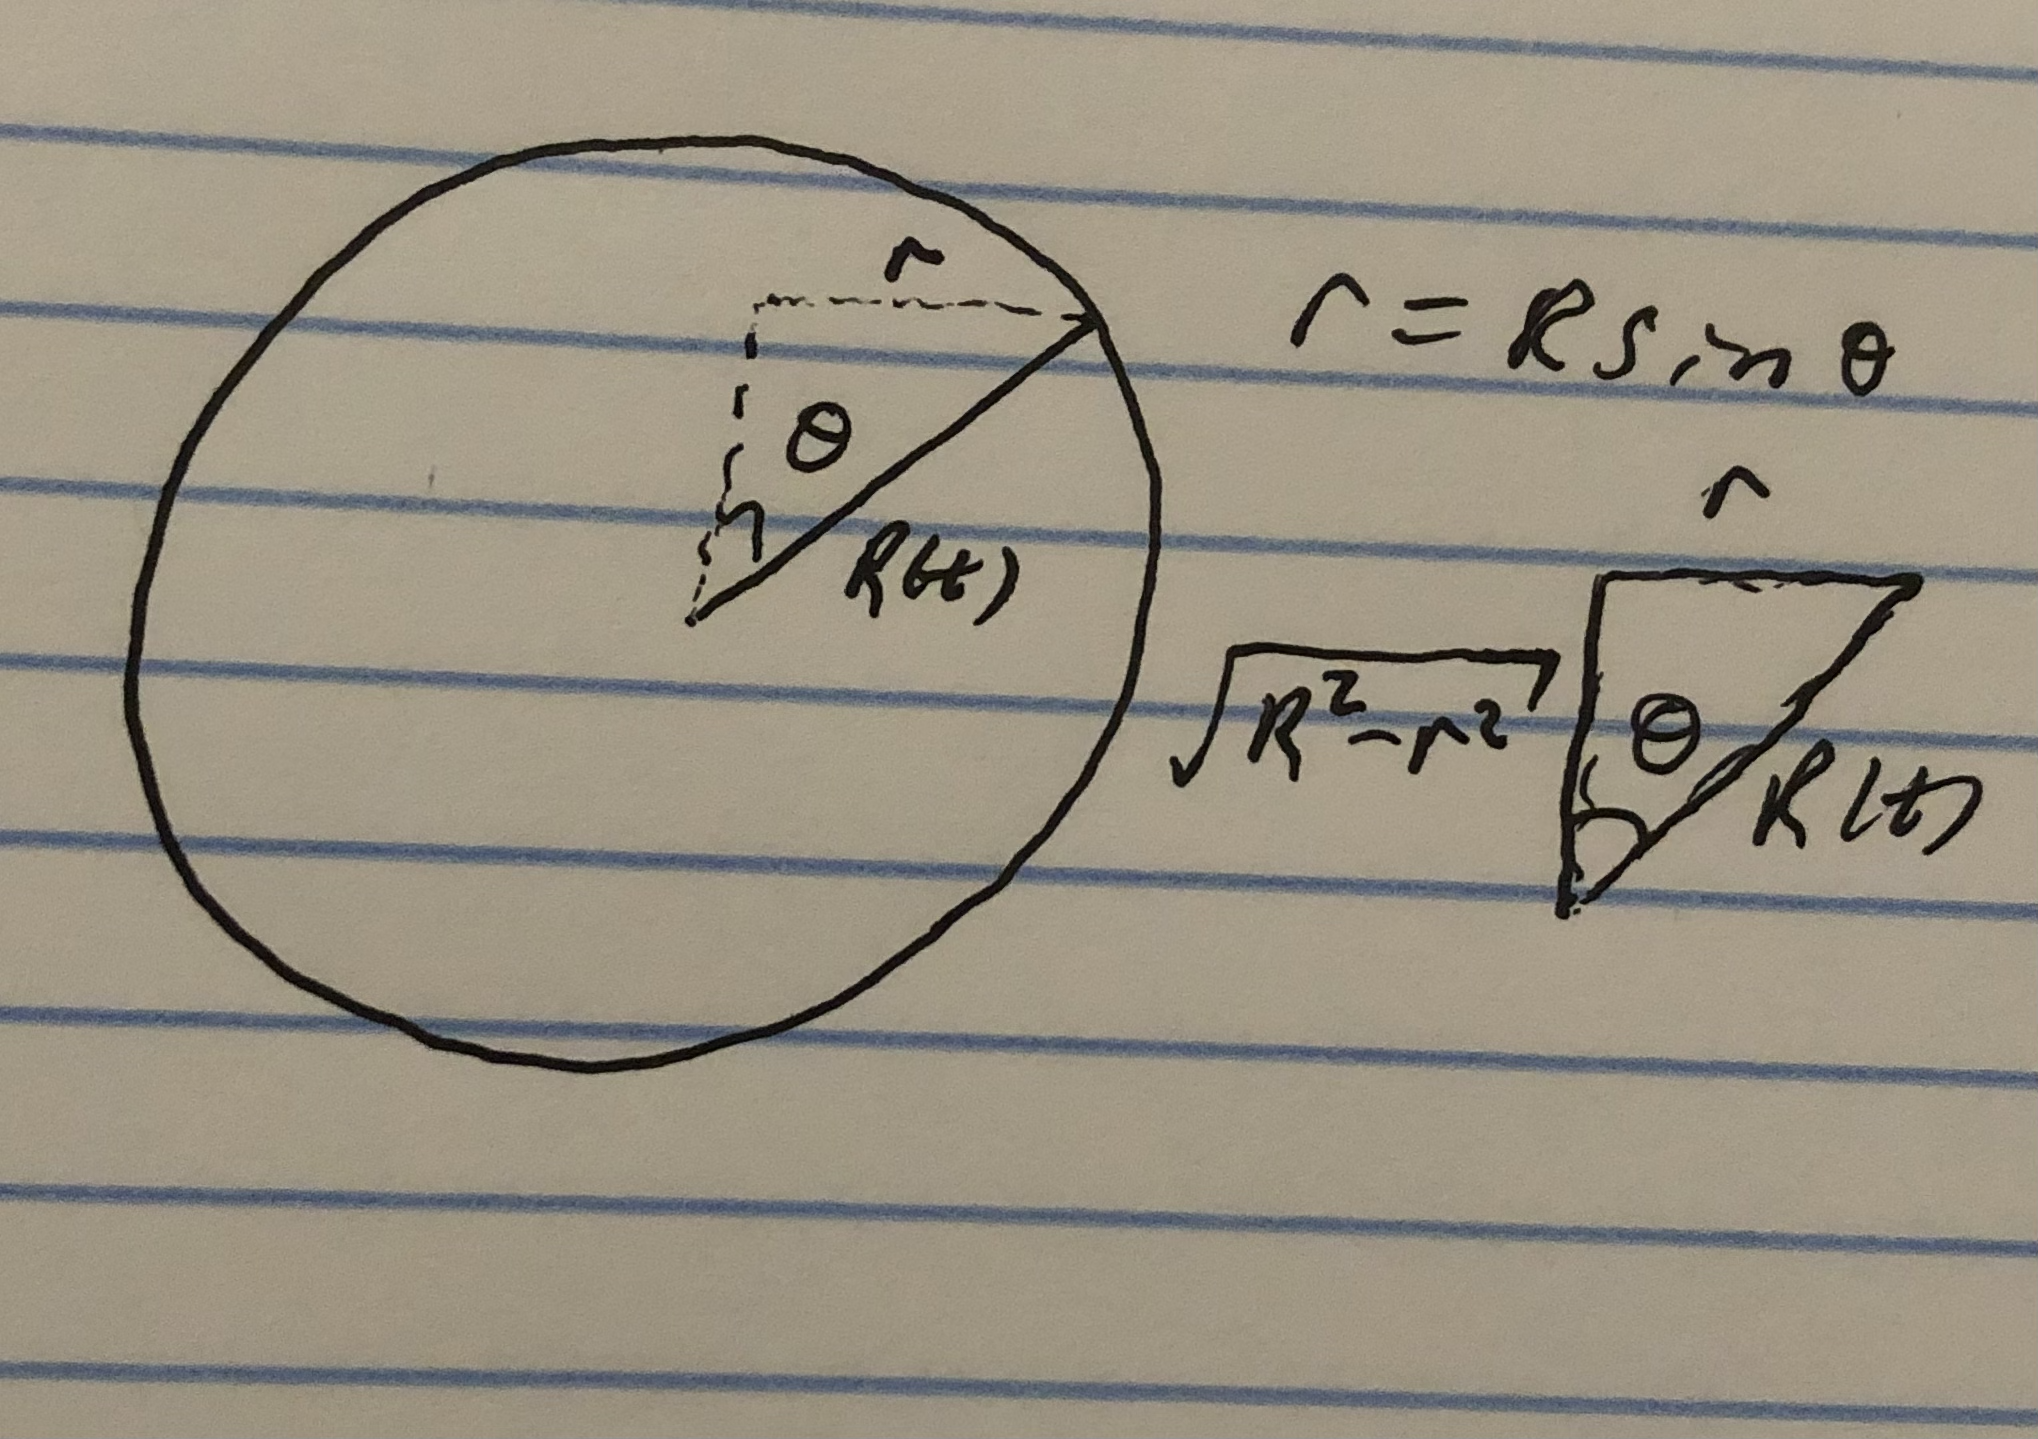
\includegraphics[scale=.15]{Figures/FRW_im.png}
    \caption{FRW 2D sphere}
    \label{fig:fig2}
\end{figure}
We start with a sphere of radius R, the line element on the surface of the sphere is given by
$$(d \ell)^2 = ( R d \theta)^2 + (r d \phi)^2$$
where,
$$r= R \sin \theta \implies dr = R \cos \theta d \theta.$$
$$\implies R d \theta = \frac{dr}{\cos \theta} = \frac{dr}{\sqrt{1- \frac{r^2}{R^2}}} = \frac{dr}{\sqrt{1- K r^2}}\\
\implies ( d \ell)^2 = ( \frac{dr}{\sqrt{ 1- K r^2}})^2 + (r d \phi)^2\\$$
more generally $K = \frac{k}{R^2}.$ To solve for $\sin \theta$ we note
$$r(t_0) = R(t_0) \sin \theta$$
$$\implies \frac{r(t_0)}{R(t_0)} = \sin \theta$$
$$\implies r(t) = R(t) \frac{r(t_0)}{R(t_0)} = R(t) x,$$
where we have defined $x= \frac{r(t_0)}{R(t_0)}.$ Plug in $dr$ and $r$ in terms of $R$ and $x$ to obtain,
$$\implies (d \ell)^2 = R^2(t) \left [ \frac{dx^2}{\sqrt{1 - k x^2}} + ( x d \phi)^2 \right].$$
There is no reason in an isotropic, homogeneous universe why time should pass differently at each point in space and we know locally it should pass the same in flat space, so\\
$$ds^2 = (c dt)^2 - R^2(t) \left[ \frac{dx^2}{1-k x^2} + ( x d \phi)^2 \right]$$\\
relabel
$x \rightarrow r$ and obtain\\
$$ ds^2 = (c dt)^2 - R^2(t) \left[ \frac{dr^2}{1- kr^2} + (r d \phi)^2 \right].\\$$
This is the FRW metric for a 3D spacetime, to generalize this to 4 dimensions we make the heuristic replacement,
$$d \phi^2 \rightarrow d\Omega^2= (d \theta)^2 + (\sin \theta d \phi)^2.$$
Therefore,\\
$$ds^2= (c dt)^2 - ( \frac{dr}{\sqrt{1-k r^2}})^2 - (r d \theta)^2 - (r \sin \theta d \phi)^2$$


\item 
\subsection{Derivation of $p_v = - \rho_v$}
Recall some basic facts from General Relativity,
$$G_{\mu \nu} - \Lambda g_{\mu \nu} = 8 \pi G T_{\mu \nu},$$ 
where $G_{\mu \nu}$ is the Einstein tensor given by,
$$G_{\mu \nu} = R_{\mu \nu} - \frac{1}{2} R g_{\mu \nu},$$ 
and for a perfect fluid we have,
$$T_{\mu \nu} = ( p_s + \rho_s) U_{\mu} U_{\nu} - p_s g_{\mu \nu}.$$
Or in flat space, for a perfect fluid we would expect it to not be viscous meaning no sliding friction, which implies all off diagonal quantities would be zero, so the flux of the time momentum (energy) through the time surface would be $\rho$ and the flux of the $i$ momentum through the $i$ surface would just be the momentum flux or the pressure. So,
$$T_{\mu \nu} = \begin{pmatrix} \rho & 0 & 0 & 0 \\ 0 & p & 0 & 0 \\ 0 & 0 & p & 0 \\ 0 & 0 & 0 & p \end{pmatrix}$$.
Written another way we have,
$$T_{\mu \nu} = ( p_s + \rho_s) U_{\mu} U_{\nu} - p_s \eta_{\mu \nu},$$
so in curved space, the generalization would obviously be given by $T_{\mu \nu}$ with the substitution $\eta_{\mu \nu} \rightarrow g_{\mu \nu}$
and in the rest frame of the fluid $U$ is given by $U^{\mu} \rightarrow (1,0,0,0).$ The
 $(-)$ sign on $\Lambda g_{\mu \nu}$ and $p_s g_{\mu \nu}$ terms are because our metric has a -2 signature, it would be flipped otherwise. Rearranging the EFE's we obtain,\\
$$ G_{\mu \nu} = 8 \pi G ( T_{\mu \nu} + \frac{\Lambda}{8 \pi G} g_{\mu \nu}) = 8 \pi G T'_{\mu \nu}$$
where $T'_{\mu \nu} = T_{\mu \nu} + \frac{\Lambda}{8 \pi G} g_{\mu \nu}$ is the modified stress-energy tensor.\\
To obtain the modified energy density, we compute the 00 component of T
$$T_{00}' = T_{00} + \frac{\Lambda}{8 \pi G} g_{00} = \rho_s + \frac{\Lambda}{8 \pi G} = \rho_s + \rho_v\\$$
where $\rho_v = \frac{\Lambda}{8 \pi G}.$\\
To compute the modified pressure we compute $T_{rr}'$.
$$T_{rr}' = T_{rr} + \frac{\Lambda}{8 \pi G} g_{rr}$$
$$= ( p_s + \rho_s) U_r U_r - p_s g_{rr} + \frac{\Lambda}{8 \pi G} g_{rr}$$
$$= - p_s g_{rr} + \frac{\Lambda}{8 \pi G} g_{rr} = (- g_{rr})(p_s - \frac{\Lambda}{8 \pi G})$$\\
$$\implies p= p_s - \frac{\Lambda}{8 \pi G} = p_s - \rho_v\\$$
therefore,\\
$$p_v = - \rho_v$$\\
$-g_{rr}>0$ due to our choice of signature, it is much more intuitive for a +2 signature.
In the rest of the paper we relabel $T'_{\mu \nu} \rightarrow T_{\mu \nu}$



\item \underline{$\rho_j(a) = C a^{-3(1+ w_j)} \propto \begin{cases} a^{-3} \rm{\,\,non-rel} \\ a^{-4} \rm{\,\,relativistic \,\,rad} \\ \rm{const} \rm{\,\,vacuum} \end{cases}$}\\
\underline{recall:} $\frac{d}{dt} ( \rho_j a^3) = - p_j \frac{d}{dt} a^3\\
\implies \dot{\rho}_j a^3 + \rho_j 3 a^2 \dot{a} =- p_j 3 a^2 \dot{a}\\$
\underline{recall:} $p_j(t) = w_j \rho_j,\,\, w_j = \begin{cases} 0\,\, \rm{ \,\,nonrelativistic\,\,matter} \\ 1/3 \,\,\rm{ \,\,relativistic\,\,radiation}\\
-1 \rm{   \,\,vacuum} \end{cases}\\
\implies \dot{\rho}_j + 3 \rho_j (1 + w_j) \frac{\dot{a}}{a} = 0\\
\implies \log \rho_j = - 3 ( 1 + w_j) \log a + C\\
\implies \rho_j(a) = C a^{-3(1+ w_j)}$\\


\hdashrule[0.5ex][c]{\linewidth}{0.5pt}{1.5mm}

\item \underline{$\frac{\ddot{a}}{a} = - \frac{1}{2} \frac{\rho_t}{3 M_{pl}^2} - \frac{p}{2 M_{pl}^2} = - \frac{\rho_t(t) + p(t)}{6 M_{pl}^2}$}\\
\underline{recall:} $\frac{2 \ddot{a}}{a} + ( \frac{\dot{a}}{a})^2 + \frac{k}{a^2} = - \frac{p}{M_{pl}^2}$\\ (11 component of einsteins field equations)\\
$\implies \frac{\ddot{a}}{a} = - \frac{1}{2} (( \frac{\dot{a}}{a})^2 + \frac{k}{a^2}) - \frac{p}{2 M_{pl}^2}\\$
\underline{recall:} $\frac{\dot{a}^2}{a^2} + \frac{k}{a^2} = \frac{\rho_t}{3 M_{pl}^2}$ (00 component of einsteins field equations)\\
$\implies \frac{\ddot{a}}{a} = - \frac{1}{2} \frac{\rho_t}{3 M_{pl}^2} - \frac{p}{2 M_{pl}^2} = - \frac{\rho_t(t) + p(t)}{6 M_{pl}^2}\\$


\hdashrule[0.5ex][c]{\linewidth}{0.5pt}{1.5mm}


take $p_j = w_j \rho_j$ derivation from notes\\


\hdashrule[0.5ex][c]{\linewidth}{0.5pt}{1.5mm}


\item \underline{$a(t) \propto t^{\beta};\,\, \beta = \frac{2}{3 + 3 w_j}$}\\
\underline{recall:} $\frac{\ddot{a}}{a} = - \frac{1 + 3 w_j}{6 M_{pl}^2} \rho_j,\,\, \rho_j = C a^{-3(1+w_j)}\\
\implies \frac{\ddot{a}}{a} = - \frac{1 + 3 w_i}{6 M_{pl}^2} C a^{-3(1+ w_j)}\\
\implies \ddot{a} a^{2 + 3 w_j} =$ const;\,\, assume $a \propto t^{\beta}\\
\implies \beta(\beta - 1) t^{\beta-2} t^{2 \beta + 3 \beta w_j} = \rm{const}\\
\implies t^{3 \beta + 3 \beta w_j -2} = \rm{const}\\
\implies 3 \beta + 3 \beta w_j -2 =0 \implies \beta = \frac{2}{3(1+w_j)}$


\hdashrule[0.5ex][c]{\linewidth}{0.5pt}{1.5mm}


\item \underline{$a(t) \sim \begin{cases} t^{2/(3+3w_j)} \\ e^{\sqrt{\Lambda(t)/3} t} \rm{\,\,vacuum} \end{cases} = \begin{cases} t^{2/3} \rm{\,\,non-relativistic\,\,matter} \\ t^{1/2} \rm{\,\,relativistic\,\,radiation} \end{cases}$}\\
\underline{recall:} $a(t) = t^{\beta},\,\, \beta = \frac{2}{3 + 3 w_j}\\
\implies H(t) = \frac{\dot{a}}{a} = \frac{\beta t^{\beta - 1}}{t^{\beta}} = \frac{2}{3 + 3 w_j} \frac{1}{t}\\$
does not work for $w_{vac} = -1\\$
\underline{recall:} 1.17\\
\underline{recall:} $\frac{\dot{a}^2}{a^2} + \frac{k}{a^2} = \frac{\rho_t}{3 M_{pl}^2} = \frac{\rho_m + \rho_r + \rho_{\Lambda}}{3 M_{pl}^2}\\$
vacuum energy $\implies \rho_r = \rho_m = k = 0\\
\implies \frac{\dot{a}^2}{a^2} = \frac{\rho_{\Lambda}}{3 M_{pl}^2}\\$
\underline{recall:} $\frac{\Lambda(t)}{3 H(t)^2} = \frac{\rho_{\Lambda}(t)}{\rho_c(t)} \implies \rho_{\Lambda}(t) = \frac{\Lambda \rho_c}{3 H^2} = \frac{3 H^2 M_{pl}^2 \Lambda}{3 H^2}\\
= \Lambda M_{pl}^2\\
\implies \frac{\dot{a}^2}{a^2} = \frac{\Lambda(t)}{3},\,\,$ recall $\rho_{vac} = \rm{const.} = \rho_{\Lambda} \implies \Lambda(t) = \Lambda\\
\implies \frac{\dot{a}}{a} = \sqrt{\frac{\Lambda}{3}} = H \implies a(t) \propto e^{\pm \sqrt{\Lambda(t)/3} t}$ choose positive since universe expands


\hdashrule[0.5ex][c]{\linewidth}{0.5pt}{1.5mm}


$a(T) \propto \frac{1}{T}$ (results from stefan boltzmann law, set equal to radiation dominated universe)\\


\hdashrule[0.5ex][c]{\linewidth}{0.5pt}{1.5mm}


\item \underline{$H(t)^2 = ( \frac{1}{2t})^2 = \frac{\rho_r}{3 M_{pl}^2} = \frac{1}{3 M_{pl}^2} \frac{\pi^2}{30} g_{eff}(T) T^4\\
=( \frac{ \phi \sqrt{g_{eff}}}{\sqrt{90}} \frac{T^2}{M_{pl}^2})^2$}\\
 (relativistic-radiation dominated universe)\\


\underline{recall:} $H(t) = \frac{1}{2t}\\$
\underline{recall:} $H(t)^2 = \frac{\rho_m(t) + \rho_r(t)}{3 M_{pl}^2} = \frac{\rho_r}{3 M_{pl}^2}\\$
\underline{recall:} $\rho_r(t) = \rho_{bosons}(t) = \frac{\pi^2}{30} g_{eff}(T) T^4\\
\implies H(t)^2 = \frac{1}{3 M_{pl}^2} \frac{\pi^2}{30} g_{eff}(T) T^4$


\hdashrule[0.5ex][c]{\linewidth}{0.5pt}{1.5mm}


\section*{Dark Matter}
\item \underline{$\frac{d Y(t)}{dt} = - \langle \sigma_{\chi \chi} v \rangle T(t)^3 (Y(t)^2 - Y_{eq}(t)^2)$} $Y(t) := \frac{n(t)}{T^3}\\$
\underline{recall:} $\dot{n} + 3 H(t) n(t) = \frac{1}{a(t)^3} \frac{d}{dt} (n(t) a(t)^3) = - \langle \sigma_{\chi \chi} v \rangle (n(t)^2 - n_{eq}(t)^2)\\
\implies T(t)^3 \frac{d}{dt} ( \frac{n(t)}{T(t)^3}) = - \langle \sigma_{\chi \chi} v \rangle (n(t)^2 - n_{eq}(t)^2)\\
\implies \frac{d}{dt} Y(t) = - \langle \sigma_{\chi \chi} v \rangle T(t)^3 ( \frac{n(t)^2}{T(t)^6} - \frac{n_{eq}(t)^2}{T(t)^6})\\
= - \langle \sigma_{\chi \chi} v \rangle T(t)^3 (Y(t)^3 - Y_{eq} (t)^3)\\$


\hdashrule[0.5ex][c]{\linewidth}{0.5pt}{1.5mm}


\hdashrule[0.5ex][c]{\linewidth}{0.5pt}{1.5mm}


\item \underline{$\Omega_{\chi} h^2 = 0.12 \frac{x_{dec}}{23} \frac{\sqrt{g_{eff}}}{10} \frac{1.7 E -9 GeV^{-2}}{\langle \sigma_{\chi \chi} v \rangle}$}\\
assume DM decoupling happens when $\rho_r >> \rho_m$\\
i.e. radiation dom (early universe)\\
Let $x = \frac{m_{\chi}}{T} and x = 1 \implies m_{\chi} = T\\$
\underline{Note:} $H(x=1) = \frac{\pi \sqrt{g_{eff}}}{\sqrt{90}} \frac{T^2}{M_{pl}} = \frac{\pi \sqrt{g_{eff}}}{\sqrt{90}} \frac{m_{chi}^2}{M_{p.}} \frac{T^2}{T^2} = \frac{\pi sqrt{g_{eff}}}{\sqrt{90}} \frac{T^2}{M_{pl}} ( \frac{m_{\chi}}{T})^2\\
= H(t) x^2 \implies H(t) = \frac{H(x=1)}{x^2}\\
\implies \frac{1}{2t} = H = \frac{H(x=1)}{x^2} \implies x = \sqrt{2t H(x=1)}\\
\implies \frac{dx}{dt} = \frac{d(2t)}{dt} H(x=1) \frac{1}{2} \frac{1}{\sqrt{2t H(x=1)}} = \frac{H(x=1)}{\sqrt{2t H(x=1)}} \\
= \frac{H(x=1)}{x}$


\hdashrule[0.5ex][c]{\linewidth}{0.5pt}{1.5mm}



\section*{Cosmology}


\item \underline{$g^*(T) = \sum_{bos} g_i( \frac{T_i}{T})^4 + \frac{7}{8} \sum_{fer} g_i ( \frac{T_i}{T})^4$}\\
\underline{recall:} $\rho(T) = \begin{cases} \frac{7}{8} \frac{\pi^2}{30} g T^4 (\text{fermions})\\
\frac{\pi^2}{30} g T^4 (\text{bosons}) \end{cases}\\
\rho = \sum_i \rho_i = \sum_i \frac{\pi^2}{30} g_i T_i^4 + \frac{7}{8} \sum_i \frac{\pi^2}{30} g_i T_i^4\\
= \frac{\pi^2}{30} ( \sum_b g_v T_b^4 + \frac{7}{8} \sum_f g_f T_f^4) \frac{T^4}{T^4}\\
= \frac{\pi^2}{30} ( \sum_b g_b \frac{T_b^4}{T^4} + \frac{7}{8} \sum_f g_f \frac{T_f^4}{T^4})T^4\\
= \frac{\pi^2}{30} g^*(T) T^4\\
\therefore g^*(T) = \sum_b g_b ( \frac{T_b}{T})^4 + \frac{7}{8} \sum_f g_f ( \frac{T_f}{T})^4$


\hdashrule[0.5ex][c]{\linewidth}{0.5pt}{1.5mm}


In the very early universe, massive particles can be neglected since they are non relativistic and only the relativistic particles need to be considered. Before this all particles were unified, and hence all 3 forces were unified, before this it is thought that gravity was also unified. However at some point electroweak and QCD sectors became distinct forces, after this electroweak sector decouples and it is at this point that all particles can be considered. However back to where we first started the universe was highly relativistic so the main interactions come from the relativistic particles such as photons and neutrinos. It seems like there is a temperature where each species of particles become non relativistic and this is when they annihilate with each-other, each time leaving a relic density that freezes out due to an initial asymmetry in each sector. It seems like the largest particles annihilate first and freeze out then smaller? 

The number densities that we are used too (all of them?) are only for free particles. Neutrinos freeze out when the expansion rate is bigger than the interaction rate, which is when they fall out of thermal equilibrium, (do antineutrinos exist? Neutrinos have no charge so they do not have antiparticles, same with photons). it seems like all the other particles annihilate at which their density freezes out once all antiparticles have annihilated.

Need to understand $T<100$ MeV better, especially how pions disappear. Also the last calculation of the effective degrees of freedom I do not understand at all.

the following is a very illustrative exercise to know how the universe and the particle densities fell out of equilibrium, a species of particle $i$ annihilates when $T_i<m_i$\\

$g_*(T) = \sum_{bos} g_i ( \frac{T_i}{T})^4 + \frac{7}{8} \sum_{fer} g_i ( \frac{T_i}{T})^4\\$
$g_b = 8 \times 2$ (gluons)$+$phot 2$+ W^{\pm}  Z^0 3 \times 3,+ $Higgs 1 = 28\\
\underline{Note:} gluons have 3 spin states but they are massless so gauge freedom kills off one of the spins, W bosons are massive so they keep 3 spin states
$g_f = 90$ quarks $12 \times 6,\,\,$ charged leptons 6$ \times$ 2, neutrinos 3 $\times$ 2\\
early universe $\implies T_i = T \forall i$, ( thermal equilibrium)\\
$g_*(T) = 28 + \frac{7}{8} \cdot 90 = 106.75\\$
recall thermal equilibrium basically tells us when $\gamma$ creates $e^- e^+$ then the reverse reaction happens at the same rate\\
top quark becomes non-relativistic, annihilates then freezes out
\item \underline{$T \sim 200$ GeV} all particles are relativistic and present, in thermal equilibrium $g_{*} (T)$\\
\item \underline{$T< 170$ Gev} top quark annihilates\\
$g_{*}(T) = \sum_{bos} g_i ( \frac{T_i}{T})^4 + \frac{7}{8} \sum_{fer} g_i ( \frac{T_i}{T})^4\\
g_{*}(T) = 28 + 68.25 = 96.25$ ( just insert 5 instead of 6 for quark, top quark is not included and this replacement accounts for antiparticle)\\
\item \underline{$T \sim 160$ GeV} EW crossover (no effect)\\
\item \underline{$T < 125$ GeV} $H^0$ annihilates\\
$g_{H^0} =1 \implies g_*(T) = 96.25 - 1 = 95.25\\$
\item \underline{$T< 80$ GeV} $W^{\pm},\,\,Z^0\\$
$g_{W^{\pm}} = 3+3 = 6, W^-$ is antiparticle of $W^+ g_{Z^0} = 3\\$
$\implies g_{W^{\pm} Z^0 } = 9 \implies g_*(T) = 95.25-9 = 86.25\\$
\item \underline{$T< 4 GeV$} bottom annihilates\\
$g_*(T) = 8 \times 2 + 2 + \frac{7}{8} ( 12 \times 4 + 6\times2 + 3\times2)= 75.75\\$
\item \underline{$T< 1$ GeV} charm quark, $\tau^-$ annihilates\\
$g_{eff}(T) = 8\times2 + 2 + \frac{7}{8} ( 12 \times 3 + 2 \times2\times2 + 3 \times 2 ) = 61.75\\$
\item \underline{$T \sim 100$ MeV} QCD crossover ( $u,d, s~\rm{strange},g\sim \rm{gluon} \rightarrow \pi^{\pm, 0}$)\\
$g_*(T) = 2 + \frac{7}{8} (5 \times 2 + 2 \times 2) + 3$ ( for pions) = 17.25\\
all quarks become 2 quark systems (mesons) or 3 quark systems (baryons)\\
(do each of meson/baryons contain all 8 gluons?)\\
each pion has spin 0 and a charge associated $\pi^0 \sim$ charge\\
$\pi^{+}, \pi^-$ are antiparticles of each-other hence $g={\pi^{\pm,0}} = 3$\\
\item \underline{$T< 100$ MeV}$ \pi^{\pm},\,\, \pi^0,\,\, \mu^-\\$
$(\pi^{\pm}$ annihilate? $\pi^0$ annihilates with itself? $\mu^-$ annihilates $\nu_{\mu}$ leaves relic) $e^{\pm} \nu \bar{\nu} \gamma$ left ($\nu$ includes all 3 species of particles)\\
$\implies g_*(T) = 2 + \frac{7}{8} (1 \cdot 2 \cdot 2 + 3 \cdot 2)= 10.75\\$
\item \underline{$T< 500$ KeV} $e^-$ annihilates with $e^+$ (neutrinos have stayed in equilibrium the whole time (what kind of equilibrium?))\\
$g_*(T) = 2 + 5.25 (4/11)^{4/3}\\$


\hdashrule[0.5ex][c]{\linewidth}{0.5pt}{1.5mm}


up until now particles are kept into thermal equillibrium by thermal interactions. However once positrons/electrons annihilate. (neutrinos interact via the weak forc) they are no longer in thermal equillibrium\\
(unless $T \propto a^{-1}$ but annihilation deviate this, dont understand?) elecgtron positron annihilations produce $\gamma$ which heats photon background\\
\underline{Note:} $T_{\nu} \propto a^{-1}\\$


\hdashrule[0.5ex][c]{\linewidth}{0.5pt}{1.5mm}


\item \underline{$g_* (T) = 2 + 5.25 ( \frac{4}{11})^{4/3} = 3.363$} (neutrino photon bath)\\
The reason we still include the neutrinos even after they decouple is because unlike the other particles, neutrinos still remain relativistic, but note we do not know the mass of neutrinos we just know they are less than some mass, hence how the mass appears on a particle physics table.
\underline{recall:} $g_{*s}(T) T^3 a(t)^3 = const;\,\, g_{*s}(T) = \sum_{bos} g_i ( \frac{T_i}{T})^3 + \frac{7}{8} \sum_{fermions} g_i ( \frac{T_i}{T})^3\\
\implies g_{*s} T^3 a(t)^3 = (2 T_{\gamma}^3 + \frac{7}{8} 6 T_{\nu}^3) a(t)^3\\
1 \sim before e^+, e^- annihilation;\,\, 2 \sim After e^+, e^- annihilation\\
g_{*s}(T_1) T_1^3 a_1^3 = g_*(T_1) T_1^3 a_1^3 = 10.75 T_1^3 a_1^3\\
g_{*s} (T_2) T_2^3 a_2^3 = (2 T_2^3 a_2^3 + 5.25 T_{\nu_2}^3 a_2^3\\$
(Why do we take $T= T_{\gamma}$?)\\
$a_1^3 T_1^3 = a_1^3 T_{\nu_1}^3 = a_2^3 T_{\nu_2}^3\\
\implies 10.75 T_1^3 a_1^3 = 2 T_2^3 a_2^3 + 5.25 T_1^3 a_1^3\\
\implies 10.75 a_2^3 T_{\nu_2}^3 = 2 T_2^3 a_2^3 + 5.25 a_2^3 T_{\nu_2}^3\\$
Let $T_{\nu_2} \rightarrow T_{\nu},\,\, T_2 \rightarrow T\\
\implies 10.75 = 2 ( \frac{T}{T_{\nu}})^3 + 5.25\\
\implies \frac{T_{\nu}}{T} = ( \frac{4}{11})^{1/3}\\
\therefore g_*(T) = 2 + 5.25 (\frac{T_{\nu}}{T})^4 = 2 + 5.25 ( \frac{4}{11})^{4/3} = 3.636\\$


\hdashrule[0.5ex][c]{\linewidth}{0.5pt}{1.5mm}


neutrino background is non-relativistic today\\
a particle will annihilate when $T< m_i$\\
(this might give us intuition on how they stay in thermal equilibrium before annihilation\\
Baryon number resides in nucleons (Protons and neutrons)\\
(they are lightest baryon)\\
$n_B = n_N - N_{\bar{N}}= n_p + n_n - n_{\bar{p}} - n_{\bar{n}}\\\\
\eta= \frac{n_B(t_0)}{n_{\gamma} (t_0)} \approx 6 E -10$ (since this is after annihilation did $\eta=1$ before annihilation?)\\
after annihilation baryon number is conserved\\
$\implies N_B = n_B V \propto n_B a^3(t) = const\\ \implies n_B \propto a^{-3}(t)\\
\implies n_B (T) = \eta n_{\gamma}(T) = \eta \frac{2 \zeta (3)}{\pi^2} T^3,\,\, T< m_e\\$
tot number of protons = tot number of electrons\\
$n_p^* = n_e^* = n_{e^-} \sim free\\
\implies n_N^* = n_n^* + n_p^* = n_B\\$
need to understand nucleosynthesis\\
i.e. how protons and neutrons came to be\\
then comes recombination $\sim 10 \%$ He atoms and rest is $n_{e^-} = n_p^*$ and $n_H \sim$ neutral hydrogen \\
before this $e^-, p , \gamma,$ (n?) were in thermal equilibrium\\
after recombination universe becomes transparent and $n_H$ forms (don't understand this, I though they fell out of thermal equilibrium a long time ago?)


\hdashrule[0.5ex][c]{\linewidth}{0.5pt}{1.5mm}


when $T$ became low enough $e^-, p, n$ form neutral atoms $e^-$ fell sharply,\\
$e^-$ no longer can communicate with $\gamma$, fall out of thermal equillibrium\\
$e^- + p \rightarrow H + \gamma \implies \gamma$ heats up, since $\gamma$ is increasing from the forward reaction\\


\hdashrule[0.5ex][c]{\linewidth}{0.5pt}{1.5mm}


$n_B = n_p + n_H,\,\, n_p \sim$ free\\


\hdashrule[0.5ex][c]{\linewidth}{0.5pt}{1.5mm}


\item \underline{$n_i = g_i (\frac{m_i T}{2 \pi})^{3/2} \exp[ \frac{\mu_i - m_i}{T}]$}\\
\underline{recall:} $n = g ( \frac{m T}{2 \pi})^{3/2} e^{- (m-\mu)/T}$ (nonrelativistic)\\


\hdashrule[0.5ex][c]{\linewidth}{0.5pt}{1.5mm}


$p + e^- \leftrightarrow H + \gamma,\,\,$ (chem eq.) $\implies \mu_p + \mu_e = \mu_H\\$


\hdashrule[0.5ex][c]{\linewidth}{0.5pt}{1.5mm}


\item \underline{$n_H = \frac{g_H}{g_p g_e} n_p n_e ( \frac{m_e T}{2 \pi})^{-3/2} e^{B/T}$}
$; B= m_p + m_e - m_H = 13.6\\
n_H = g_H ( \frac{m_H T}{2 \pi})^{3/2} e^{\frac{\mu_H - m_H}{T}}\\
= g_H ( \frac{(m_p + m_e - B)T}{2 \pi} )^{3/2} e^{\frac{\mu_p - m_p}{T}} e^{\frac{\mu_e - m_e}{T}} e^{B/T}\\
= \frac{g_H}{g_p g_e} ( \frac{m_e T}{2 \pi})^{-3/2} ( \frac{m_p T}{2 \pi})^{-3/2} ( \frac{(m_p + m_e - B)T}{2 \pi})^{3/2} n_p n_e e^{B/T}\\
m_p \approx m_H \implies m_p + m_e - B = m_H \implies m_e = B\\
\therefore n_H = \frac{g_H}{g_p g_e} n_p n_e ( \frac{m_e T}{2 \pi})^{-3/2} e^{B/T}$


\hdashrule[0.5ex][c]{\linewidth}{0.5pt}{1.5mm}


\item \underline{$a \propto \frac{1}{T}$}\\
\underline{recall:} $\frac{\rho}{\rho_0} = ( \frac{a_0}{a})^4;\,\, d S = \frac{1}{T} dE + \frac{P}{T} d V\\
\implies S = \frac{E + P V}{T} = \frac{(\frac{E}{V} + P) V}{T} = \frac{( \rho + P) V}{T} \implies V = \frac{TS}P{\rho + P}\\$
assume expansion is adiabatic\\
\underline{recall:} $dQ = T ds,\,\, dQ = 0 \implies dS = 0 \implies S_0 = S\\
\implies \frac{V}{V_0} = \frac{\frac{TS}{\rho + P}}{\frac{T_0 S}{\rho_0 + P_0}} = \frac{TS}{\rho + P} \frac{\rho_0 + P_0}{T_0 S}\\$
\underline{recall:} $P = \frac{\rho}{3}\\$ (relativistic)
$\implies \frac{V}{V_0} = \frac{T}{T_0} \frac{\rho_0 + \frac{\rho_0}{3}}{\rho + \frac{\rho}{3}} = \frac{T}{T_0} \frac{\rho_0}{\rho} = \frac{T}{T_0} ( \frac{a}{a_0})^4 = ( \frac{a}{a_0})^3\\
\implies \frac{T}{T_0} \frac{a}{a_0} = 1 \implies a= \frac{a_0 T_0}{T}\\
\therefore a \propto \frac{1}{T}$


\hdashrule[0.5ex][c]{\linewidth}{0.5pt}{1.5mm}


\item \underline{$\frac{d}{dt} (\rho a^3) = - p \frac{d}{dt} (a^3)$}\\
start w/ FRW metric and use $G_{\alpha \beta} = 8 \pi T_{\alpha \beta}\\$
to calculate $T_{\alpha \beta}\\$
\underline{recall:} $T^{\alpha \beta}_{; \beta} = 0\\
\implies a^3 \dot{\rho} + 3 \rho a^2 \dot{a} + 3 p a^2 \dot{a}\\
= \frac{d}{dt} ( \rho a^3) + p \frac{d}{dt} a^3 = 0\\
\therefore \frac{d}{dt} ( \rho a^3) = - p \frac{d}{dt} ( a^3)\\$


\hdashrule[0.5ex][c]{\linewidth}{0.5pt}{1.5mm}


\item \underline{$\frac{d}{dt} ( \rho a^3) = 0$} (matter dominated)\\
main energy density is from matter assume non relativistic $\implies p = 0\\
\implies \frac{d}{dt} ( \rho a^3) = 0\\$


\hdashrule[0.5ex][c]{\linewidth}{0.5pt}{1.5mm}


\item \underline{$\frac{d}{dt} ( \rho a^4) = 0$} (rad dom)\\
\underline{recall:} $p = \frac{1}{3} \rho\\
\implies \frac{d}{dt} ( \rho a^3 ) = - p \frac{d}{dt} ( a^3) = - \frac{1}{3} \rho \frac{d}{dt} ( a^3)\\
\therefore \frac{d}{dt} (\rho a^4)$


\hdashrule[0.5ex][c]{\linewidth}{0.5pt}{1.5mm}


\item \underline{$\langle ( \frac{\Delta T}{T})^2 \rangle_{\theta} \approx \ell ( \ell+1) C_{\ell}/2 \pi$}\\
$\frac{\Delta T}{T} = \sum_{\ell, m} a_{\ell m} Y_{\ell m} ( \theta, \phi)\\$
no $\theta$ dependence means that all m terms for each l are identical\\
$C_{\ell} = \langle | a_{\ell m}|^2 \rangle = \frac{1}{2 \ell+1} \sum_{m=- \ell}^{\ell} | a_{\ell m}|^2\\
\langle ( \frac{\Delta T}{T})^2 \rangle_{\theta} \approx \ell( \ell+ 1) C_{\ell}/2 \pi\\$
this is what is plotted, the power spectrum plot is \\
$\langle ( \frac{\Delta T}{T})^2 \rangle_{\theta}$ v.s $\ell$


\end{enumerate}
\end{document}